\documentclass[a4paper]{book}
\usepackage{makeidx}
\usepackage{natbib}
\usepackage{graphicx}
\usepackage{multicol}
\usepackage{float}
\usepackage{listings}
\usepackage{color}
\usepackage{ifthen}
\usepackage[table]{xcolor}
\usepackage{textcomp}
\usepackage{alltt}
\usepackage{ifpdf}
\ifpdf
\usepackage[pdftex,
            pagebackref=true,
            colorlinks=true,
            linkcolor=blue,
            unicode
           ]{hyperref}
\else
\usepackage[ps2pdf,
            pagebackref=true,
            colorlinks=true,
            linkcolor=blue,
            unicode
           ]{hyperref}
\usepackage{pspicture}
\fi
\usepackage[utf8]{inputenc}
\usepackage{mathptmx}
\usepackage[scaled=.90]{helvet}
\usepackage{courier}
\usepackage{sectsty}
\usepackage[titles]{tocloft}
\usepackage{doxygen}
\lstset{language=C++,inputencoding=utf8,basicstyle=\footnotesize,breaklines=true,breakatwhitespace=true,tabsize=8,numbers=left }
\makeindex
\setcounter{tocdepth}{3}
\renewcommand{\footrulewidth}{0.4pt}
\renewcommand{\familydefault}{\sfdefault}
\hfuzz=15pt
\setlength{\emergencystretch}{15pt}
\hbadness=750
\tolerance=750
\begin{document}
\hypersetup{pageanchor=false,citecolor=blue}
\begin{titlepage}
\vspace*{7cm}
\begin{center}
{\Large \-Q\-M\-A\-S\-T \-Source \-Code }\\
\vspace*{1cm}
{\large \-Generated by Doxygen 1.7.5.1}\\
\vspace*{0.5cm}
{\small Fri Sep 30 2011 21:11:01}\\
\end{center}
\end{titlepage}
\clearemptydoublepage
\pagenumbering{roman}
\tableofcontents
\clearemptydoublepage
\pagenumbering{arabic}
\hypersetup{pageanchor=true,citecolor=blue}
\chapter{\-The \-Q\-M\-A\-S\-T \-Alpha 6 \-Sailing \-Code}
\label{index}\hypertarget{index}{}\begin{DoxyParagraph}{\-This \-Documentation}
\-Is the same style as the \-Java\-Doc documentation. \-The same commands are used in the code, and generates these pages. \-For info on the program used check out a program called \-Doxygen
\end{DoxyParagraph}
\begin{DoxyParagraph}{\-Revised by \-Laszlo 2011-\/05-\/13}
\-Ported to \-Arudino \-November 2010 by \-Christine and the supercool software team \-Created on\-: 2010-\/05-\/11 \-Author\-: \-Nader for \-M\-A\-S\-T \-Software 
\end{DoxyParagraph}

\chapter{\-Module \-Index}
\section{\-Modules}
\-Here is a list of all modules\-:\begin{DoxyCompactList}
\item \contentsline{section}{\-Globalconstants}{\pageref{group__globalconstants}}{}
\item \contentsline{section}{\-Serial\-Data}{\pageref{group__group1}}{}
\end{DoxyCompactList}

\chapter{\-Data \-Structure \-Index}
\section{\-Data \-Structures}
\-Here are the data structures with brief descriptions\-:\begin{DoxyCompactList}
\item\contentsline{section}{\hyperlink{structpoints}{points} }{\pageref{structpoints}}{}
\end{DoxyCompactList}

\chapter{\-File \-Index}
\section{\-File \-List}
\-Here is a list of all files with brief descriptions\-:\begin{DoxyCompactList}
\item\contentsline{section}{/\-Users/allgood38/\-Desktop/qmast/sailcode\-\_\-alpha6/\hyperlink{_data_acquisition_8pde}{\-Data\-Acquisition.\-pde} }{\pageref{_data_acquisition_8pde}}{}
\item\contentsline{section}{/\-Users/allgood38/\-Desktop/qmast/sailcode\-\_\-alpha6/\hyperlink{_location_struct_8h}{\-Location\-Struct.\-h} }{\pageref{_location_struct_8h}}{}
\item\contentsline{section}{/\-Users/allgood38/\-Desktop/qmast/sailcode\-\_\-alpha6/\hyperlink{_menu_8pde}{\-Menu.\-pde} }{\pageref{_menu_8pde}}{}
\item\contentsline{section}{/\-Users/allgood38/\-Desktop/qmast/sailcode\-\_\-alpha6/\hyperlink{_motor_control_functions_8pde}{\-Motor\-Control\-Functions.\-pde} }{\pageref{_motor_control_functions_8pde}}{}
\item\contentsline{section}{/\-Users/allgood38/\-Desktop/qmast/sailcode\-\_\-alpha6/\hyperlink{_navigation_code_8pde}{\-Navigation\-Code.\-pde} }{\pageref{_navigation_code_8pde}}{}
\item\contentsline{section}{/\-Users/allgood38/\-Desktop/qmast/sailcode\-\_\-alpha6/\hyperlink{oldtack_8pde}{oldtack.\-pde} }{\pageref{oldtack_8pde}}{}
\item\contentsline{section}{/\-Users/allgood38/\-Desktop/qmast/sailcode\-\_\-alpha6/\hyperlink{_parsing_functions_8pde}{\-Parsing\-Functions.\-pde} }{\pageref{_parsing_functions_8pde}}{}
\item\contentsline{section}{/\-Users/allgood38/\-Desktop/qmast/sailcode\-\_\-alpha6/\hyperlink{sailcode__alpha6_8pde}{sailcode\-\_\-alpha6.\-pde} }{\pageref{sailcode__alpha6_8pde}}{}
\item\contentsline{section}{/\-Users/allgood38/\-Desktop/qmast/sailcode\-\_\-alpha6/\hyperlink{_sailing_logic_8pde}{\-Sailing\-Logic.\-pde} }{\pageref{_sailing_logic_8pde}}{}
\item\contentsline{section}{/\-Users/allgood38/\-Desktop/qmast/sailcode\-\_\-alpha6/\hyperlink{_station_keeping_8pde}{\-Station\-Keeping.\-pde} }{\pageref{_station_keeping_8pde}}{}
\item\contentsline{section}{/\-Users/allgood38/\-Desktop/qmast/sailcode\-\_\-alpha6/\hyperlink{_tack_8pde}{\-Tack.\-pde} }{\pageref{_tack_8pde}}{}
\item\contentsline{section}{/\-Users/allgood38/\-Desktop/qmast/sailcode\-\_\-alpha6/\hyperlink{_testing___functions_8pde}{\-Testing\-\_\-\-Functions.\-pde} }{\pageref{_testing___functions_8pde}}{}
\item\contentsline{section}{/\-Users/allgood38/\-Desktop/qmast/sailcode\-\_\-alpha6/\hyperlink{_transmit_8pde}{\-Transmit.\-pde} }{\pageref{_transmit_8pde}}{}
\item\contentsline{section}{/\-Users/allgood38/\-Desktop/qmast/sailcode\-\_\-alpha6/\hyperlink{_utilities_8pde}{\-Utilities.\-pde} }{\pageref{_utilities_8pde}}{}
\end{DoxyCompactList}

\chapter{\-Module \-Documentation}
\hypertarget{group__globalconstants}{
\section{\-Globalconstants}
\label{group__globalconstants}\index{\-Globalconstants@{\-Globalconstants}}
}


for pololu non-\/buffering serial channel  


\subsection*{\-Defines}
\begin{DoxyCompactItemize}
\item 
\#define \hyperlink{group__globalconstants_ga2cf0d7fd0783e401cdb0dc31e2179673}{\-T\-A\-C\-K\-I\-N\-G\-\_\-\-A\-N\-G\-L\-E}~40
\begin{DoxyCompactList}\small\item\em \-Boat parameter constants in globalconstants. \end{DoxyCompactList}\item 
\#define \hyperlink{group__globalconstants_ga19af76681fc030672f41555a55f8e8db}{\-M\-A\-R\-K\-\_\-\-D\-I\-S\-T\-A\-N\-C\-E}~4
\begin{DoxyCompactList}\small\item\em \-Course \-Navigation constants. \end{DoxyCompactList}\item 
\#define \hyperlink{group__globalconstants_ga90af33a69f96f733c581db0261bc1676}{\-S\-T\-A\-T\-I\-O\-N\-\_\-\-K\-E\-E\-P\-I\-N\-G\-\_\-\-R\-A\-D\-I\-U\-S}~15
\begin{DoxyCompactList}\small\item\em \-Station keeping navigation constants. \end{DoxyCompactList}\item 
\#define \hyperlink{group__globalconstants_ga0e751f6a929915f9b2ea482bc096d3ca}{\-W\-I\-N\-D\-\_\-\-C\-H\-A\-N\-G\-E\-\_\-\-T\-H\-R\-E\-S\-H\-O\-L\-D}~10
\item 
\#define \hyperlink{group__globalconstants_ga2c1c653e45c4962f05cb6341f359707d}{\-B\-U\-F\-F\-\_\-\-M\-A\-X}~511
\begin{DoxyCompactList}\small\item\em serial data constants \end{DoxyCompactList}\item 
\#define \hyperlink{group__globalconstants_gaa0fe8a3893ebea828d2bb49ef23e3530}{\-D\-E\-G\-R\-E\-E\-\_\-\-T\-O\-\_\-\-M\-I\-N\-U\-T\-E}~60
\begin{DoxyCompactList}\small\item\em \-Calculation constantes. \end{DoxyCompactList}\item 
\#define \hyperlink{group__globalconstants_ga334339ea1bc712a2689665192c02bfad}{\-L\-A\-T\-I\-T\-U\-D\-E\-\_\-\-T\-O\-\_\-\-M\-E\-T\-E\-R}~1855
\begin{DoxyCompactList}\small\item\em \-There are (approximately) 1855 meters in a minute of latitude everywhere; \-This isn't true for longitude, as it depends on the latitude. \end{DoxyCompactList}\item 
\#define \hyperlink{group__globalconstants_ga5944046f3cb8cd99f5f71c1327ef8bc7}{\-L\-O\-N\-G\-I\-T\-U\-D\-E\-\_\-\-T\-O\-\_\-\-M\-E\-T\-E\-R}~1314
\item 
\#define \hyperlink{group__globalconstants_ga1bc4f63dcd0b30d09b7e320d0595695c}{no\-Data\-Bit}~0
\begin{DoxyCompactList}\small\item\em no data, error error bit \end{DoxyCompactList}\item 
\#define \hyperlink{group__globalconstants_gaed67540d9d2621c3a21a0f6eb8b75d01}{old\-Data\-Bit}~1
\begin{DoxyCompactList}\small\item\em there is data, but buffer is full, error bit \end{DoxyCompactList}\item 
\#define \hyperlink{group__globalconstants_gacd110736362ec97d7349dd67b527df39}{checksum\-Bad\-Bit}~2
\begin{DoxyCompactList}\small\item\em indicates checksum fail on data \end{DoxyCompactList}\item 
\#define \hyperlink{group__globalconstants_gae059b25098726f37143284774ef86a07}{two\-Commas\-Bit}~3
\begin{DoxyCompactList}\small\item\em indicates that there were two commas in the data, and it has been discarded and not parsed \end{DoxyCompactList}\item 
\#define \hyperlink{group__globalconstants_ga72f54d1e0beda470c8361ba984148900}{rollover\-Data\-Bit}~4
\begin{DoxyCompactList}\small\item\em \-Indicates data rolled over, not fast enough. \end{DoxyCompactList}\item 
\#define \hyperlink{group__globalconstants_ga69c4923d7bb43a1880f9fbb878bed927}{bad\-Compass\-Data\-Bit}~5
\begin{DoxyCompactList}\small\item\em indicates that strtok did not return \-P\-T\-N\-T\-H\-T\-M, so we probably got bad data \end{DoxyCompactList}\item 
\#define \hyperlink{group__globalconstants_ga808c40e80d82d52b2ceab81282ad35ec}{too\-Much\-Roll\-Bit}~6
\begin{DoxyCompactList}\small\item\em indicates the boat is falling over \end{DoxyCompactList}\item 
\#define \hyperlink{group__globalconstants_ga55cee1ec4df41dd9b7b71c6aa9619bfc}{bad\-Wind\-Data}~7
\begin{DoxyCompactList}\small\item\em indicates an error from the wind sensor \end{DoxyCompactList}\item 
\#define \hyperlink{group__globalconstants_ga5219c41d9ae91432ffb55ec7aeef8873}{bad\-Gps\-Data}~8
\begin{DoxyCompactList}\small\item\em indicates error in gps data \end{DoxyCompactList}\item 
\#define \hyperlink{group__globalconstants_gaaadbf956e6981264e6bf369a08269821}{\-A\-L\-L\-\_\-\-I\-N}~0
\begin{DoxyCompactList}\small\item\em \-Constant which defines when the boat is \char`\"{}\-All In\char`\"{}. \end{DoxyCompactList}\item 
\#define \hyperlink{group__globalconstants_ga074485974be5a03e711020873d83fd90}{\-A\-L\-L\-\_\-\-O\-U\-T}~100
\begin{DoxyCompactList}\small\item\em \-Constant which defines when the boat is \char`\"{}\-All Out\char`\"{}. \end{DoxyCompactList}\item 
\#define \hyperlink{group__globalconstants_gad67ff299260393832da3b34efaaee56a}{reset\-Pin}~8
\begin{DoxyCompactList}\small\item\em \-Pololu reset (digital pin on arduino) \end{DoxyCompactList}\item 
\#define \hyperlink{group__globalconstants_ga38340aff22e726c77f9cf87b5bea10dd}{tx\-Pin}~9
\begin{DoxyCompactList}\small\item\em \-Pololu serial pin (with \-Software\-Serial library) \end{DoxyCompactList}\item 
\#define \hyperlink{group__globalconstants_gac6759acd1da41c55495c6e5ee91e86e9}{\-S\-H\-O\-R\-T\-E\-S\-T\-\_\-\-N\-M\-E\-A}~5
\begin{DoxyCompactList}\small\item\em \-The shortest possible \-N\-M\-E\-A \-String. \end{DoxyCompactList}\item 
\#define \hyperlink{group__globalconstants_ga0038dced6b4ccdfe2ef833cc1965ca73}{\-L\-O\-N\-G\-E\-S\-T\-\_\-\-N\-M\-E\-A}~120
\begin{DoxyCompactList}\small\item\em \-The longest possible \-N\-M\-E\-A \-String. \end{DoxyCompactList}\end{DoxyCompactItemize}


\subsection{\-Detailed \-Description}
for pololu non-\/buffering serial channel for parsing -\/ necessary? \-Arduino doesn't look like it contains the \-String.\-h lib, however it does have its own string handling support built in. \-Global \-Constants 

\subsection{\-Define \-Documentation}
\hypertarget{group__globalconstants_gaaadbf956e6981264e6bf369a08269821}{
\index{\-Globalconstants@{\-Globalconstants}!\-A\-L\-L\-\_\-\-I\-N@{\-A\-L\-L\-\_\-\-I\-N}}
\index{\-A\-L\-L\-\_\-\-I\-N@{\-A\-L\-L\-\_\-\-I\-N}!Globalconstants@{\-Globalconstants}}
\subsubsection[{\-A\-L\-L\-\_\-\-I\-N}]{\setlength{\rightskip}{0pt plus 5cm}\#define \-A\-L\-L\-\_\-\-I\-N~0}}
\label{group__globalconstants_gaaadbf956e6981264e6bf369a08269821}


\-Constant which defines when the boat is \char`\"{}\-All In\char`\"{}. 



\-Definition at line 102 of file sailcode\-\_\-alpha6.\-pde.

\hypertarget{group__globalconstants_ga074485974be5a03e711020873d83fd90}{
\index{\-Globalconstants@{\-Globalconstants}!\-A\-L\-L\-\_\-\-O\-U\-T@{\-A\-L\-L\-\_\-\-O\-U\-T}}
\index{\-A\-L\-L\-\_\-\-O\-U\-T@{\-A\-L\-L\-\_\-\-O\-U\-T}!Globalconstants@{\-Globalconstants}}
\subsubsection[{\-A\-L\-L\-\_\-\-O\-U\-T}]{\setlength{\rightskip}{0pt plus 5cm}\#define \-A\-L\-L\-\_\-\-O\-U\-T~100}}
\label{group__globalconstants_ga074485974be5a03e711020873d83fd90}


\-Constant which defines when the boat is \char`\"{}\-All Out\char`\"{}. 



\-Definition at line 104 of file sailcode\-\_\-alpha6.\-pde.

\hypertarget{group__globalconstants_ga69c4923d7bb43a1880f9fbb878bed927}{
\index{\-Globalconstants@{\-Globalconstants}!bad\-Compass\-Data\-Bit@{bad\-Compass\-Data\-Bit}}
\index{bad\-Compass\-Data\-Bit@{bad\-Compass\-Data\-Bit}!Globalconstants@{\-Globalconstants}}
\subsubsection[{bad\-Compass\-Data\-Bit}]{\setlength{\rightskip}{0pt plus 5cm}\#define bad\-Compass\-Data\-Bit~5}}
\label{group__globalconstants_ga69c4923d7bb43a1880f9fbb878bed927}


indicates that strtok did not return \-P\-T\-N\-T\-H\-T\-M, so we probably got bad data 



\-Definition at line 92 of file sailcode\-\_\-alpha6.\-pde.

\hypertarget{group__globalconstants_ga5219c41d9ae91432ffb55ec7aeef8873}{
\index{\-Globalconstants@{\-Globalconstants}!bad\-Gps\-Data@{bad\-Gps\-Data}}
\index{bad\-Gps\-Data@{bad\-Gps\-Data}!Globalconstants@{\-Globalconstants}}
\subsubsection[{bad\-Gps\-Data}]{\setlength{\rightskip}{0pt plus 5cm}\#define bad\-Gps\-Data~8}}
\label{group__globalconstants_ga5219c41d9ae91432ffb55ec7aeef8873}


indicates error in gps data 



\-Definition at line 98 of file sailcode\-\_\-alpha6.\-pde.

\hypertarget{group__globalconstants_ga55cee1ec4df41dd9b7b71c6aa9619bfc}{
\index{\-Globalconstants@{\-Globalconstants}!bad\-Wind\-Data@{bad\-Wind\-Data}}
\index{bad\-Wind\-Data@{bad\-Wind\-Data}!Globalconstants@{\-Globalconstants}}
\subsubsection[{bad\-Wind\-Data}]{\setlength{\rightskip}{0pt plus 5cm}\#define bad\-Wind\-Data~7}}
\label{group__globalconstants_ga55cee1ec4df41dd9b7b71c6aa9619bfc}


indicates an error from the wind sensor 



\-Definition at line 96 of file sailcode\-\_\-alpha6.\-pde.

\hypertarget{group__globalconstants_ga2c1c653e45c4962f05cb6341f359707d}{
\index{\-Globalconstants@{\-Globalconstants}!\-B\-U\-F\-F\-\_\-\-M\-A\-X@{\-B\-U\-F\-F\-\_\-\-M\-A\-X}}
\index{\-B\-U\-F\-F\-\_\-\-M\-A\-X@{\-B\-U\-F\-F\-\_\-\-M\-A\-X}!Globalconstants@{\-Globalconstants}}
\subsubsection[{\-B\-U\-F\-F\-\_\-\-M\-A\-X}]{\setlength{\rightskip}{0pt plus 5cm}\#define \-B\-U\-F\-F\-\_\-\-M\-A\-X~511}}
\label{group__globalconstants_ga2c1c653e45c4962f05cb6341f359707d}


serial data constants 



\-Definition at line 61 of file sailcode\-\_\-alpha6.\-pde.

\hypertarget{group__globalconstants_gacd110736362ec97d7349dd67b527df39}{
\index{\-Globalconstants@{\-Globalconstants}!checksum\-Bad\-Bit@{checksum\-Bad\-Bit}}
\index{checksum\-Bad\-Bit@{checksum\-Bad\-Bit}!Globalconstants@{\-Globalconstants}}
\subsubsection[{checksum\-Bad\-Bit}]{\setlength{\rightskip}{0pt plus 5cm}\#define checksum\-Bad\-Bit~2}}
\label{group__globalconstants_gacd110736362ec97d7349dd67b527df39}


indicates checksum fail on data 



\-Definition at line 85 of file sailcode\-\_\-alpha6.\-pde.

\hypertarget{group__globalconstants_gaa0fe8a3893ebea828d2bb49ef23e3530}{
\index{\-Globalconstants@{\-Globalconstants}!\-D\-E\-G\-R\-E\-E\-\_\-\-T\-O\-\_\-\-M\-I\-N\-U\-T\-E@{\-D\-E\-G\-R\-E\-E\-\_\-\-T\-O\-\_\-\-M\-I\-N\-U\-T\-E}}
\index{\-D\-E\-G\-R\-E\-E\-\_\-\-T\-O\-\_\-\-M\-I\-N\-U\-T\-E@{\-D\-E\-G\-R\-E\-E\-\_\-\-T\-O\-\_\-\-M\-I\-N\-U\-T\-E}!Globalconstants@{\-Globalconstants}}
\subsubsection[{\-D\-E\-G\-R\-E\-E\-\_\-\-T\-O\-\_\-\-M\-I\-N\-U\-T\-E}]{\setlength{\rightskip}{0pt plus 5cm}\#define \-D\-E\-G\-R\-E\-E\-\_\-\-T\-O\-\_\-\-M\-I\-N\-U\-T\-E~60}}
\label{group__globalconstants_gaa0fe8a3893ebea828d2bb49ef23e3530}


\-Calculation constantes. 



\-Definition at line 66 of file sailcode\-\_\-alpha6.\-pde.

\hypertarget{group__globalconstants_ga334339ea1bc712a2689665192c02bfad}{
\index{\-Globalconstants@{\-Globalconstants}!\-L\-A\-T\-I\-T\-U\-D\-E\-\_\-\-T\-O\-\_\-\-M\-E\-T\-E\-R@{\-L\-A\-T\-I\-T\-U\-D\-E\-\_\-\-T\-O\-\_\-\-M\-E\-T\-E\-R}}
\index{\-L\-A\-T\-I\-T\-U\-D\-E\-\_\-\-T\-O\-\_\-\-M\-E\-T\-E\-R@{\-L\-A\-T\-I\-T\-U\-D\-E\-\_\-\-T\-O\-\_\-\-M\-E\-T\-E\-R}!Globalconstants@{\-Globalconstants}}
\subsubsection[{\-L\-A\-T\-I\-T\-U\-D\-E\-\_\-\-T\-O\-\_\-\-M\-E\-T\-E\-R}]{\setlength{\rightskip}{0pt plus 5cm}\#define \-L\-A\-T\-I\-T\-U\-D\-E\-\_\-\-T\-O\-\_\-\-M\-E\-T\-E\-R~1855}}
\label{group__globalconstants_ga334339ea1bc712a2689665192c02bfad}


\-There are (approximately) 1855 meters in a minute of latitude everywhere; \-This isn't true for longitude, as it depends on the latitude. 

\-There are approximately 1314 m in a minute of longitude at 45 degrees north (\-Kingston); this difference will mean that if we just use deltax over deltay in minutes to find an angle it will be wrong

there are 60 minutes in one degree 

\-Definition at line 76 of file sailcode\-\_\-alpha6.\-pde.

\hypertarget{group__globalconstants_ga0038dced6b4ccdfe2ef833cc1965ca73}{
\index{\-Globalconstants@{\-Globalconstants}!\-L\-O\-N\-G\-E\-S\-T\-\_\-\-N\-M\-E\-A@{\-L\-O\-N\-G\-E\-S\-T\-\_\-\-N\-M\-E\-A}}
\index{\-L\-O\-N\-G\-E\-S\-T\-\_\-\-N\-M\-E\-A@{\-L\-O\-N\-G\-E\-S\-T\-\_\-\-N\-M\-E\-A}!Globalconstants@{\-Globalconstants}}
\subsubsection[{\-L\-O\-N\-G\-E\-S\-T\-\_\-\-N\-M\-E\-A}]{\setlength{\rightskip}{0pt plus 5cm}\#define \-L\-O\-N\-G\-E\-S\-T\-\_\-\-N\-M\-E\-A~120}}
\label{group__globalconstants_ga0038dced6b4ccdfe2ef833cc1965ca73}


\-The longest possible \-N\-M\-E\-A \-String. 



\-Definition at line 116 of file sailcode\-\_\-alpha6.\-pde.

\hypertarget{group__globalconstants_ga5944046f3cb8cd99f5f71c1327ef8bc7}{
\index{\-Globalconstants@{\-Globalconstants}!\-L\-O\-N\-G\-I\-T\-U\-D\-E\-\_\-\-T\-O\-\_\-\-M\-E\-T\-E\-R@{\-L\-O\-N\-G\-I\-T\-U\-D\-E\-\_\-\-T\-O\-\_\-\-M\-E\-T\-E\-R}}
\index{\-L\-O\-N\-G\-I\-T\-U\-D\-E\-\_\-\-T\-O\-\_\-\-M\-E\-T\-E\-R@{\-L\-O\-N\-G\-I\-T\-U\-D\-E\-\_\-\-T\-O\-\_\-\-M\-E\-T\-E\-R}!Globalconstants@{\-Globalconstants}}
\subsubsection[{\-L\-O\-N\-G\-I\-T\-U\-D\-E\-\_\-\-T\-O\-\_\-\-M\-E\-T\-E\-R}]{\setlength{\rightskip}{0pt plus 5cm}\#define \-L\-O\-N\-G\-I\-T\-U\-D\-E\-\_\-\-T\-O\-\_\-\-M\-E\-T\-E\-R~1314}}
\label{group__globalconstants_ga5944046f3cb8cd99f5f71c1327ef8bc7}


\-Definition at line 77 of file sailcode\-\_\-alpha6.\-pde.

\hypertarget{group__globalconstants_ga19af76681fc030672f41555a55f8e8db}{
\index{\-Globalconstants@{\-Globalconstants}!\-M\-A\-R\-K\-\_\-\-D\-I\-S\-T\-A\-N\-C\-E@{\-M\-A\-R\-K\-\_\-\-D\-I\-S\-T\-A\-N\-C\-E}}
\index{\-M\-A\-R\-K\-\_\-\-D\-I\-S\-T\-A\-N\-C\-E@{\-M\-A\-R\-K\-\_\-\-D\-I\-S\-T\-A\-N\-C\-E}!Globalconstants@{\-Globalconstants}}
\subsubsection[{\-M\-A\-R\-K\-\_\-\-D\-I\-S\-T\-A\-N\-C\-E}]{\setlength{\rightskip}{0pt plus 5cm}\#define \-M\-A\-R\-K\-\_\-\-D\-I\-S\-T\-A\-N\-C\-E~4}}
\label{group__globalconstants_ga19af76681fc030672f41555a55f8e8db}


\-Course \-Navigation constants. 



\-Definition at line 48 of file sailcode\-\_\-alpha6.\-pde.

\hypertarget{group__globalconstants_ga1bc4f63dcd0b30d09b7e320d0595695c}{
\index{\-Globalconstants@{\-Globalconstants}!no\-Data\-Bit@{no\-Data\-Bit}}
\index{no\-Data\-Bit@{no\-Data\-Bit}!Globalconstants@{\-Globalconstants}}
\subsubsection[{no\-Data\-Bit}]{\setlength{\rightskip}{0pt plus 5cm}\#define no\-Data\-Bit~0}}
\label{group__globalconstants_ga1bc4f63dcd0b30d09b7e320d0595695c}


no data, error error bit 



\-Definition at line 81 of file sailcode\-\_\-alpha6.\-pde.

\hypertarget{group__globalconstants_gaed67540d9d2621c3a21a0f6eb8b75d01}{
\index{\-Globalconstants@{\-Globalconstants}!old\-Data\-Bit@{old\-Data\-Bit}}
\index{old\-Data\-Bit@{old\-Data\-Bit}!Globalconstants@{\-Globalconstants}}
\subsubsection[{old\-Data\-Bit}]{\setlength{\rightskip}{0pt plus 5cm}\#define old\-Data\-Bit~1}}
\label{group__globalconstants_gaed67540d9d2621c3a21a0f6eb8b75d01}


there is data, but buffer is full, error bit 



\-Definition at line 83 of file sailcode\-\_\-alpha6.\-pde.

\hypertarget{group__globalconstants_gad67ff299260393832da3b34efaaee56a}{
\index{\-Globalconstants@{\-Globalconstants}!reset\-Pin@{reset\-Pin}}
\index{reset\-Pin@{reset\-Pin}!Globalconstants@{\-Globalconstants}}
\subsubsection[{reset\-Pin}]{\setlength{\rightskip}{0pt plus 5cm}\#define reset\-Pin~8}}
\label{group__globalconstants_gad67ff299260393832da3b34efaaee56a}


\-Pololu reset (digital pin on arduino) 



\-Definition at line 108 of file sailcode\-\_\-alpha6.\-pde.

\hypertarget{group__globalconstants_ga72f54d1e0beda470c8361ba984148900}{
\index{\-Globalconstants@{\-Globalconstants}!rollover\-Data\-Bit@{rollover\-Data\-Bit}}
\index{rollover\-Data\-Bit@{rollover\-Data\-Bit}!Globalconstants@{\-Globalconstants}}
\subsubsection[{rollover\-Data\-Bit}]{\setlength{\rightskip}{0pt plus 5cm}\#define rollover\-Data\-Bit~4}}
\label{group__globalconstants_ga72f54d1e0beda470c8361ba984148900}


\-Indicates data rolled over, not fast enough. 



\-Definition at line 90 of file sailcode\-\_\-alpha6.\-pde.

\hypertarget{group__globalconstants_gac6759acd1da41c55495c6e5ee91e86e9}{
\index{\-Globalconstants@{\-Globalconstants}!\-S\-H\-O\-R\-T\-E\-S\-T\-\_\-\-N\-M\-E\-A@{\-S\-H\-O\-R\-T\-E\-S\-T\-\_\-\-N\-M\-E\-A}}
\index{\-S\-H\-O\-R\-T\-E\-S\-T\-\_\-\-N\-M\-E\-A@{\-S\-H\-O\-R\-T\-E\-S\-T\-\_\-\-N\-M\-E\-A}!Globalconstants@{\-Globalconstants}}
\subsubsection[{\-S\-H\-O\-R\-T\-E\-S\-T\-\_\-\-N\-M\-E\-A}]{\setlength{\rightskip}{0pt plus 5cm}\#define \-S\-H\-O\-R\-T\-E\-S\-T\-\_\-\-N\-M\-E\-A~5}}
\label{group__globalconstants_gac6759acd1da41c55495c6e5ee91e86e9}


\-The shortest possible \-N\-M\-E\-A \-String. 



\-Definition at line 114 of file sailcode\-\_\-alpha6.\-pde.

\hypertarget{group__globalconstants_ga90af33a69f96f733c581db0261bc1676}{
\index{\-Globalconstants@{\-Globalconstants}!\-S\-T\-A\-T\-I\-O\-N\-\_\-\-K\-E\-E\-P\-I\-N\-G\-\_\-\-R\-A\-D\-I\-U\-S@{\-S\-T\-A\-T\-I\-O\-N\-\_\-\-K\-E\-E\-P\-I\-N\-G\-\_\-\-R\-A\-D\-I\-U\-S}}
\index{\-S\-T\-A\-T\-I\-O\-N\-\_\-\-K\-E\-E\-P\-I\-N\-G\-\_\-\-R\-A\-D\-I\-U\-S@{\-S\-T\-A\-T\-I\-O\-N\-\_\-\-K\-E\-E\-P\-I\-N\-G\-\_\-\-R\-A\-D\-I\-U\-S}!Globalconstants@{\-Globalconstants}}
\subsubsection[{\-S\-T\-A\-T\-I\-O\-N\-\_\-\-K\-E\-E\-P\-I\-N\-G\-\_\-\-R\-A\-D\-I\-U\-S}]{\setlength{\rightskip}{0pt plus 5cm}\#define \-S\-T\-A\-T\-I\-O\-N\-\_\-\-K\-E\-E\-P\-I\-N\-G\-\_\-\-R\-A\-D\-I\-U\-S~15}}
\label{group__globalconstants_ga90af33a69f96f733c581db0261bc1676}


\-Station keeping navigation constants. 



\-Definition at line 52 of file sailcode\-\_\-alpha6.\-pde.

\hypertarget{group__globalconstants_ga2cf0d7fd0783e401cdb0dc31e2179673}{
\index{\-Globalconstants@{\-Globalconstants}!\-T\-A\-C\-K\-I\-N\-G\-\_\-\-A\-N\-G\-L\-E@{\-T\-A\-C\-K\-I\-N\-G\-\_\-\-A\-N\-G\-L\-E}}
\index{\-T\-A\-C\-K\-I\-N\-G\-\_\-\-A\-N\-G\-L\-E@{\-T\-A\-C\-K\-I\-N\-G\-\_\-\-A\-N\-G\-L\-E}!Globalconstants@{\-Globalconstants}}
\subsubsection[{\-T\-A\-C\-K\-I\-N\-G\-\_\-\-A\-N\-G\-L\-E}]{\setlength{\rightskip}{0pt plus 5cm}\#define \-T\-A\-C\-K\-I\-N\-G\-\_\-\-A\-N\-G\-L\-E~40}}
\label{group__globalconstants_ga2cf0d7fd0783e401cdb0dc31e2179673}


\-Boat parameter constants in globalconstants. 



\-Definition at line 45 of file sailcode\-\_\-alpha6.\-pde.

\hypertarget{group__globalconstants_ga808c40e80d82d52b2ceab81282ad35ec}{
\index{\-Globalconstants@{\-Globalconstants}!too\-Much\-Roll\-Bit@{too\-Much\-Roll\-Bit}}
\index{too\-Much\-Roll\-Bit@{too\-Much\-Roll\-Bit}!Globalconstants@{\-Globalconstants}}
\subsubsection[{too\-Much\-Roll\-Bit}]{\setlength{\rightskip}{0pt plus 5cm}\#define too\-Much\-Roll\-Bit~6}}
\label{group__globalconstants_ga808c40e80d82d52b2ceab81282ad35ec}


indicates the boat is falling over 



\-Definition at line 94 of file sailcode\-\_\-alpha6.\-pde.

\hypertarget{group__globalconstants_gae059b25098726f37143284774ef86a07}{
\index{\-Globalconstants@{\-Globalconstants}!two\-Commas\-Bit@{two\-Commas\-Bit}}
\index{two\-Commas\-Bit@{two\-Commas\-Bit}!Globalconstants@{\-Globalconstants}}
\subsubsection[{two\-Commas\-Bit}]{\setlength{\rightskip}{0pt plus 5cm}\#define two\-Commas\-Bit~3}}
\label{group__globalconstants_gae059b25098726f37143284774ef86a07}


indicates that there were two commas in the data, and it has been discarded and not parsed 



\-Definition at line 88 of file sailcode\-\_\-alpha6.\-pde.

\hypertarget{group__globalconstants_ga38340aff22e726c77f9cf87b5bea10dd}{
\index{\-Globalconstants@{\-Globalconstants}!tx\-Pin@{tx\-Pin}}
\index{tx\-Pin@{tx\-Pin}!Globalconstants@{\-Globalconstants}}
\subsubsection[{tx\-Pin}]{\setlength{\rightskip}{0pt plus 5cm}\#define tx\-Pin~9}}
\label{group__globalconstants_ga38340aff22e726c77f9cf87b5bea10dd}


\-Pololu serial pin (with \-Software\-Serial library) 



\-Definition at line 110 of file sailcode\-\_\-alpha6.\-pde.

\hypertarget{group__globalconstants_ga0e751f6a929915f9b2ea482bc096d3ca}{
\index{\-Globalconstants@{\-Globalconstants}!\-W\-I\-N\-D\-\_\-\-C\-H\-A\-N\-G\-E\-\_\-\-T\-H\-R\-E\-S\-H\-O\-L\-D@{\-W\-I\-N\-D\-\_\-\-C\-H\-A\-N\-G\-E\-\_\-\-T\-H\-R\-E\-S\-H\-O\-L\-D}}
\index{\-W\-I\-N\-D\-\_\-\-C\-H\-A\-N\-G\-E\-\_\-\-T\-H\-R\-E\-S\-H\-O\-L\-D@{\-W\-I\-N\-D\-\_\-\-C\-H\-A\-N\-G\-E\-\_\-\-T\-H\-R\-E\-S\-H\-O\-L\-D}!Globalconstants@{\-Globalconstants}}
\subsubsection[{\-W\-I\-N\-D\-\_\-\-C\-H\-A\-N\-G\-E\-\_\-\-T\-H\-R\-E\-S\-H\-O\-L\-D}]{\setlength{\rightskip}{0pt plus 5cm}\#define \-W\-I\-N\-D\-\_\-\-C\-H\-A\-N\-G\-E\-\_\-\-T\-H\-R\-E\-S\-H\-O\-L\-D~10}}
\label{group__globalconstants_ga0e751f6a929915f9b2ea482bc096d3ca}


\-Definition at line 56 of file sailcode\-\_\-alpha6.\-pde.


\hypertarget{group__group1}{
\section{\-Serial\-Data}
\label{group__group1}\index{\-Serial\-Data@{\-Serial\-Data}}
}


\-Variables for \-Serial \-Communications.  


\subsection*{\-Variables}
\begin{DoxyCompactItemize}
\item 
int \hyperlink{group__group1_gaf9d919ceea98cf74d8ee327ca87871ee}{extra\-Wind\-Data} = 0
\begin{DoxyCompactList}\small\item\em \-Contains extra data from the \-Wind \-Sensor. \end{DoxyCompactList}\item 
int \hyperlink{group__group1_gaafded9aee7842e71393cafc5ac68d921}{extra\-Compass\-Data} = 0
\item 
int \hyperlink{group__group1_gaf7ce3159cdebccf941f8db4e70f5764e}{saved\-Wind\-Checksum} = 0
\begin{DoxyCompactList}\small\item\em clear the global saved \-X\-O\-R value \end{DoxyCompactList}\item 
int \hyperlink{group__group1_gabc070e9e6f6449471852bd233593d1d2}{saved\-Wind\-Xor\-State} = 0
\begin{DoxyCompactList}\small\item\em clear the global saved \-X\-O\-Rstate value \end{DoxyCompactList}\item 
int \hyperlink{group__group1_ga6e28e651127135816788318d7b473dc8}{saved\-Compass\-Checksum} = 0
\item 
int \hyperlink{group__group1_ga766482b676879097212dc7aba1450aa0}{saved\-Compass\-Xor\-State} = 0
\item 
char \hyperlink{group__group1_ga5a0e345949d7a23900298d33d0be150c}{extra\-Wind\-Data\-Array} \mbox{[}\-L\-O\-N\-G\-E\-S\-T\-\_\-\-N\-M\-E\-A\mbox{]}
\begin{DoxyCompactList}\small\item\em a buffer to store roll-\/over data in case this data is fetched mid-\/line \end{DoxyCompactList}\item 
char \hyperlink{group__group1_ga87dbc2b6143e295eae5c571f1b5f460d}{extra\-Compass\-Data\-Array} \mbox{[}\-L\-O\-N\-G\-E\-S\-T\-\_\-\-N\-M\-E\-A\mbox{]}
\item 
float \hyperlink{group__group1_gac5682e48513a771560df50e3b213e61a}{heading}
\begin{DoxyCompactList}\small\item\em heading relative to true north, do not use, only updating 2 times a second \end{DoxyCompactList}\item 
float \hyperlink{group__group1_gad20d9e23979c81b96a060830d0d460a6}{deviation}
\begin{DoxyCompactList}\small\item\em deviation relative to true north; do we use this in our calculations? \-Nope \end{DoxyCompactList}\item 
float \hyperlink{group__group1_gaec967762d2c44e3594070dca470ae334}{variance}
\begin{DoxyCompactList}\small\item\em variance relative to true north; do we use this in our calculations? \-Nope \end{DoxyCompactList}\item 
float \hyperlink{group__group1_ga3c5844d05a57a968ed5686a10e4a5af8}{bspeed}
\begin{DoxyCompactList}\small\item\em \-Boat's speed in km/h. \end{DoxyCompactList}\item 
float \hyperlink{group__group1_ga6ebc5b99dfacc747433709383f3bea8c}{bspeedk}
\begin{DoxyCompactList}\small\item\em \-Boat's speed in knots. \end{DoxyCompactList}\item 
float \hyperlink{group__group1_ga6bc5259b7cc1cb6128495b28f55b0a5d}{wind\-\_\-angl}
\begin{DoxyCompactList}\small\item\em wind angle, (relative to boat \-I believe, could be north, check this) \end{DoxyCompactList}\item 
float \hyperlink{group__group1_ga641fd5e4834deb5465b1931b7645457d}{wind\-\_\-velocity}
\begin{DoxyCompactList}\small\item\em wind velocity in knots \end{DoxyCompactList}\item 
float \hyperlink{group__group1_ga4736792191ccbbbb7b3d6933a3302336}{headingc}
\begin{DoxyCompactList}\small\item\em \-Heading from compass. \end{DoxyCompactList}\item 
float \hyperlink{group__group1_ga282e7d4378d4a18a805b8980295ac86c}{pitch}
\begin{DoxyCompactList}\small\item\em pitch \end{DoxyCompactList}\item 
float \hyperlink{group__group1_ga26fd84d522945b6038221d9e38c7cc39}{roll}
\begin{DoxyCompactList}\small\item\em roll \end{DoxyCompactList}\item 
float \hyperlink{group__group1_gaea221e98c9a7c4e63325dc52ab83c14d}{true\-Wind}
\begin{DoxyCompactList}\small\item\em wind direction calculated at checkteck \end{DoxyCompactList}\item 
int \hyperlink{group__group1_ga8b212bdc5d94214c0e3803a696f2f676}{rudder\-Val}
\item 
int \hyperlink{group__group1_ga1fee0a7eb4ae243dcc5afe20f508990e}{jib\-Val}
\item 
int \hyperlink{group__group1_ga3c5dac52b53dc3642a843a7d6a9266ca}{main\-Val}
\item 
float \hyperlink{group__group1_ga8d6cfa64e358c393d2d13c5a9803e052}{heading\-Val}
\begin{DoxyCompactList}\small\item\em where we are going, temporary compass smoothing test \end{DoxyCompactList}\item 
float \hyperlink{group__group1_ga90176c4024ce3ce161b5feda285f97c5}{distance\-Val}
\begin{DoxyCompactList}\small\item\em distance to next waypoint one-\/shots, no averaging, present conditions \end{DoxyCompactList}\item 
float \hyperlink{group__group1_ga3c596663ba52aec96df1f504772914be}{heading\-\_\-newest}
\begin{DoxyCompactList}\small\item\em heading relative to true north \end{DoxyCompactList}\item 
float \hyperlink{group__group1_ga9fcee93bab7f0c81f67b99f8b8597e9c}{wind\-\_\-angl\-\_\-newest}
\begin{DoxyCompactList}\small\item\em wind angle, (relative to boat) \end{DoxyCompactList}\item 
\-Software\-Serial \hyperlink{group__group1_gad08dcd7d87414b8d7f7e9cf2689ea5d8}{servo\-\_\-ser} = \-Software\-Serial(7, tx\-Pin)
\item 
int \hyperlink{group__group1_gaf79de3204853b3b4101113683e74cd54}{rudder\-Dir} = -\/1
\begin{DoxyCompactList}\small\item\em global for reversing rudder if we are parking lot testing \end{DoxyCompactList}\item 
int \hyperlink{group__group1_gaf7f8f4a4e39e09fdb5e9f02330ecabef}{points}
\begin{DoxyCompactList}\small\item\em max waypoints selected for travel \end{DoxyCompactList}\item 
int \hyperlink{group__group1_ga2dee8b7fcecc7c2d190e9304b43ea886}{point}
\begin{DoxyCompactList}\small\item\em point for sail to waypoint in menu \end{DoxyCompactList}\item 
int \hyperlink{group__group1_ga9c43dea25777e23791d530b06f6715f1}{current\-Point} = 0
\begin{DoxyCompactList}\small\item\em current waypoint on course of travel \end{DoxyCompactList}\item 
int \hyperlink{group__group1_gac9d865c1411ae815f6b2394c45d604e7}{\-Straight\-Sail\-Direction}
\item 
int \hyperlink{group__group1_ga79863a7d6b31d0c89c5050c2cd931cfe}{\-Current\-Selection}
\item 
long \hyperlink{group__group1_ga8ad49a66e91d8658c5f1f7dbcbcbbd2f}{start\-Time}
\item 
int \hyperlink{group__group1_gaffc96d075c8796c3d5ef3dc5824c0819}{station\-Counter}
\item 
boolean \hyperlink{group__group1_gaf453f5fa6c0df67707ca308a2fc80ca1}{times\-Up}
\item 
int \hyperlink{group__group1_gabe157ddfb46568e2de8b041f54ac6d98}{\-Station\-Keeping\-Time\-In\-Box} = 270000
\item 
boolean \hyperlink{group__group1_gab23a7a79ede8d141fa92f4475d36fb24}{tacking}
\item 
int \hyperlink{group__group1_gabdfa4a25e22806c47eebd4c9826ef7a6}{tacking\-Side}
\item 
int \hyperlink{group__group1_ga332365589e9af9d8ec4d1c5663034132}{iron\-Time}
\item 
int \hyperlink{group__group1_gab675a39a0c7f0587be9ae6734db7ac80}{error\-Code}
\end{DoxyCompactItemize}


\subsection{\-Detailed \-Description}
\-Variables for \-Serial \-Communications. \begin{DoxyWarning}{\-Warning}
\-When testing by sending strings through the serial monitor, you need to select \char`\"{}newline\char`\"{} ending from the dropdown beside the baud 
\end{DoxyWarning}


\subsection{\-Variable \-Documentation}
\hypertarget{group__group1_ga3c5844d05a57a968ed5686a10e4a5af8}{
\index{\-Serial\-Data@{\-Serial\-Data}!bspeed@{bspeed}}
\index{bspeed@{bspeed}!SerialData@{\-Serial\-Data}}
\subsubsection[{bspeed}]{\setlength{\rightskip}{0pt plus 5cm}float {\bf bspeed}}}
\label{group__group1_ga3c5844d05a57a968ed5686a10e4a5af8}


\-Boat's speed in km/h. 



\-Definition at line 152 of file sailcode\-\_\-alpha6.\-pde.

\hypertarget{group__group1_ga6ebc5b99dfacc747433709383f3bea8c}{
\index{\-Serial\-Data@{\-Serial\-Data}!bspeedk@{bspeedk}}
\index{bspeedk@{bspeedk}!SerialData@{\-Serial\-Data}}
\subsubsection[{bspeedk}]{\setlength{\rightskip}{0pt plus 5cm}float {\bf bspeedk}}}
\label{group__group1_ga6ebc5b99dfacc747433709383f3bea8c}


\-Boat's speed in knots. 



\-Definition at line 153 of file sailcode\-\_\-alpha6.\-pde.

\hypertarget{group__group1_ga9c43dea25777e23791d530b06f6715f1}{
\index{\-Serial\-Data@{\-Serial\-Data}!current\-Point@{current\-Point}}
\index{current\-Point@{current\-Point}!SerialData@{\-Serial\-Data}}
\subsubsection[{current\-Point}]{\setlength{\rightskip}{0pt plus 5cm}int {\bf current\-Point} = 0}}
\label{group__group1_ga9c43dea25777e23791d530b06f6715f1}


current waypoint on course of travel 



\-Definition at line 180 of file sailcode\-\_\-alpha6.\-pde.

\hypertarget{group__group1_ga79863a7d6b31d0c89c5050c2cd931cfe}{
\index{\-Serial\-Data@{\-Serial\-Data}!\-Current\-Selection@{\-Current\-Selection}}
\index{\-Current\-Selection@{\-Current\-Selection}!SerialData@{\-Serial\-Data}}
\subsubsection[{\-Current\-Selection}]{\setlength{\rightskip}{0pt plus 5cm}int {\bf \-Current\-Selection}}}
\label{group__group1_ga79863a7d6b31d0c89c5050c2cd931cfe}


\-Definition at line 184 of file sailcode\-\_\-alpha6.\-pde.

\hypertarget{group__group1_gad20d9e23979c81b96a060830d0d460a6}{
\index{\-Serial\-Data@{\-Serial\-Data}!deviation@{deviation}}
\index{deviation@{deviation}!SerialData@{\-Serial\-Data}}
\subsubsection[{deviation}]{\setlength{\rightskip}{0pt plus 5cm}float {\bf deviation}}}
\label{group__group1_gad20d9e23979c81b96a060830d0d460a6}


deviation relative to true north; do we use this in our calculations? \-Nope 



\-Definition at line 149 of file sailcode\-\_\-alpha6.\-pde.

\hypertarget{group__group1_ga90176c4024ce3ce161b5feda285f97c5}{
\index{\-Serial\-Data@{\-Serial\-Data}!distance\-Val@{distance\-Val}}
\index{distance\-Val@{distance\-Val}!SerialData@{\-Serial\-Data}}
\subsubsection[{distance\-Val}]{\setlength{\rightskip}{0pt plus 5cm}float {\bf distance\-Val}}}
\label{group__group1_ga90176c4024ce3ce161b5feda285f97c5}


distance to next waypoint one-\/shots, no averaging, present conditions 



\-Definition at line 170 of file sailcode\-\_\-alpha6.\-pde.

\hypertarget{group__group1_gab675a39a0c7f0587be9ae6734db7ac80}{
\index{\-Serial\-Data@{\-Serial\-Data}!error\-Code@{error\-Code}}
\index{error\-Code@{error\-Code}!SerialData@{\-Serial\-Data}}
\subsubsection[{error\-Code}]{\setlength{\rightskip}{0pt plus 5cm}int {\bf error\-Code}}}
\label{group__group1_gab675a39a0c7f0587be9ae6734db7ac80}


\-Definition at line 198 of file sailcode\-\_\-alpha6.\-pde.

\hypertarget{group__group1_gaafded9aee7842e71393cafc5ac68d921}{
\index{\-Serial\-Data@{\-Serial\-Data}!extra\-Compass\-Data@{extra\-Compass\-Data}}
\index{extra\-Compass\-Data@{extra\-Compass\-Data}!SerialData@{\-Serial\-Data}}
\subsubsection[{extra\-Compass\-Data}]{\setlength{\rightskip}{0pt plus 5cm}int {\bf extra\-Compass\-Data} = 0}}
\label{group__group1_gaafded9aee7842e71393cafc5ac68d921}


\-Definition at line 135 of file sailcode\-\_\-alpha6.\-pde.

\hypertarget{group__group1_ga87dbc2b6143e295eae5c571f1b5f460d}{
\index{\-Serial\-Data@{\-Serial\-Data}!extra\-Compass\-Data\-Array@{extra\-Compass\-Data\-Array}}
\index{extra\-Compass\-Data\-Array@{extra\-Compass\-Data\-Array}!SerialData@{\-Serial\-Data}}
\subsubsection[{extra\-Compass\-Data\-Array}]{\setlength{\rightskip}{0pt plus 5cm}char {\bf extra\-Compass\-Data\-Array}\mbox{[}\-L\-O\-N\-G\-E\-S\-T\-\_\-\-N\-M\-E\-A\mbox{]}}}
\label{group__group1_ga87dbc2b6143e295eae5c571f1b5f460d}


\-Definition at line 144 of file sailcode\-\_\-alpha6.\-pde.

\hypertarget{group__group1_gaf9d919ceea98cf74d8ee327ca87871ee}{
\index{\-Serial\-Data@{\-Serial\-Data}!extra\-Wind\-Data@{extra\-Wind\-Data}}
\index{extra\-Wind\-Data@{extra\-Wind\-Data}!SerialData@{\-Serial\-Data}}
\subsubsection[{extra\-Wind\-Data}]{\setlength{\rightskip}{0pt plus 5cm}int {\bf extra\-Wind\-Data} = 0}}
\label{group__group1_gaf9d919ceea98cf74d8ee327ca87871ee}


\-Contains extra data from the \-Wind \-Sensor. 

\begin{DoxyWarning}{\-Warning}
'clear' the extra global data buffer, because any data wrapping around will be destroyed by clearing the buffer 
\end{DoxyWarning}


\-Definition at line 134 of file sailcode\-\_\-alpha6.\-pde.

\hypertarget{group__group1_ga5a0e345949d7a23900298d33d0be150c}{
\index{\-Serial\-Data@{\-Serial\-Data}!extra\-Wind\-Data\-Array@{extra\-Wind\-Data\-Array}}
\index{extra\-Wind\-Data\-Array@{extra\-Wind\-Data\-Array}!SerialData@{\-Serial\-Data}}
\subsubsection[{extra\-Wind\-Data\-Array}]{\setlength{\rightskip}{0pt plus 5cm}char {\bf extra\-Wind\-Data\-Array}\mbox{[}\-L\-O\-N\-G\-E\-S\-T\-\_\-\-N\-M\-E\-A\mbox{]}}}
\label{group__group1_ga5a0e345949d7a23900298d33d0be150c}


a buffer to store roll-\/over data in case this data is fetched mid-\/line 



\-Definition at line 143 of file sailcode\-\_\-alpha6.\-pde.

\hypertarget{group__group1_gac5682e48513a771560df50e3b213e61a}{
\index{\-Serial\-Data@{\-Serial\-Data}!heading@{heading}}
\index{heading@{heading}!SerialData@{\-Serial\-Data}}
\subsubsection[{heading}]{\setlength{\rightskip}{0pt plus 5cm}float {\bf heading}}}
\label{group__group1_gac5682e48513a771560df50e3b213e61a}


heading relative to true north, do not use, only updating 2 times a second 



\-Definition at line 148 of file sailcode\-\_\-alpha6.\-pde.

\hypertarget{group__group1_ga3c596663ba52aec96df1f504772914be}{
\index{\-Serial\-Data@{\-Serial\-Data}!heading\-\_\-newest@{heading\-\_\-newest}}
\index{heading\-\_\-newest@{heading\-\_\-newest}!SerialData@{\-Serial\-Data}}
\subsubsection[{heading\-\_\-newest}]{\setlength{\rightskip}{0pt plus 5cm}float {\bf heading\-\_\-newest}}}
\label{group__group1_ga3c596663ba52aec96df1f504772914be}


heading relative to true north 



\-Definition at line 171 of file sailcode\-\_\-alpha6.\-pde.

\hypertarget{group__group1_ga4736792191ccbbbb7b3d6933a3302336}{
\index{\-Serial\-Data@{\-Serial\-Data}!headingc@{headingc}}
\index{headingc@{headingc}!SerialData@{\-Serial\-Data}}
\subsubsection[{headingc}]{\setlength{\rightskip}{0pt plus 5cm}float {\bf headingc}}}
\label{group__group1_ga4736792191ccbbbb7b3d6933a3302336}


\-Heading from compass. 



\-Definition at line 160 of file sailcode\-\_\-alpha6.\-pde.

\hypertarget{group__group1_ga8d6cfa64e358c393d2d13c5a9803e052}{
\index{\-Serial\-Data@{\-Serial\-Data}!heading\-Val@{heading\-Val}}
\index{heading\-Val@{heading\-Val}!SerialData@{\-Serial\-Data}}
\subsubsection[{heading\-Val}]{\setlength{\rightskip}{0pt plus 5cm}float {\bf heading\-Val}}}
\label{group__group1_ga8d6cfa64e358c393d2d13c5a9803e052}


where we are going, temporary compass smoothing test 



\-Definition at line 169 of file sailcode\-\_\-alpha6.\-pde.

\hypertarget{group__group1_ga332365589e9af9d8ec4d1c5663034132}{
\index{\-Serial\-Data@{\-Serial\-Data}!iron\-Time@{iron\-Time}}
\index{iron\-Time@{iron\-Time}!SerialData@{\-Serial\-Data}}
\subsubsection[{iron\-Time}]{\setlength{\rightskip}{0pt plus 5cm}int {\bf iron\-Time}}}
\label{group__group1_ga332365589e9af9d8ec4d1c5663034132}


\-Definition at line 195 of file sailcode\-\_\-alpha6.\-pde.

\hypertarget{group__group1_ga1fee0a7eb4ae243dcc5afe20f508990e}{
\index{\-Serial\-Data@{\-Serial\-Data}!jib\-Val@{jib\-Val}}
\index{jib\-Val@{jib\-Val}!SerialData@{\-Serial\-Data}}
\subsubsection[{jib\-Val}]{\setlength{\rightskip}{0pt plus 5cm}int {\bf jib\-Val}}}
\label{group__group1_ga1fee0a7eb4ae243dcc5afe20f508990e}


\-Definition at line 167 of file sailcode\-\_\-alpha6.\-pde.

\hypertarget{group__group1_ga3c5dac52b53dc3642a843a7d6a9266ca}{
\index{\-Serial\-Data@{\-Serial\-Data}!main\-Val@{main\-Val}}
\index{main\-Val@{main\-Val}!SerialData@{\-Serial\-Data}}
\subsubsection[{main\-Val}]{\setlength{\rightskip}{0pt plus 5cm}int {\bf main\-Val}}}
\label{group__group1_ga3c5dac52b53dc3642a843a7d6a9266ca}


\-Definition at line 168 of file sailcode\-\_\-alpha6.\-pde.

\hypertarget{group__group1_ga282e7d4378d4a18a805b8980295ac86c}{
\index{\-Serial\-Data@{\-Serial\-Data}!pitch@{pitch}}
\index{pitch@{pitch}!SerialData@{\-Serial\-Data}}
\subsubsection[{pitch}]{\setlength{\rightskip}{0pt plus 5cm}float {\bf pitch}}}
\label{group__group1_ga282e7d4378d4a18a805b8980295ac86c}


pitch 



\-Definition at line 161 of file sailcode\-\_\-alpha6.\-pde.

\hypertarget{group__group1_ga2dee8b7fcecc7c2d190e9304b43ea886}{
\index{\-Serial\-Data@{\-Serial\-Data}!point@{point}}
\index{point@{point}!SerialData@{\-Serial\-Data}}
\subsubsection[{point}]{\setlength{\rightskip}{0pt plus 5cm}int {\bf point}}}
\label{group__group1_ga2dee8b7fcecc7c2d190e9304b43ea886}


point for sail to waypoint in menu 



\-Definition at line 179 of file sailcode\-\_\-alpha6.\-pde.

\hypertarget{group__group1_gaf7f8f4a4e39e09fdb5e9f02330ecabef}{
\index{\-Serial\-Data@{\-Serial\-Data}!points@{points}}
\index{points@{points}!SerialData@{\-Serial\-Data}}
\subsubsection[{points}]{\setlength{\rightskip}{0pt plus 5cm}int {\bf points}}}
\label{group__group1_gaf7f8f4a4e39e09fdb5e9f02330ecabef}


max waypoints selected for travel 



\-Definition at line 178 of file sailcode\-\_\-alpha6.\-pde.

\hypertarget{group__group1_ga26fd84d522945b6038221d9e38c7cc39}{
\index{\-Serial\-Data@{\-Serial\-Data}!roll@{roll}}
\index{roll@{roll}!SerialData@{\-Serial\-Data}}
\subsubsection[{roll}]{\setlength{\rightskip}{0pt plus 5cm}float {\bf roll}}}
\label{group__group1_ga26fd84d522945b6038221d9e38c7cc39}


roll 



\-Definition at line 162 of file sailcode\-\_\-alpha6.\-pde.

\hypertarget{group__group1_gaf79de3204853b3b4101113683e74cd54}{
\index{\-Serial\-Data@{\-Serial\-Data}!rudder\-Dir@{rudder\-Dir}}
\index{rudder\-Dir@{rudder\-Dir}!SerialData@{\-Serial\-Data}}
\subsubsection[{rudder\-Dir}]{\setlength{\rightskip}{0pt plus 5cm}int {\bf rudder\-Dir} = -\/1}}
\label{group__group1_gaf79de3204853b3b4101113683e74cd54}


global for reversing rudder if we are parking lot testing 



\-Definition at line 177 of file sailcode\-\_\-alpha6.\-pde.

\hypertarget{group__group1_ga8b212bdc5d94214c0e3803a696f2f676}{
\index{\-Serial\-Data@{\-Serial\-Data}!rudder\-Val@{rudder\-Val}}
\index{rudder\-Val@{rudder\-Val}!SerialData@{\-Serial\-Data}}
\subsubsection[{rudder\-Val}]{\setlength{\rightskip}{0pt plus 5cm}int {\bf rudder\-Val}}}
\label{group__group1_ga8b212bdc5d94214c0e3803a696f2f676}


\-Definition at line 166 of file sailcode\-\_\-alpha6.\-pde.

\hypertarget{group__group1_ga6e28e651127135816788318d7b473dc8}{
\index{\-Serial\-Data@{\-Serial\-Data}!saved\-Compass\-Checksum@{saved\-Compass\-Checksum}}
\index{saved\-Compass\-Checksum@{saved\-Compass\-Checksum}!SerialData@{\-Serial\-Data}}
\subsubsection[{saved\-Compass\-Checksum}]{\setlength{\rightskip}{0pt plus 5cm}int {\bf saved\-Compass\-Checksum} = 0}}
\label{group__group1_ga6e28e651127135816788318d7b473dc8}


\-Definition at line 140 of file sailcode\-\_\-alpha6.\-pde.

\hypertarget{group__group1_ga766482b676879097212dc7aba1450aa0}{
\index{\-Serial\-Data@{\-Serial\-Data}!saved\-Compass\-Xor\-State@{saved\-Compass\-Xor\-State}}
\index{saved\-Compass\-Xor\-State@{saved\-Compass\-Xor\-State}!SerialData@{\-Serial\-Data}}
\subsubsection[{saved\-Compass\-Xor\-State}]{\setlength{\rightskip}{0pt plus 5cm}int {\bf saved\-Compass\-Xor\-State} = 0}}
\label{group__group1_ga766482b676879097212dc7aba1450aa0}


\-Definition at line 141 of file sailcode\-\_\-alpha6.\-pde.

\hypertarget{group__group1_gaf7ce3159cdebccf941f8db4e70f5764e}{
\index{\-Serial\-Data@{\-Serial\-Data}!saved\-Wind\-Checksum@{saved\-Wind\-Checksum}}
\index{saved\-Wind\-Checksum@{saved\-Wind\-Checksum}!SerialData@{\-Serial\-Data}}
\subsubsection[{saved\-Wind\-Checksum}]{\setlength{\rightskip}{0pt plus 5cm}int {\bf saved\-Wind\-Checksum} = 0}}
\label{group__group1_gaf7ce3159cdebccf941f8db4e70f5764e}


clear the global saved \-X\-O\-R value 



\-Definition at line 137 of file sailcode\-\_\-alpha6.\-pde.

\hypertarget{group__group1_gabc070e9e6f6449471852bd233593d1d2}{
\index{\-Serial\-Data@{\-Serial\-Data}!saved\-Wind\-Xor\-State@{saved\-Wind\-Xor\-State}}
\index{saved\-Wind\-Xor\-State@{saved\-Wind\-Xor\-State}!SerialData@{\-Serial\-Data}}
\subsubsection[{saved\-Wind\-Xor\-State}]{\setlength{\rightskip}{0pt plus 5cm}int {\bf saved\-Wind\-Xor\-State} = 0}}
\label{group__group1_gabc070e9e6f6449471852bd233593d1d2}


clear the global saved \-X\-O\-Rstate value 



\-Definition at line 139 of file sailcode\-\_\-alpha6.\-pde.

\hypertarget{group__group1_gad08dcd7d87414b8d7f7e9cf2689ea5d8}{
\index{\-Serial\-Data@{\-Serial\-Data}!servo\-\_\-ser@{servo\-\_\-ser}}
\index{servo\-\_\-ser@{servo\-\_\-ser}!SerialData@{\-Serial\-Data}}
\subsubsection[{servo\-\_\-ser}]{\setlength{\rightskip}{0pt plus 5cm}\-Software\-Serial {\bf servo\-\_\-ser} = \-Software\-Serial(7, tx\-Pin)}}
\label{group__group1_gad08dcd7d87414b8d7f7e9cf2689ea5d8}


\-Definition at line 175 of file sailcode\-\_\-alpha6.\-pde.

\hypertarget{group__group1_ga8ad49a66e91d8658c5f1f7dbcbcbbd2f}{
\index{\-Serial\-Data@{\-Serial\-Data}!start\-Time@{start\-Time}}
\index{start\-Time@{start\-Time}!SerialData@{\-Serial\-Data}}
\subsubsection[{start\-Time}]{\setlength{\rightskip}{0pt plus 5cm}long {\bf start\-Time}}}
\label{group__group1_ga8ad49a66e91d8658c5f1f7dbcbcbbd2f}


\-Definition at line 187 of file sailcode\-\_\-alpha6.\-pde.

\hypertarget{group__group1_gaffc96d075c8796c3d5ef3dc5824c0819}{
\index{\-Serial\-Data@{\-Serial\-Data}!station\-Counter@{station\-Counter}}
\index{station\-Counter@{station\-Counter}!SerialData@{\-Serial\-Data}}
\subsubsection[{station\-Counter}]{\setlength{\rightskip}{0pt plus 5cm}int {\bf station\-Counter}}}
\label{group__group1_gaffc96d075c8796c3d5ef3dc5824c0819}


\-Definition at line 188 of file sailcode\-\_\-alpha6.\-pde.

\hypertarget{group__group1_gabe157ddfb46568e2de8b041f54ac6d98}{
\index{\-Serial\-Data@{\-Serial\-Data}!\-Station\-Keeping\-Time\-In\-Box@{\-Station\-Keeping\-Time\-In\-Box}}
\index{\-Station\-Keeping\-Time\-In\-Box@{\-Station\-Keeping\-Time\-In\-Box}!SerialData@{\-Serial\-Data}}
\subsubsection[{\-Station\-Keeping\-Time\-In\-Box}]{\setlength{\rightskip}{0pt plus 5cm}int {\bf \-Station\-Keeping\-Time\-In\-Box} = 270000}}
\label{group__group1_gabe157ddfb46568e2de8b041f54ac6d98}


\-Definition at line 190 of file sailcode\-\_\-alpha6.\-pde.

\hypertarget{group__group1_gac9d865c1411ae815f6b2394c45d604e7}{
\index{\-Serial\-Data@{\-Serial\-Data}!\-Straight\-Sail\-Direction@{\-Straight\-Sail\-Direction}}
\index{\-Straight\-Sail\-Direction@{\-Straight\-Sail\-Direction}!SerialData@{\-Serial\-Data}}
\subsubsection[{\-Straight\-Sail\-Direction}]{\setlength{\rightskip}{0pt plus 5cm}int {\bf \-Straight\-Sail\-Direction}}}
\label{group__group1_gac9d865c1411ae815f6b2394c45d604e7}


\-Definition at line 183 of file sailcode\-\_\-alpha6.\-pde.

\hypertarget{group__group1_gab23a7a79ede8d141fa92f4475d36fb24}{
\index{\-Serial\-Data@{\-Serial\-Data}!tacking@{tacking}}
\index{tacking@{tacking}!SerialData@{\-Serial\-Data}}
\subsubsection[{tacking}]{\setlength{\rightskip}{0pt plus 5cm}boolean {\bf tacking}}}
\label{group__group1_gab23a7a79ede8d141fa92f4475d36fb24}


\-Definition at line 193 of file sailcode\-\_\-alpha6.\-pde.

\hypertarget{group__group1_gabdfa4a25e22806c47eebd4c9826ef7a6}{
\index{\-Serial\-Data@{\-Serial\-Data}!tacking\-Side@{tacking\-Side}}
\index{tacking\-Side@{tacking\-Side}!SerialData@{\-Serial\-Data}}
\subsubsection[{tacking\-Side}]{\setlength{\rightskip}{0pt plus 5cm}int {\bf tacking\-Side}}}
\label{group__group1_gabdfa4a25e22806c47eebd4c9826ef7a6}


\-Definition at line 194 of file sailcode\-\_\-alpha6.\-pde.

\hypertarget{group__group1_gaf453f5fa6c0df67707ca308a2fc80ca1}{
\index{\-Serial\-Data@{\-Serial\-Data}!times\-Up@{times\-Up}}
\index{times\-Up@{times\-Up}!SerialData@{\-Serial\-Data}}
\subsubsection[{times\-Up}]{\setlength{\rightskip}{0pt plus 5cm}boolean {\bf times\-Up}}}
\label{group__group1_gaf453f5fa6c0df67707ca308a2fc80ca1}


\-Definition at line 189 of file sailcode\-\_\-alpha6.\-pde.

\hypertarget{group__group1_gaea221e98c9a7c4e63325dc52ab83c14d}{
\index{\-Serial\-Data@{\-Serial\-Data}!true\-Wind@{true\-Wind}}
\index{true\-Wind@{true\-Wind}!SerialData@{\-Serial\-Data}}
\subsubsection[{true\-Wind}]{\setlength{\rightskip}{0pt plus 5cm}float {\bf true\-Wind}}}
\label{group__group1_gaea221e98c9a7c4e63325dc52ab83c14d}


wind direction calculated at checkteck 



\-Definition at line 163 of file sailcode\-\_\-alpha6.\-pde.

\hypertarget{group__group1_gaec967762d2c44e3594070dca470ae334}{
\index{\-Serial\-Data@{\-Serial\-Data}!variance@{variance}}
\index{variance@{variance}!SerialData@{\-Serial\-Data}}
\subsubsection[{variance}]{\setlength{\rightskip}{0pt plus 5cm}float {\bf variance}}}
\label{group__group1_gaec967762d2c44e3594070dca470ae334}


variance relative to true north; do we use this in our calculations? \-Nope 



\-Definition at line 150 of file sailcode\-\_\-alpha6.\-pde.

\hypertarget{group__group1_ga6bc5259b7cc1cb6128495b28f55b0a5d}{
\index{\-Serial\-Data@{\-Serial\-Data}!wind\-\_\-angl@{wind\-\_\-angl}}
\index{wind\-\_\-angl@{wind\-\_\-angl}!SerialData@{\-Serial\-Data}}
\subsubsection[{wind\-\_\-angl}]{\setlength{\rightskip}{0pt plus 5cm}float {\bf wind\-\_\-angl}}}
\label{group__group1_ga6bc5259b7cc1cb6128495b28f55b0a5d}


wind angle, (relative to boat \-I believe, could be north, check this) 



\-Definition at line 156 of file sailcode\-\_\-alpha6.\-pde.

\hypertarget{group__group1_ga9fcee93bab7f0c81f67b99f8b8597e9c}{
\index{\-Serial\-Data@{\-Serial\-Data}!wind\-\_\-angl\-\_\-newest@{wind\-\_\-angl\-\_\-newest}}
\index{wind\-\_\-angl\-\_\-newest@{wind\-\_\-angl\-\_\-newest}!SerialData@{\-Serial\-Data}}
\subsubsection[{wind\-\_\-angl\-\_\-newest}]{\setlength{\rightskip}{0pt plus 5cm}float {\bf wind\-\_\-angl\-\_\-newest}}}
\label{group__group1_ga9fcee93bab7f0c81f67b99f8b8597e9c}


wind angle, (relative to boat) 



\-Definition at line 172 of file sailcode\-\_\-alpha6.\-pde.

\hypertarget{group__group1_ga641fd5e4834deb5465b1931b7645457d}{
\index{\-Serial\-Data@{\-Serial\-Data}!wind\-\_\-velocity@{wind\-\_\-velocity}}
\index{wind\-\_\-velocity@{wind\-\_\-velocity}!SerialData@{\-Serial\-Data}}
\subsubsection[{wind\-\_\-velocity}]{\setlength{\rightskip}{0pt plus 5cm}float {\bf wind\-\_\-velocity}}}
\label{group__group1_ga641fd5e4834deb5465b1931b7645457d}


wind velocity in knots 



\-Definition at line 157 of file sailcode\-\_\-alpha6.\-pde.


\chapter{\-Data \-Structure \-Documentation}
\hypertarget{structpoints}{
\section{points \-Struct \-Reference}
\label{structpoints}\index{points@{points}}
}


{\ttfamily \#include $<$\-Location\-Struct.\-h$>$}

\subsection*{\-Data \-Fields}
\begin{DoxyCompactItemize}
\item 
double \hyperlink{structpoints_a08f58fb014591a03cef3747723397dab}{lat\-Deg}
\item 
double \hyperlink{structpoints_ae91da8d14518e615ceaae957260204ba}{lat\-Min}
\item 
double \hyperlink{structpoints_aa9d469451b350f942a352bf3a813fe81}{lon\-Deg}
\item 
double \hyperlink{structpoints_a1122975e5c72c0ad3044620006a92ee5}{lon\-Min}
\end{DoxyCompactItemize}


\subsection{\-Detailed \-Description}


\-Definition at line 4 of file \-Location\-Struct.\-h.



\subsection{\-Field \-Documentation}
\hypertarget{structpoints_a08f58fb014591a03cef3747723397dab}{
\index{points@{points}!lat\-Deg@{lat\-Deg}}
\index{lat\-Deg@{lat\-Deg}!points@{points}}
\subsubsection[{lat\-Deg}]{\setlength{\rightskip}{0pt plus 5cm}double {\bf lat\-Deg}}}
\label{structpoints_a08f58fb014591a03cef3747723397dab}


\-Definition at line 5 of file \-Location\-Struct.\-h.

\hypertarget{structpoints_ae91da8d14518e615ceaae957260204ba}{
\index{points@{points}!lat\-Min@{lat\-Min}}
\index{lat\-Min@{lat\-Min}!points@{points}}
\subsubsection[{lat\-Min}]{\setlength{\rightskip}{0pt plus 5cm}double {\bf lat\-Min}}}
\label{structpoints_ae91da8d14518e615ceaae957260204ba}


\-Definition at line 6 of file \-Location\-Struct.\-h.

\hypertarget{structpoints_aa9d469451b350f942a352bf3a813fe81}{
\index{points@{points}!lon\-Deg@{lon\-Deg}}
\index{lon\-Deg@{lon\-Deg}!points@{points}}
\subsubsection[{lon\-Deg}]{\setlength{\rightskip}{0pt plus 5cm}double {\bf lon\-Deg}}}
\label{structpoints_aa9d469451b350f942a352bf3a813fe81}


\-Definition at line 7 of file \-Location\-Struct.\-h.

\hypertarget{structpoints_a1122975e5c72c0ad3044620006a92ee5}{
\index{points@{points}!lon\-Min@{lon\-Min}}
\index{lon\-Min@{lon\-Min}!points@{points}}
\subsubsection[{lon\-Min}]{\setlength{\rightskip}{0pt plus 5cm}double {\bf lon\-Min}}}
\label{structpoints_a1122975e5c72c0ad3044620006a92ee5}


\-Definition at line 8 of file \-Location\-Struct.\-h.



\-The documentation for this struct was generated from the following file\-:\begin{DoxyCompactItemize}
\item 
/\-Users/allgood38/\-Desktop/qmast/sailcode\-\_\-alpha6/\hyperlink{_location_struct_8h}{\-Location\-Struct.\-h}\end{DoxyCompactItemize}

\chapter{\-File \-Documentation}
\hypertarget{_data_acquisition_8pde}{
\section{/\-Users/allgood38/\-Desktop/qmast/sailcode\-\_\-alpha6/\-Data\-Acquisition.pde \-File \-Reference}
\label{_data_acquisition_8pde}\index{/\-Users/allgood38/\-Desktop/qmast/sailcode\-\_\-alpha6/\-Data\-Acquisition.\-pde@{/\-Users/allgood38/\-Desktop/qmast/sailcode\-\_\-alpha6/\-Data\-Acquisition.\-pde}}
}
\subsection*{\-Functions}
\begin{DoxyCompactItemize}
\item 
void \hyperlink{_data_acquisition_8pde_a5e6370de6e960ff592044b790015ba48}{sensor\-Data} (int buffer\-Length, char device)
\item 
void \hyperlink{_data_acquisition_8pde_a7754ceed7ff85b4abd95a6ada7828b3d}{set\-Error\-Bit} (int a\-Bit)
\item 
void \hyperlink{_data_acquisition_8pde_a6e69d0b8b4d3517b8abba6d50cd3b8d0}{clear\-Error\-Bit} (int a\-Bit)
\item 
int \hyperlink{_data_acquisition_8pde_a5afc02c30b75cd4feda90bd6264e279a}{check\-Error\-Bit} (int a\-Bit)
\end{DoxyCompactItemize}


\subsection{\-Function \-Documentation}
\hypertarget{_data_acquisition_8pde_a5afc02c30b75cd4feda90bd6264e279a}{
\index{\-Data\-Acquisition.\-pde@{\-Data\-Acquisition.\-pde}!check\-Error\-Bit@{check\-Error\-Bit}}
\index{check\-Error\-Bit@{check\-Error\-Bit}!DataAcquisition.pde@{\-Data\-Acquisition.\-pde}}
\subsubsection[{check\-Error\-Bit}]{\setlength{\rightskip}{0pt plus 5cm}int check\-Error\-Bit (
\begin{DoxyParamCaption}
\item[{int}]{a\-Bit}
\end{DoxyParamCaption}
)}}
\label{_data_acquisition_8pde_a5afc02c30b75cd4feda90bd6264e279a}


\-Definition at line 213 of file \-Data\-Acquisition.\-pde.

\hypertarget{_data_acquisition_8pde_a6e69d0b8b4d3517b8abba6d50cd3b8d0}{
\index{\-Data\-Acquisition.\-pde@{\-Data\-Acquisition.\-pde}!clear\-Error\-Bit@{clear\-Error\-Bit}}
\index{clear\-Error\-Bit@{clear\-Error\-Bit}!DataAcquisition.pde@{\-Data\-Acquisition.\-pde}}
\subsubsection[{clear\-Error\-Bit}]{\setlength{\rightskip}{0pt plus 5cm}void clear\-Error\-Bit (
\begin{DoxyParamCaption}
\item[{int}]{a\-Bit}
\end{DoxyParamCaption}
)}}
\label{_data_acquisition_8pde_a6e69d0b8b4d3517b8abba6d50cd3b8d0}


\-Definition at line 208 of file \-Data\-Acquisition.\-pde.



\-Here is the caller graph for this function\-:\nopagebreak
\begin{figure}[H]
\begin{center}
\leavevmode
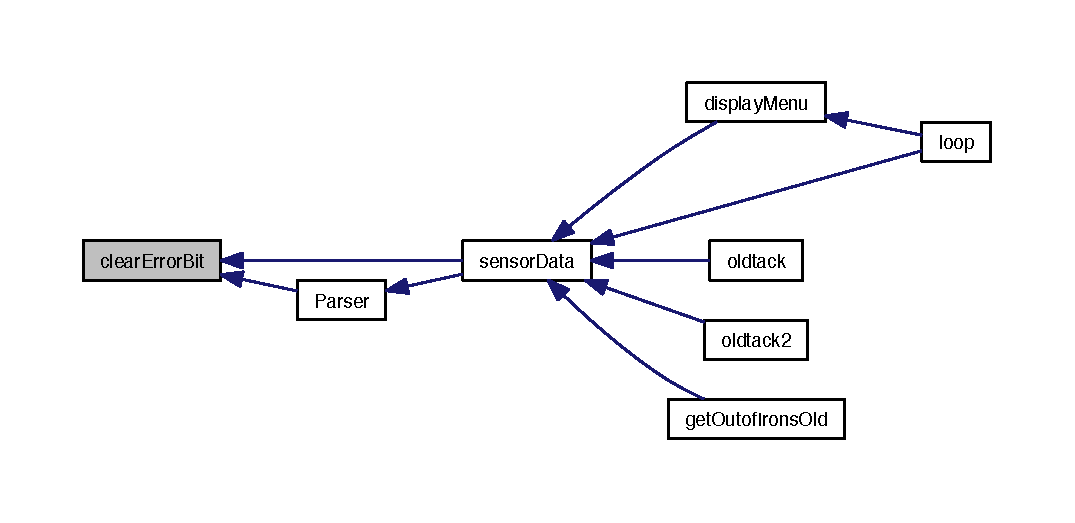
\includegraphics[width=350pt]{_data_acquisition_8pde_a6e69d0b8b4d3517b8abba6d50cd3b8d0_icgraph}
\end{center}
\end{figure}


\hypertarget{_data_acquisition_8pde_a5e6370de6e960ff592044b790015ba48}{
\index{\-Data\-Acquisition.\-pde@{\-Data\-Acquisition.\-pde}!sensor\-Data@{sensor\-Data}}
\index{sensor\-Data@{sensor\-Data}!DataAcquisition.pde@{\-Data\-Acquisition.\-pde}}
\subsubsection[{sensor\-Data}]{\setlength{\rightskip}{0pt plus 5cm}void sensor\-Data (
\begin{DoxyParamCaption}
\item[{int}]{buffer\-Length, }
\item[{char}]{device}
\end{DoxyParamCaption}
)}}
\label{_data_acquisition_8pde_a5e6370de6e960ff592044b790015ba48}


\-Definition at line 4 of file \-Data\-Acquisition.\-pde.



\-Here is the call graph for this function\-:\nopagebreak
\begin{figure}[H]
\begin{center}
\leavevmode
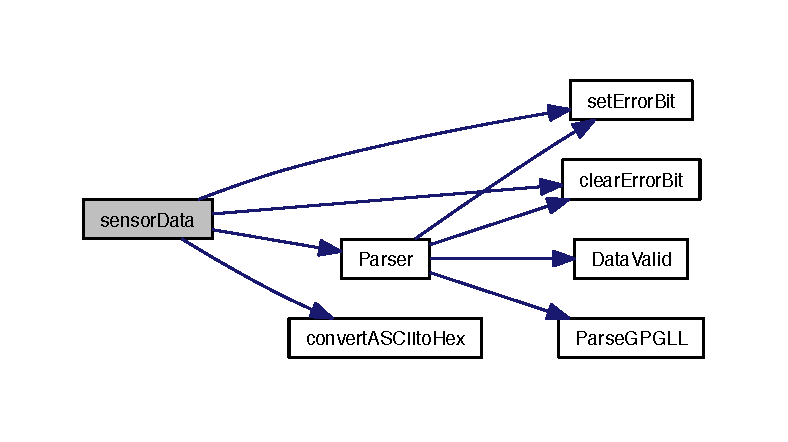
\includegraphics[width=350pt]{_data_acquisition_8pde_a5e6370de6e960ff592044b790015ba48_cgraph}
\end{center}
\end{figure}




\-Here is the caller graph for this function\-:\nopagebreak
\begin{figure}[H]
\begin{center}
\leavevmode
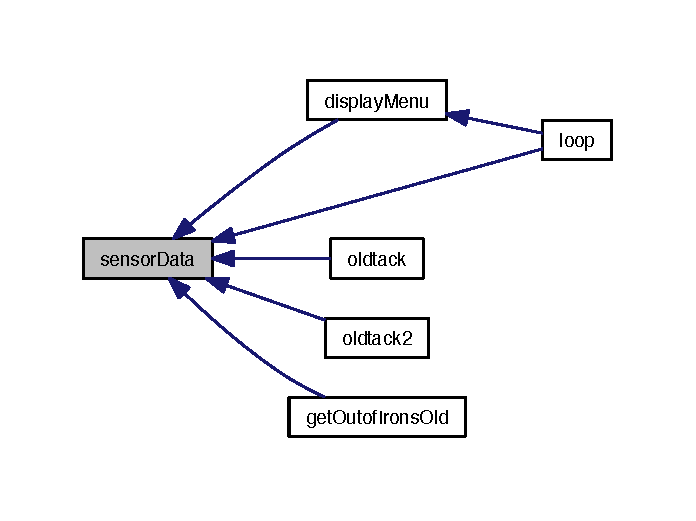
\includegraphics[width=334pt]{_data_acquisition_8pde_a5e6370de6e960ff592044b790015ba48_icgraph}
\end{center}
\end{figure}


\hypertarget{_data_acquisition_8pde_a7754ceed7ff85b4abd95a6ada7828b3d}{
\index{\-Data\-Acquisition.\-pde@{\-Data\-Acquisition.\-pde}!set\-Error\-Bit@{set\-Error\-Bit}}
\index{set\-Error\-Bit@{set\-Error\-Bit}!DataAcquisition.pde@{\-Data\-Acquisition.\-pde}}
\subsubsection[{set\-Error\-Bit}]{\setlength{\rightskip}{0pt plus 5cm}void set\-Error\-Bit (
\begin{DoxyParamCaption}
\item[{int}]{a\-Bit}
\end{DoxyParamCaption}
)}}
\label{_data_acquisition_8pde_a7754ceed7ff85b4abd95a6ada7828b3d}


\-Definition at line 203 of file \-Data\-Acquisition.\-pde.



\-Here is the caller graph for this function\-:\nopagebreak
\begin{figure}[H]
\begin{center}
\leavevmode
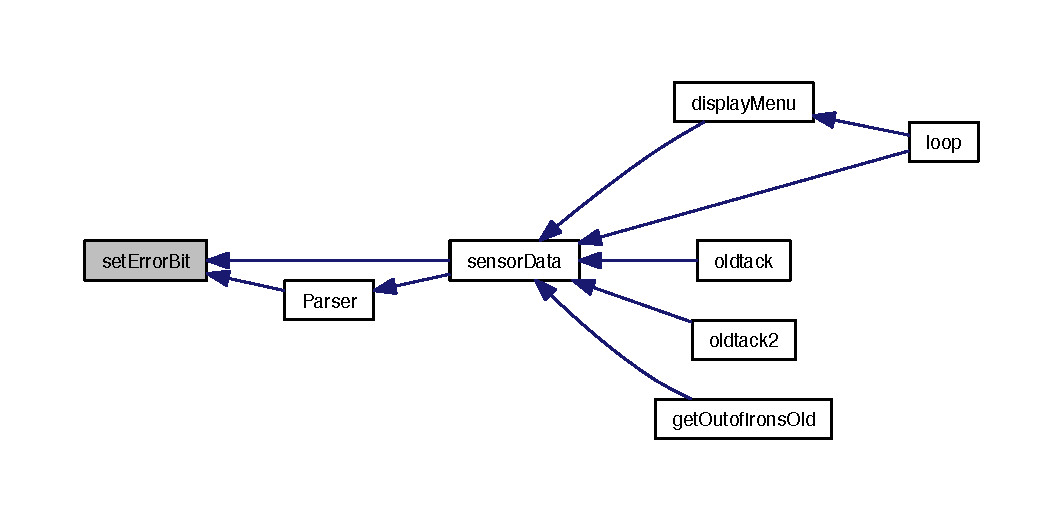
\includegraphics[width=350pt]{_data_acquisition_8pde_a7754ceed7ff85b4abd95a6ada7828b3d_icgraph}
\end{center}
\end{figure}



\hypertarget{_location_struct_8h}{
\section{/\-Users/allgood38/\-Desktop/qmast/sailcode\-\_\-alpha6/\-Location\-Struct.h \-File \-Reference}
\label{_location_struct_8h}\index{/\-Users/allgood38/\-Desktop/qmast/sailcode\-\_\-alpha6/\-Location\-Struct.\-h@{/\-Users/allgood38/\-Desktop/qmast/sailcode\-\_\-alpha6/\-Location\-Struct.\-h}}
}
\-This graph shows which files directly or indirectly include this file\-:\nopagebreak
\begin{figure}[H]
\begin{center}
\leavevmode
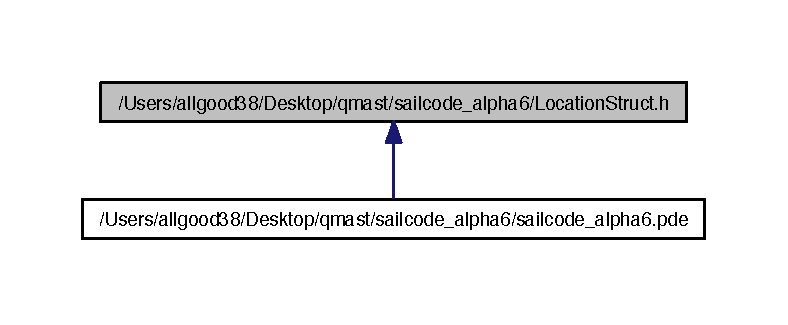
\includegraphics[width=350pt]{_location_struct_8h__dep__incl}
\end{center}
\end{figure}
\subsection*{\-Data \-Structures}
\begin{DoxyCompactItemize}
\item 
struct \hyperlink{structpoints}{points}
\end{DoxyCompactItemize}
\subsection*{\-Variables}
\begin{DoxyCompactItemize}
\item 
\hyperlink{structpoints}{points} \hyperlink{_location_struct_8h_a185b89e8bef2ec3a6ee2768d6c39a9c3}{waypoints} \mbox{[}10\mbox{]}
\item 
\hyperlink{structpoints}{points} \hyperlink{_location_struct_8h_aabb8589a083ce42da76e002537befdda}{station\-Points} \mbox{[}4\mbox{]}
\item 
\hyperlink{structpoints}{points} \hyperlink{_location_struct_8h_a268446ede920c289fe611e02aa0981de}{floating\-Station\-Points} \mbox{[}4\mbox{]}
\item 
\hyperlink{structpoints}{points} \hyperlink{_location_struct_8h_a5836c31336ebde2eb38c5fbc0bee5372}{course\-Points} \mbox{[}10\mbox{]}
\item 
\hyperlink{structpoints}{points} \hyperlink{_location_struct_8h_a2a12b152e09b7f0bbc0d5948b36b5ab4}{clear\-Points}
\item 
\hyperlink{structpoints}{points} \hyperlink{_location_struct_8h_a7101d8f006cf046f26304b4d14474910}{boat\-Location}
\item 
\hyperlink{structpoints}{points} \hyperlink{_location_struct_8h_a2772bf17555c11f8b0d4da815a2fec00}{stay\-Point}
\end{DoxyCompactItemize}


\subsection{\-Variable \-Documentation}
\hypertarget{_location_struct_8h_a7101d8f006cf046f26304b4d14474910}{
\index{\-Location\-Struct.\-h@{\-Location\-Struct.\-h}!boat\-Location@{boat\-Location}}
\index{boat\-Location@{boat\-Location}!LocationStruct.h@{\-Location\-Struct.\-h}}
\subsubsection[{boat\-Location}]{\setlength{\rightskip}{0pt plus 5cm}{\bf points} {\bf boat\-Location}}}
\label{_location_struct_8h_a7101d8f006cf046f26304b4d14474910}


\-Definition at line 35 of file \-Location\-Struct.\-h.

\hypertarget{_location_struct_8h_a2a12b152e09b7f0bbc0d5948b36b5ab4}{
\index{\-Location\-Struct.\-h@{\-Location\-Struct.\-h}!clear\-Points@{clear\-Points}}
\index{clear\-Points@{clear\-Points}!LocationStruct.h@{\-Location\-Struct.\-h}}
\subsubsection[{clear\-Points}]{\setlength{\rightskip}{0pt plus 5cm}{\bf points} {\bf clear\-Points}}}
\label{_location_struct_8h_a2a12b152e09b7f0bbc0d5948b36b5ab4}
{\bfseries \-Initial value\-:}
\begin{DoxyCode}
 {        
  0,0,0,0}
\end{DoxyCode}


\-Definition at line 32 of file \-Location\-Struct.\-h.

\hypertarget{_location_struct_8h_a5836c31336ebde2eb38c5fbc0bee5372}{
\index{\-Location\-Struct.\-h@{\-Location\-Struct.\-h}!course\-Points@{course\-Points}}
\index{course\-Points@{course\-Points}!LocationStruct.h@{\-Location\-Struct.\-h}}
\subsubsection[{course\-Points}]{\setlength{\rightskip}{0pt plus 5cm}{\bf points} {\bf course\-Points}\mbox{[}10\mbox{]}}}
\label{_location_struct_8h_a5836c31336ebde2eb38c5fbc0bee5372}
{\bfseries \-Initial value\-:}
\begin{DoxyCode}
 {
 {0,0,0,0},
 {0,0,0,0},
 {0,0,0,0},
 {0,0,0,0},
 {0,0,0,0},
 {0,0,0,0},
 {0,0,0,0},
 {0,0,0,0},
 {0,0,0,0}}
\end{DoxyCode}


\-Definition at line 21 of file \-Location\-Struct.\-h.

\hypertarget{_location_struct_8h_a268446ede920c289fe611e02aa0981de}{
\index{\-Location\-Struct.\-h@{\-Location\-Struct.\-h}!floating\-Station\-Points@{floating\-Station\-Points}}
\index{floating\-Station\-Points@{floating\-Station\-Points}!LocationStruct.h@{\-Location\-Struct.\-h}}
\subsubsection[{floating\-Station\-Points}]{\setlength{\rightskip}{0pt plus 5cm}{\bf points} {\bf floating\-Station\-Points}\mbox{[}4\mbox{]}}}
\label{_location_struct_8h_a268446ede920c289fe611e02aa0981de}


\-Definition at line 20 of file \-Location\-Struct.\-h.

\hypertarget{_location_struct_8h_aabb8589a083ce42da76e002537befdda}{
\index{\-Location\-Struct.\-h@{\-Location\-Struct.\-h}!station\-Points@{station\-Points}}
\index{station\-Points@{station\-Points}!LocationStruct.h@{\-Location\-Struct.\-h}}
\subsubsection[{station\-Points}]{\setlength{\rightskip}{0pt plus 5cm}{\bf points} {\bf station\-Points}\mbox{[}4\mbox{]}}}
\label{_location_struct_8h_aabb8589a083ce42da76e002537befdda}


\-Definition at line 18 of file \-Location\-Struct.\-h.

\hypertarget{_location_struct_8h_a2772bf17555c11f8b0d4da815a2fec00}{
\index{\-Location\-Struct.\-h@{\-Location\-Struct.\-h}!stay\-Point@{stay\-Point}}
\index{stay\-Point@{stay\-Point}!LocationStruct.h@{\-Location\-Struct.\-h}}
\subsubsection[{stay\-Point}]{\setlength{\rightskip}{0pt plus 5cm}{\bf points} {\bf stay\-Point}}}
\label{_location_struct_8h_a2772bf17555c11f8b0d4da815a2fec00}


\-Definition at line 37 of file \-Location\-Struct.\-h.

\hypertarget{_location_struct_8h_a185b89e8bef2ec3a6ee2768d6c39a9c3}{
\index{\-Location\-Struct.\-h@{\-Location\-Struct.\-h}!waypoints@{waypoints}}
\index{waypoints@{waypoints}!LocationStruct.h@{\-Location\-Struct.\-h}}
\subsubsection[{waypoints}]{\setlength{\rightskip}{0pt plus 5cm}{\bf points} {\bf waypoints}\mbox{[}10\mbox{]}}}
\label{_location_struct_8h_a185b89e8bef2ec3a6ee2768d6c39a9c3}
{\bfseries \-Initial value\-:}
\begin{DoxyCode}
 {        
  {44.0,13.6927,-76.0,-29.5175},       
  {38.0,58.9443,-76.0,-28.7383}, 
  {38.0,58.9515,-76.0,-28.7127}}
\end{DoxyCode}


\-Definition at line 12 of file \-Location\-Struct.\-h.


\hypertarget{_menu_8pde}{
\section{/\-Users/allgood38/\-Desktop/qmast/sailcode\-\_\-alpha6/\-Menu.pde \-File \-Reference}
\label{_menu_8pde}\index{/\-Users/allgood38/\-Desktop/qmast/sailcode\-\_\-alpha6/\-Menu.\-pde@{/\-Users/allgood38/\-Desktop/qmast/sailcode\-\_\-alpha6/\-Menu.\-pde}}
}
\subsection*{\-Functions}
\begin{DoxyCompactItemize}
\item 
int \hyperlink{_menu_8pde_aad9ed7a055a99883645739e4bfca0e5e}{display\-Menu} ()
\end{DoxyCompactItemize}


\subsection{\-Function \-Documentation}
\hypertarget{_menu_8pde_aad9ed7a055a99883645739e4bfca0e5e}{
\index{\-Menu.\-pde@{\-Menu.\-pde}!display\-Menu@{display\-Menu}}
\index{display\-Menu@{display\-Menu}!Menu.pde@{\-Menu.\-pde}}
\subsubsection[{display\-Menu}]{\setlength{\rightskip}{0pt plus 5cm}int display\-Menu (
\begin{DoxyParamCaption}
{}
\end{DoxyParamCaption}
)}}
\label{_menu_8pde_aad9ed7a055a99883645739e4bfca0e5e}


\-Definition at line 1 of file \-Menu.\-pde.



\-Here is the call graph for this function\-:\nopagebreak
\begin{figure}[H]
\begin{center}
\leavevmode
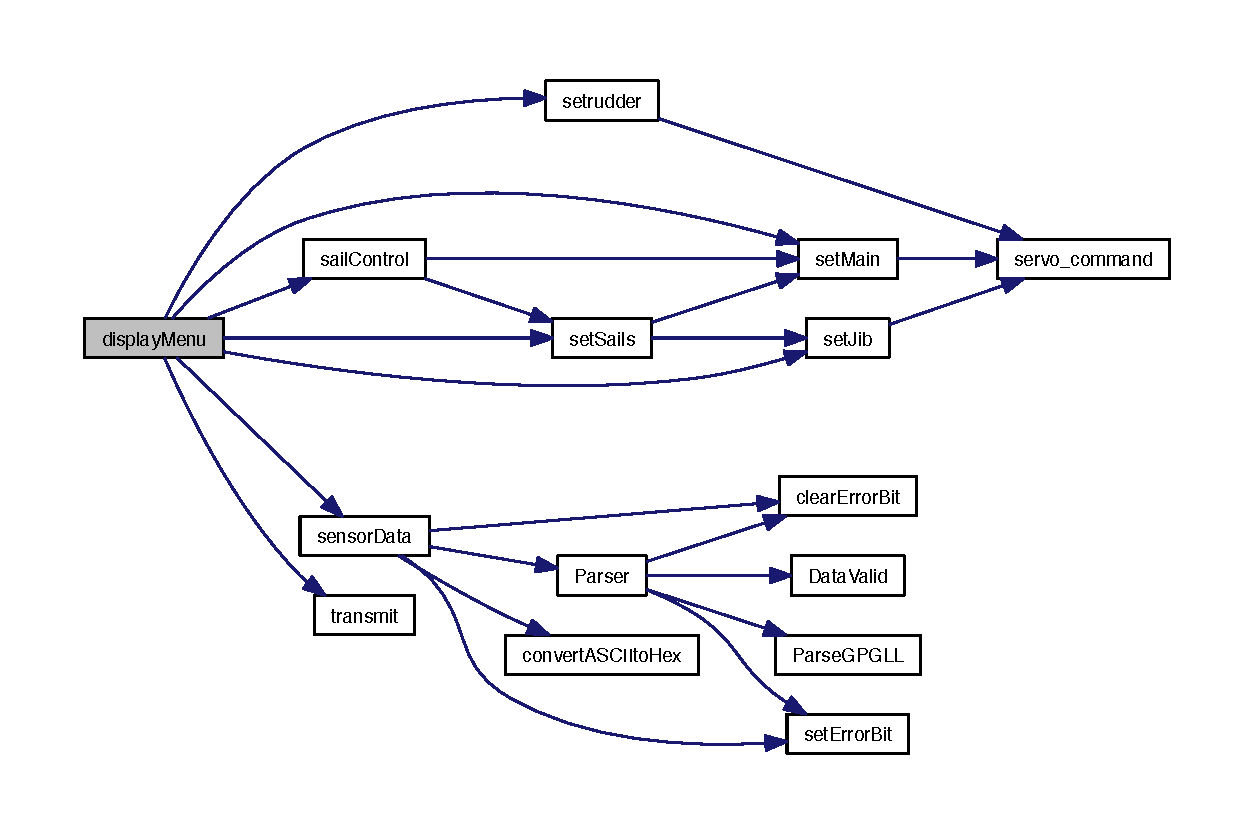
\includegraphics[width=350pt]{_menu_8pde_aad9ed7a055a99883645739e4bfca0e5e_cgraph}
\end{center}
\end{figure}




\-Here is the caller graph for this function\-:\nopagebreak
\begin{figure}[H]
\begin{center}
\leavevmode
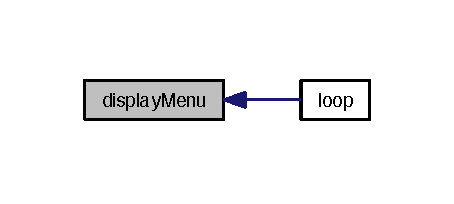
\includegraphics[width=218pt]{_menu_8pde_aad9ed7a055a99883645739e4bfca0e5e_icgraph}
\end{center}
\end{figure}



\hypertarget{_motor_control_functions_8pde}{
\section{/\-Users/allgood38/\-Desktop/qmast/sailcode\-\_\-alpha6/\-Motor\-Control\-Functions.pde \-File \-Reference}
\label{_motor_control_functions_8pde}\index{/\-Users/allgood38/\-Desktop/qmast/sailcode\-\_\-alpha6/\-Motor\-Control\-Functions.\-pde@{/\-Users/allgood38/\-Desktop/qmast/sailcode\-\_\-alpha6/\-Motor\-Control\-Functions.\-pde}}
}
\subsection*{\-Functions}
\begin{DoxyCompactItemize}
\item 
void \hyperlink{_motor_control_functions_8pde_a13167cafd07541f82a26312a556f5a7a}{servo\-\_\-command} (int whichservo, int position, byte long\-Range)
\item 
void \hyperlink{_motor_control_functions_8pde_ada2247ce798f57b0f35794901100c48b}{setrudder} (float ang)
\item 
void \hyperlink{_motor_control_functions_8pde_a3ee6de88bcd944f9cb1b7301769c8b7e}{set\-Sails} (float ang)
\item 
void \hyperlink{_motor_control_functions_8pde_a6e741ed9688f5a70307e8baabab9326a}{set\-Jib} (float ang)
\item 
void \hyperlink{_motor_control_functions_8pde_ab945c39b15584683f123bca1f5df6faa}{set\-Main} (float ang)
\end{DoxyCompactItemize}


\subsection{\-Function \-Documentation}
\hypertarget{_motor_control_functions_8pde_a13167cafd07541f82a26312a556f5a7a}{
\index{\-Motor\-Control\-Functions.\-pde@{\-Motor\-Control\-Functions.\-pde}!servo\-\_\-command@{servo\-\_\-command}}
\index{servo\-\_\-command@{servo\-\_\-command}!MotorControlFunctions.pde@{\-Motor\-Control\-Functions.\-pde}}
\subsubsection[{servo\-\_\-command}]{\setlength{\rightskip}{0pt plus 5cm}void servo\-\_\-command (
\begin{DoxyParamCaption}
\item[{int}]{whichservo, }
\item[{int}]{position, }
\item[{byte}]{long\-Range}
\end{DoxyParamCaption}
)}}
\label{_motor_control_functions_8pde_a13167cafd07541f82a26312a556f5a7a}


\-Definition at line 6 of file \-Motor\-Control\-Functions.\-pde.



\-Here is the caller graph for this function\-:\nopagebreak
\begin{figure}[H]
\begin{center}
\leavevmode
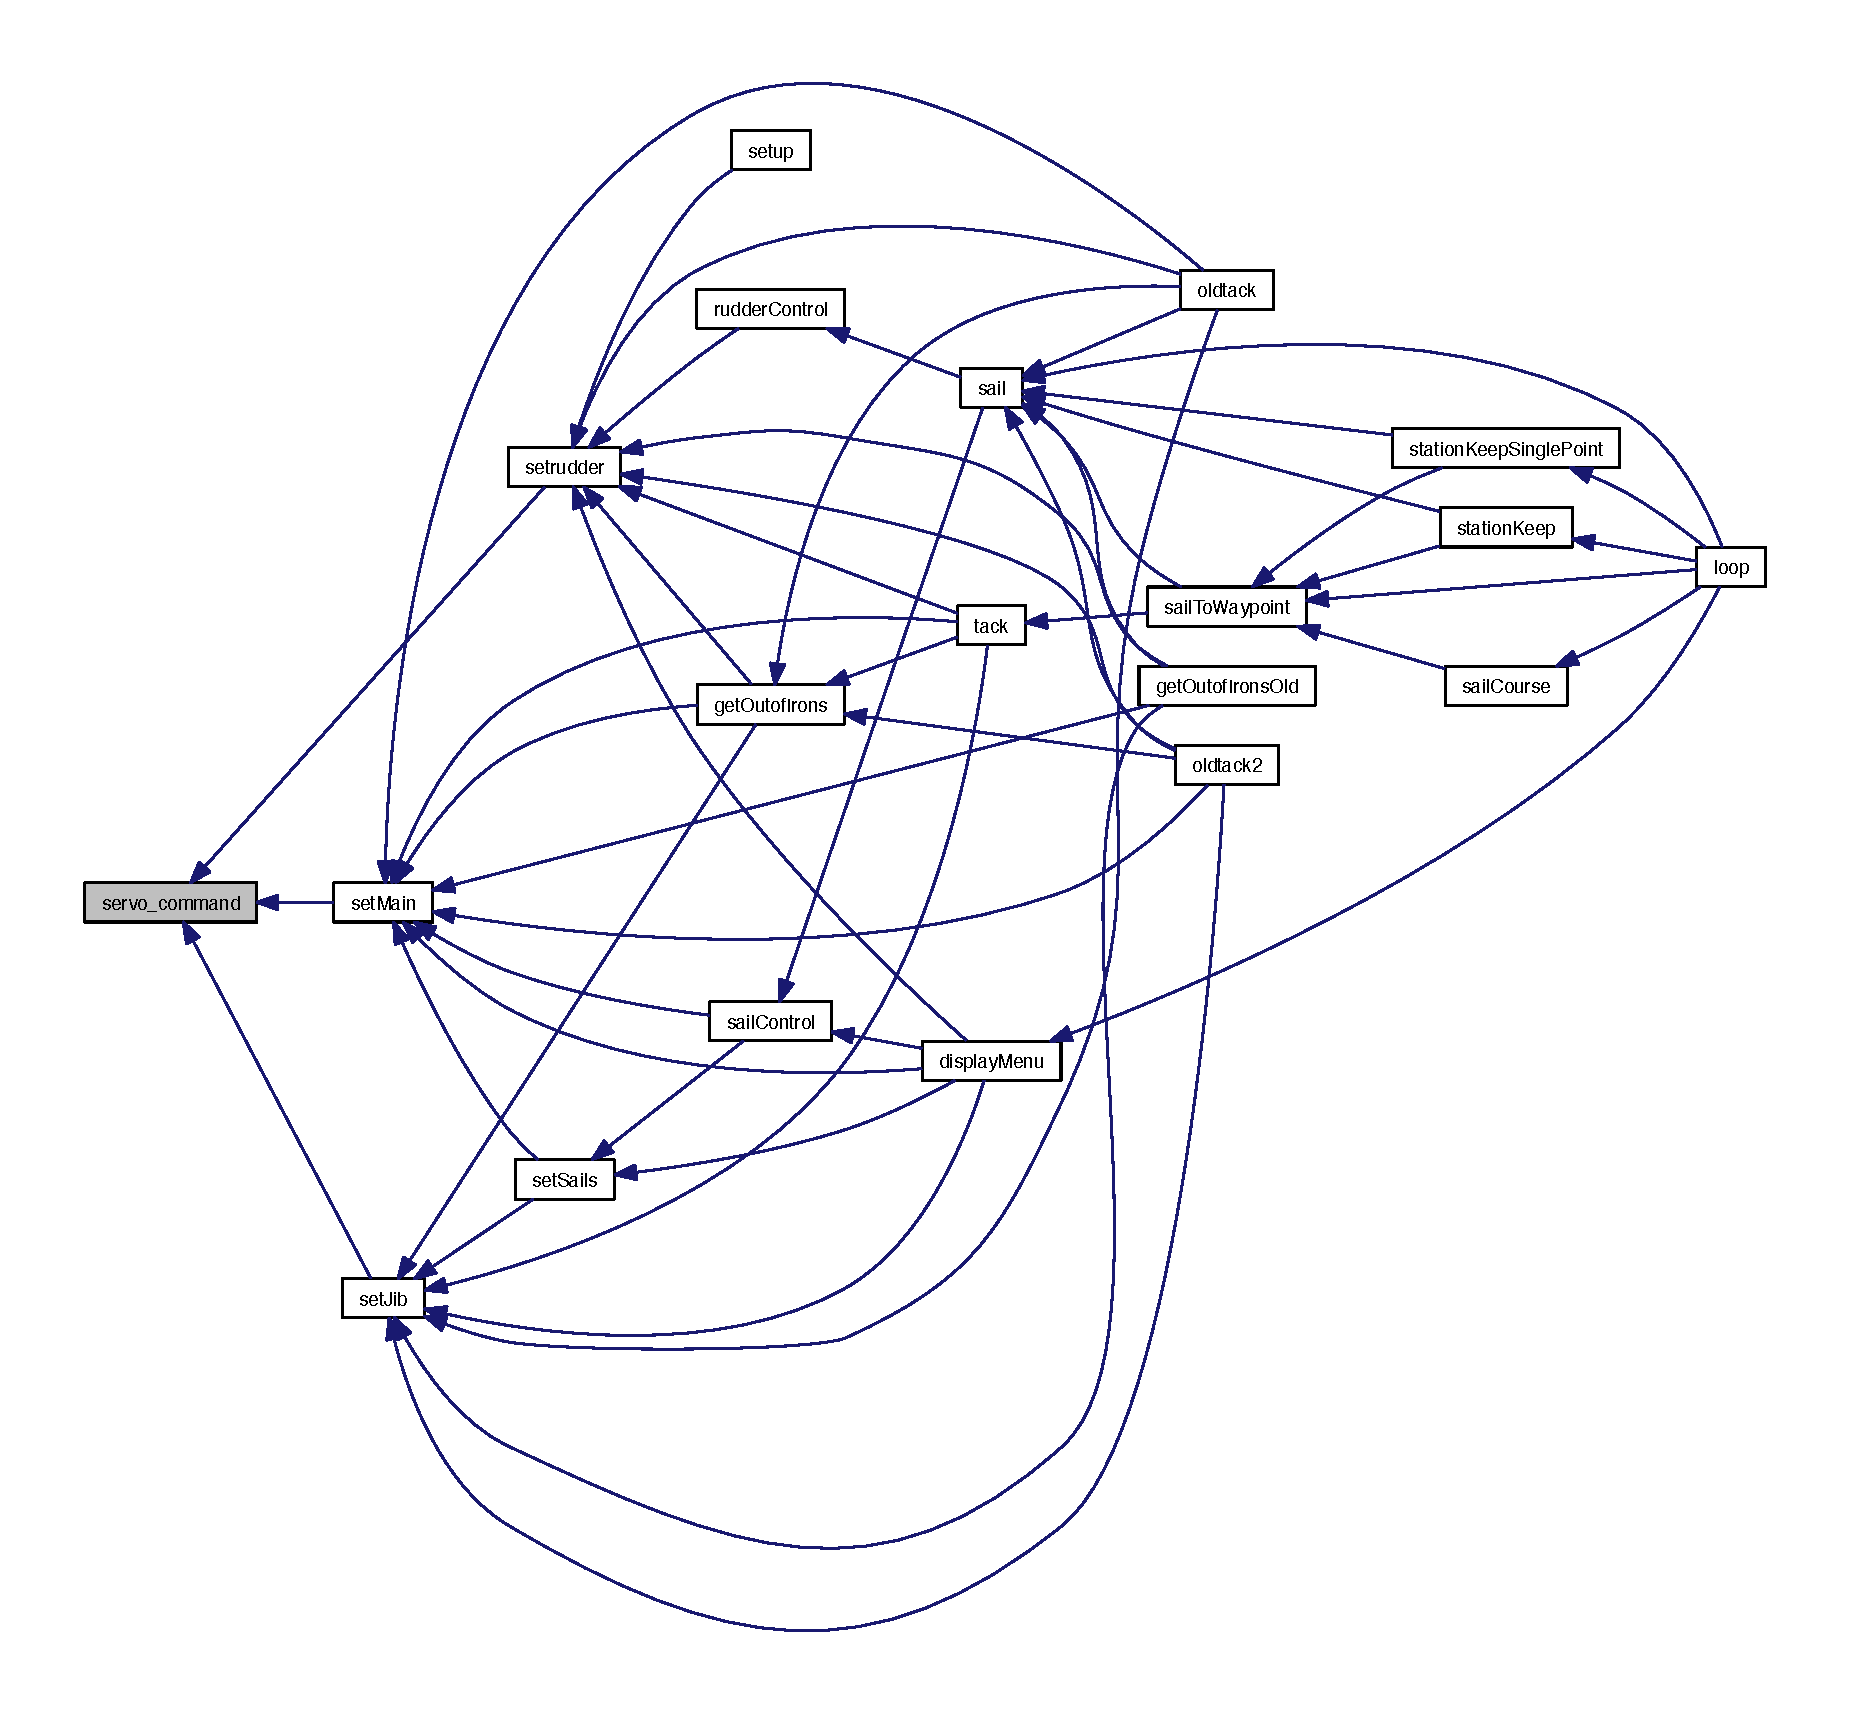
\includegraphics[width=350pt]{_motor_control_functions_8pde_a13167cafd07541f82a26312a556f5a7a_icgraph}
\end{center}
\end{figure}


\hypertarget{_motor_control_functions_8pde_a6e741ed9688f5a70307e8baabab9326a}{
\index{\-Motor\-Control\-Functions.\-pde@{\-Motor\-Control\-Functions.\-pde}!set\-Jib@{set\-Jib}}
\index{set\-Jib@{set\-Jib}!MotorControlFunctions.pde@{\-Motor\-Control\-Functions.\-pde}}
\subsubsection[{set\-Jib}]{\setlength{\rightskip}{0pt plus 5cm}void set\-Jib (
\begin{DoxyParamCaption}
\item[{float}]{ang}
\end{DoxyParamCaption}
)}}
\label{_motor_control_functions_8pde_a6e741ed9688f5a70307e8baabab9326a}


\-Definition at line 37 of file \-Motor\-Control\-Functions.\-pde.



\-Here is the call graph for this function\-:\nopagebreak
\begin{figure}[H]
\begin{center}
\leavevmode
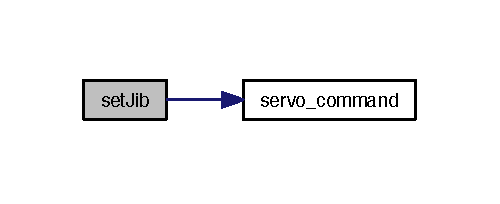
\includegraphics[width=240pt]{_motor_control_functions_8pde_a6e741ed9688f5a70307e8baabab9326a_cgraph}
\end{center}
\end{figure}




\-Here is the caller graph for this function\-:\nopagebreak
\begin{figure}[H]
\begin{center}
\leavevmode
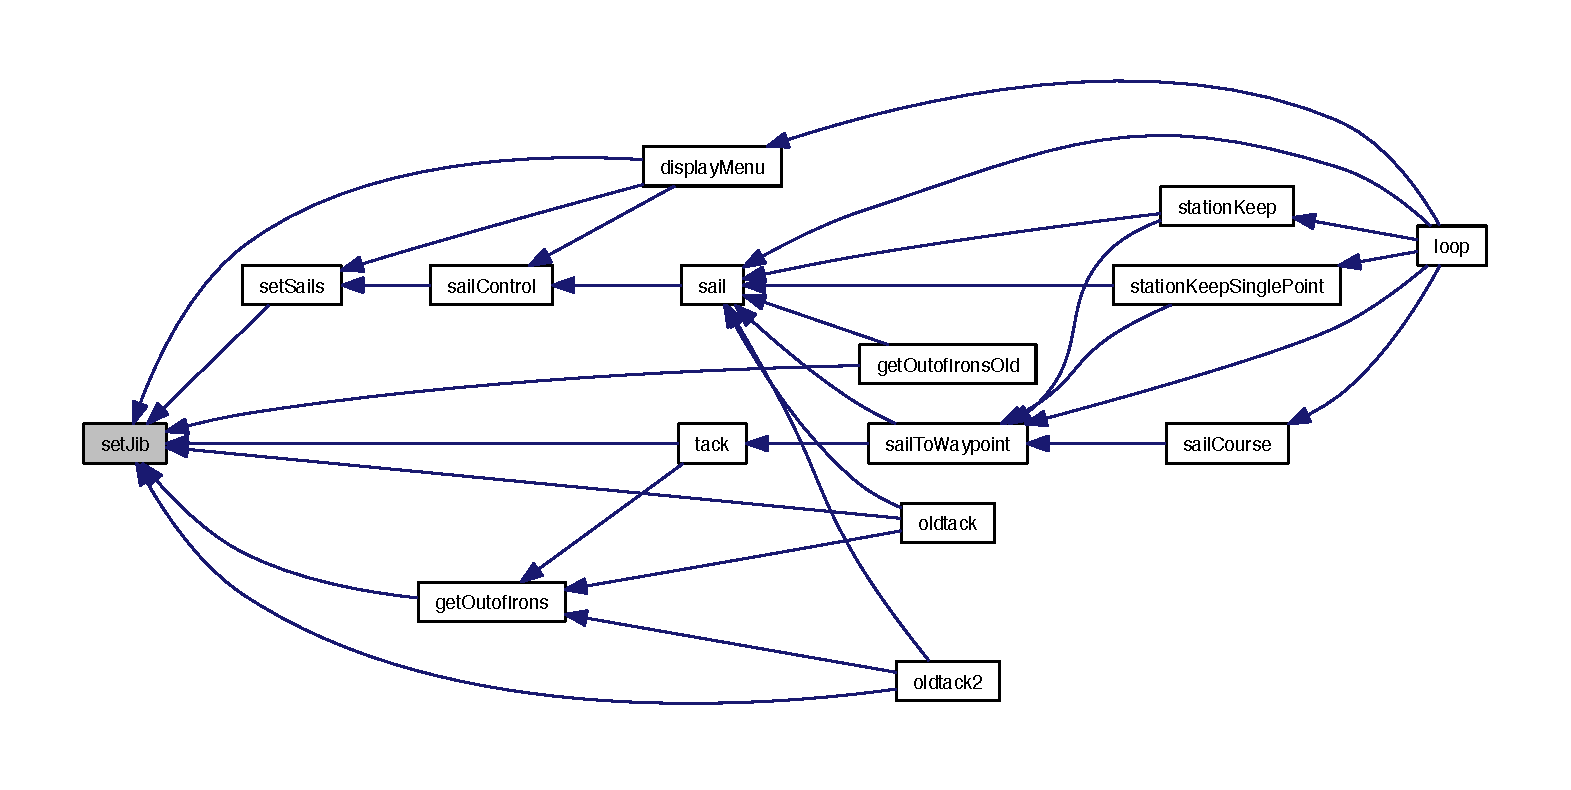
\includegraphics[width=350pt]{_motor_control_functions_8pde_a6e741ed9688f5a70307e8baabab9326a_icgraph}
\end{center}
\end{figure}


\hypertarget{_motor_control_functions_8pde_ab945c39b15584683f123bca1f5df6faa}{
\index{\-Motor\-Control\-Functions.\-pde@{\-Motor\-Control\-Functions.\-pde}!set\-Main@{set\-Main}}
\index{set\-Main@{set\-Main}!MotorControlFunctions.pde@{\-Motor\-Control\-Functions.\-pde}}
\subsubsection[{set\-Main}]{\setlength{\rightskip}{0pt plus 5cm}void set\-Main (
\begin{DoxyParamCaption}
\item[{float}]{ang}
\end{DoxyParamCaption}
)}}
\label{_motor_control_functions_8pde_ab945c39b15584683f123bca1f5df6faa}


\-Definition at line 49 of file \-Motor\-Control\-Functions.\-pde.



\-Here is the call graph for this function\-:\nopagebreak
\begin{figure}[H]
\begin{center}
\leavevmode
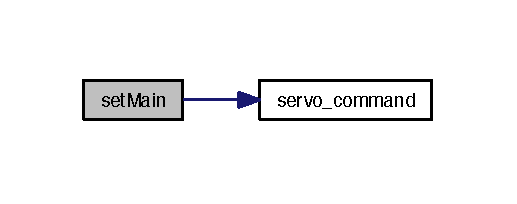
\includegraphics[width=248pt]{_motor_control_functions_8pde_ab945c39b15584683f123bca1f5df6faa_cgraph}
\end{center}
\end{figure}




\-Here is the caller graph for this function\-:\nopagebreak
\begin{figure}[H]
\begin{center}
\leavevmode
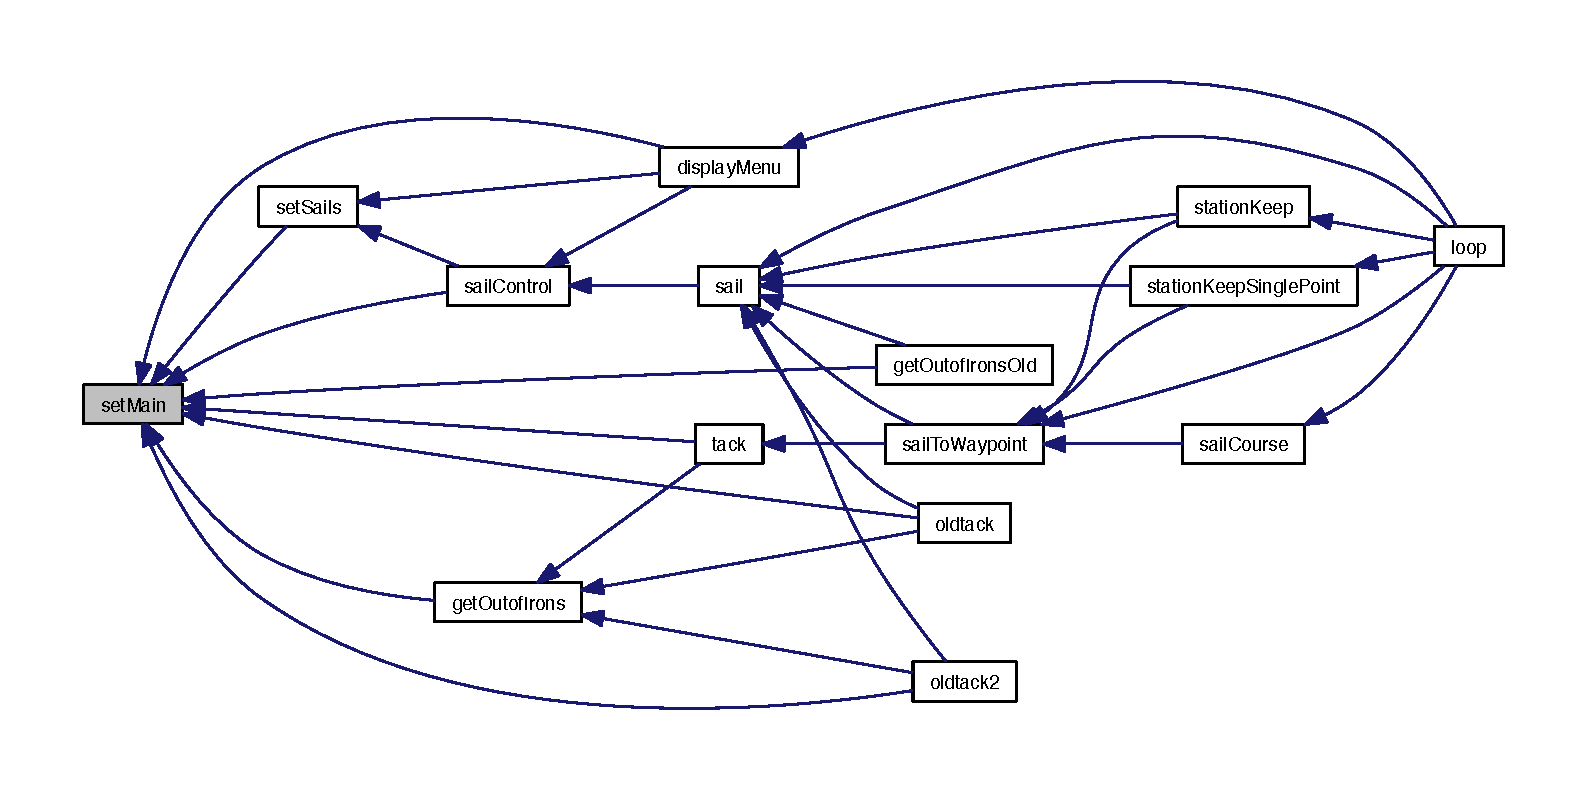
\includegraphics[width=350pt]{_motor_control_functions_8pde_ab945c39b15584683f123bca1f5df6faa_icgraph}
\end{center}
\end{figure}


\hypertarget{_motor_control_functions_8pde_ada2247ce798f57b0f35794901100c48b}{
\index{\-Motor\-Control\-Functions.\-pde@{\-Motor\-Control\-Functions.\-pde}!setrudder@{setrudder}}
\index{setrudder@{setrudder}!MotorControlFunctions.pde@{\-Motor\-Control\-Functions.\-pde}}
\subsubsection[{setrudder}]{\setlength{\rightskip}{0pt plus 5cm}void setrudder (
\begin{DoxyParamCaption}
\item[{float}]{ang}
\end{DoxyParamCaption}
)}}
\label{_motor_control_functions_8pde_ada2247ce798f57b0f35794901100c48b}


\-Definition at line 17 of file \-Motor\-Control\-Functions.\-pde.



\-Here is the call graph for this function\-:\nopagebreak
\begin{figure}[H]
\begin{center}
\leavevmode
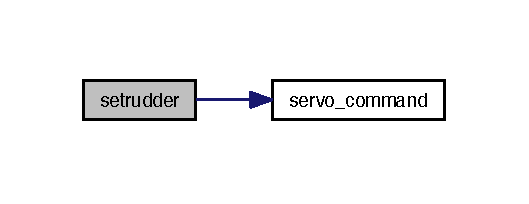
\includegraphics[width=254pt]{_motor_control_functions_8pde_ada2247ce798f57b0f35794901100c48b_cgraph}
\end{center}
\end{figure}




\-Here is the caller graph for this function\-:\nopagebreak
\begin{figure}[H]
\begin{center}
\leavevmode
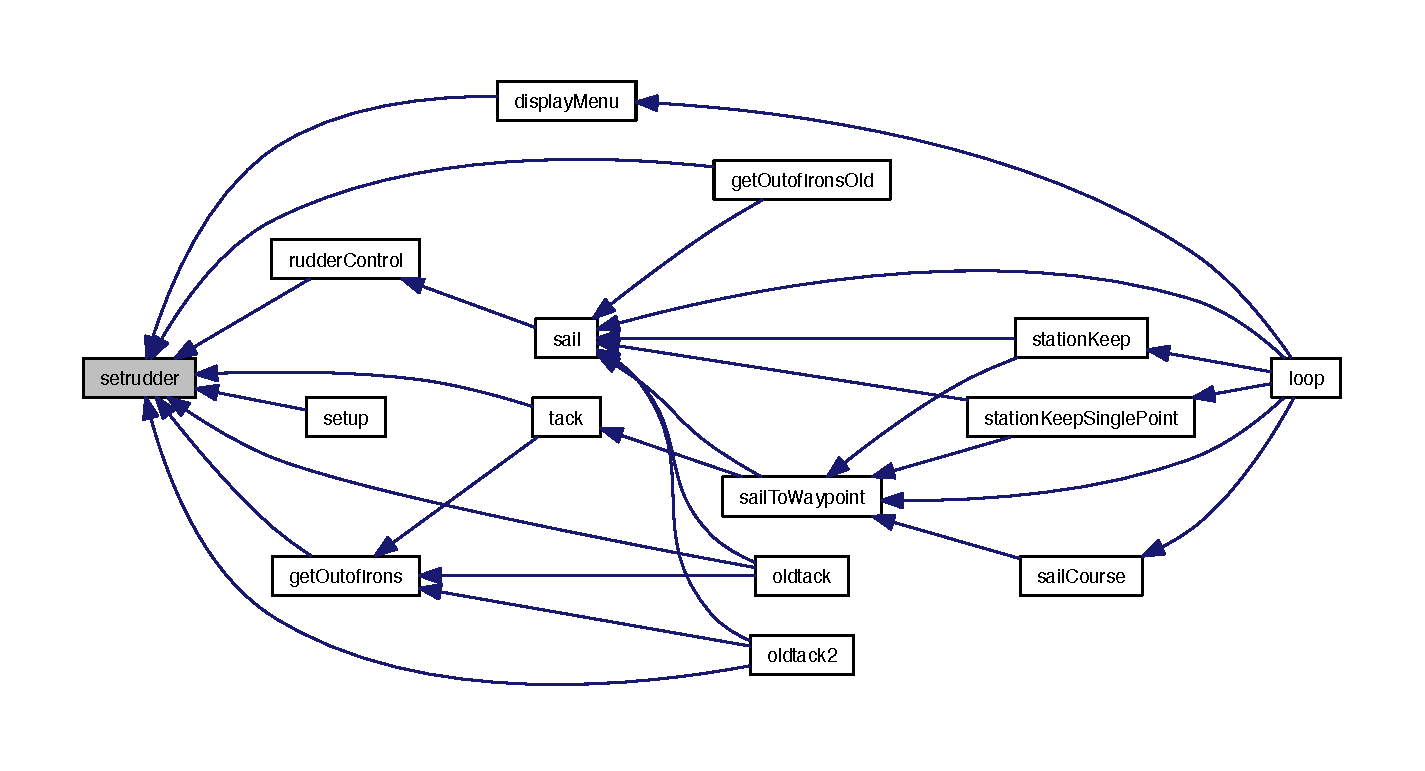
\includegraphics[width=350pt]{_motor_control_functions_8pde_ada2247ce798f57b0f35794901100c48b_icgraph}
\end{center}
\end{figure}


\hypertarget{_motor_control_functions_8pde_a3ee6de88bcd944f9cb1b7301769c8b7e}{
\index{\-Motor\-Control\-Functions.\-pde@{\-Motor\-Control\-Functions.\-pde}!set\-Sails@{set\-Sails}}
\index{set\-Sails@{set\-Sails}!MotorControlFunctions.pde@{\-Motor\-Control\-Functions.\-pde}}
\subsubsection[{set\-Sails}]{\setlength{\rightskip}{0pt plus 5cm}void set\-Sails (
\begin{DoxyParamCaption}
\item[{float}]{ang}
\end{DoxyParamCaption}
)}}
\label{_motor_control_functions_8pde_a3ee6de88bcd944f9cb1b7301769c8b7e}


\-Definition at line 30 of file \-Motor\-Control\-Functions.\-pde.



\-Here is the call graph for this function\-:\nopagebreak
\begin{figure}[H]
\begin{center}
\leavevmode
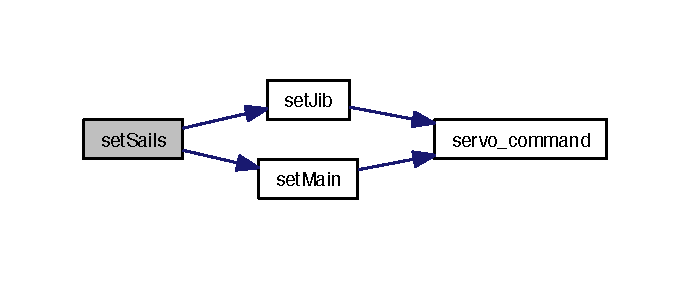
\includegraphics[width=332pt]{_motor_control_functions_8pde_a3ee6de88bcd944f9cb1b7301769c8b7e_cgraph}
\end{center}
\end{figure}




\-Here is the caller graph for this function\-:\nopagebreak
\begin{figure}[H]
\begin{center}
\leavevmode
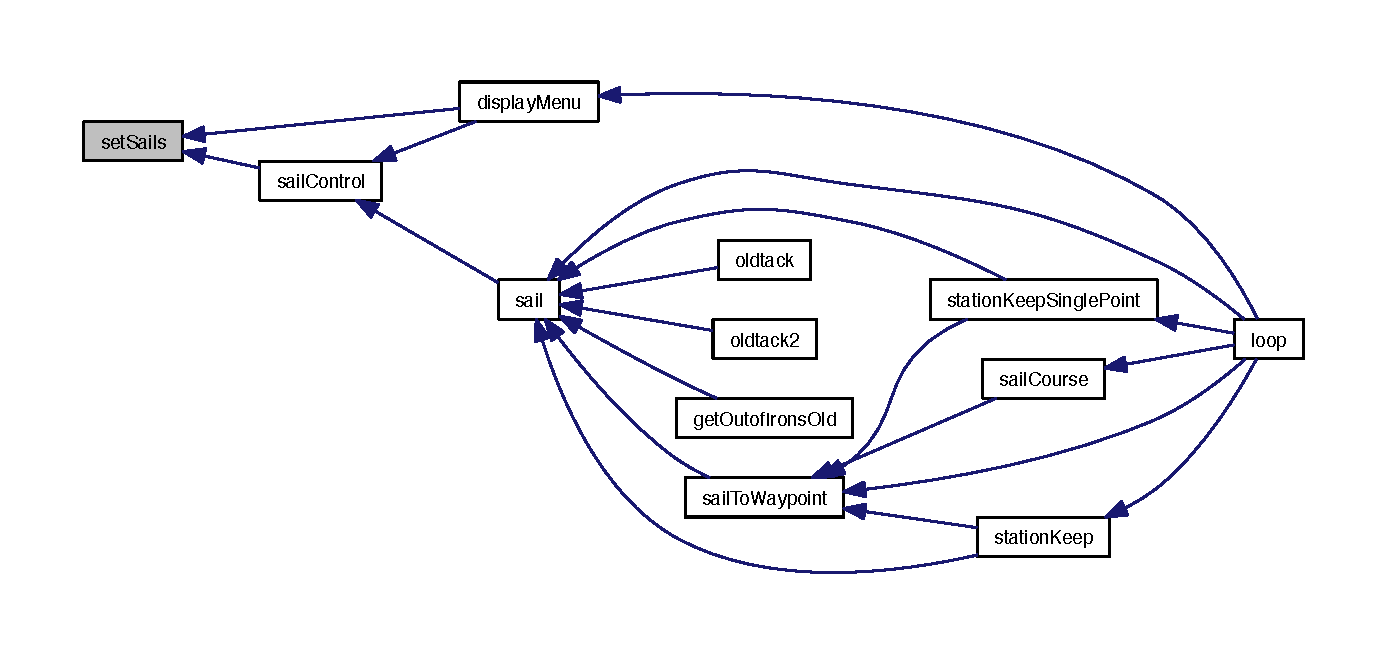
\includegraphics[width=350pt]{_motor_control_functions_8pde_a3ee6de88bcd944f9cb1b7301769c8b7e_icgraph}
\end{center}
\end{figure}



\hypertarget{_navigation_code_8pde}{
\section{/\-Users/allgood38/\-Desktop/qmast/sailcode\-\_\-alpha6/\-Navigation\-Code.pde \-File \-Reference}
\label{_navigation_code_8pde}\index{/\-Users/allgood38/\-Desktop/qmast/sailcode\-\_\-alpha6/\-Navigation\-Code.\-pde@{/\-Users/allgood38/\-Desktop/qmast/sailcode\-\_\-alpha6/\-Navigation\-Code.\-pde}}
}
\subsection*{\-Functions}
\begin{DoxyCompactItemize}
\item 
double \hyperlink{_navigation_code_8pde_a5a81fac76ec3537d65664a394090479f}{\-G\-P\-Sdistance} (struct \hyperlink{structpoints}{points} location1, struct \hyperlink{structpoints}{points} location2)
\item 
int \hyperlink{_navigation_code_8pde_a4fffe1cc3f2386b3364495749dfebc9e}{get\-Waypoint\-Dirn} (struct \hyperlink{structpoints}{points} waypoint)
\item 
int \hyperlink{_navigation_code_8pde_aff425444a43bfea4cccd00c915eff7a5}{get\-Close\-Hauled\-Dirn} ()
\item 
int \hyperlink{_navigation_code_8pde_a30e51ef32f10ba72235e75013d5235b9}{get\-Opposite\-Close\-Hauled\-Dirn} ()
\item 
int \hyperlink{_navigation_code_8pde_ae8999f3c7fe4fd1480b06dd5b60d78f5}{get\-Wind\-Dirn} ()
\end{DoxyCompactItemize}


\subsection{\-Function \-Documentation}
\hypertarget{_navigation_code_8pde_aff425444a43bfea4cccd00c915eff7a5}{
\index{\-Navigation\-Code.\-pde@{\-Navigation\-Code.\-pde}!get\-Close\-Hauled\-Dirn@{get\-Close\-Hauled\-Dirn}}
\index{get\-Close\-Hauled\-Dirn@{get\-Close\-Hauled\-Dirn}!NavigationCode.pde@{\-Navigation\-Code.\-pde}}
\subsubsection[{get\-Close\-Hauled\-Dirn}]{\setlength{\rightskip}{0pt plus 5cm}int get\-Close\-Hauled\-Dirn (
\begin{DoxyParamCaption}
{}
\end{DoxyParamCaption}
)}}
\label{_navigation_code_8pde_aff425444a43bfea4cccd00c915eff7a5}


\-Definition at line 42 of file \-Navigation\-Code.\-pde.



\-Here is the call graph for this function\-:\nopagebreak
\begin{figure}[H]
\begin{center}
\leavevmode
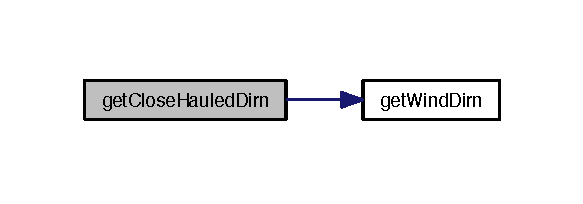
\includegraphics[width=280pt]{_navigation_code_8pde_aff425444a43bfea4cccd00c915eff7a5_cgraph}
\end{center}
\end{figure}




\-Here is the caller graph for this function\-:\nopagebreak
\begin{figure}[H]
\begin{center}
\leavevmode
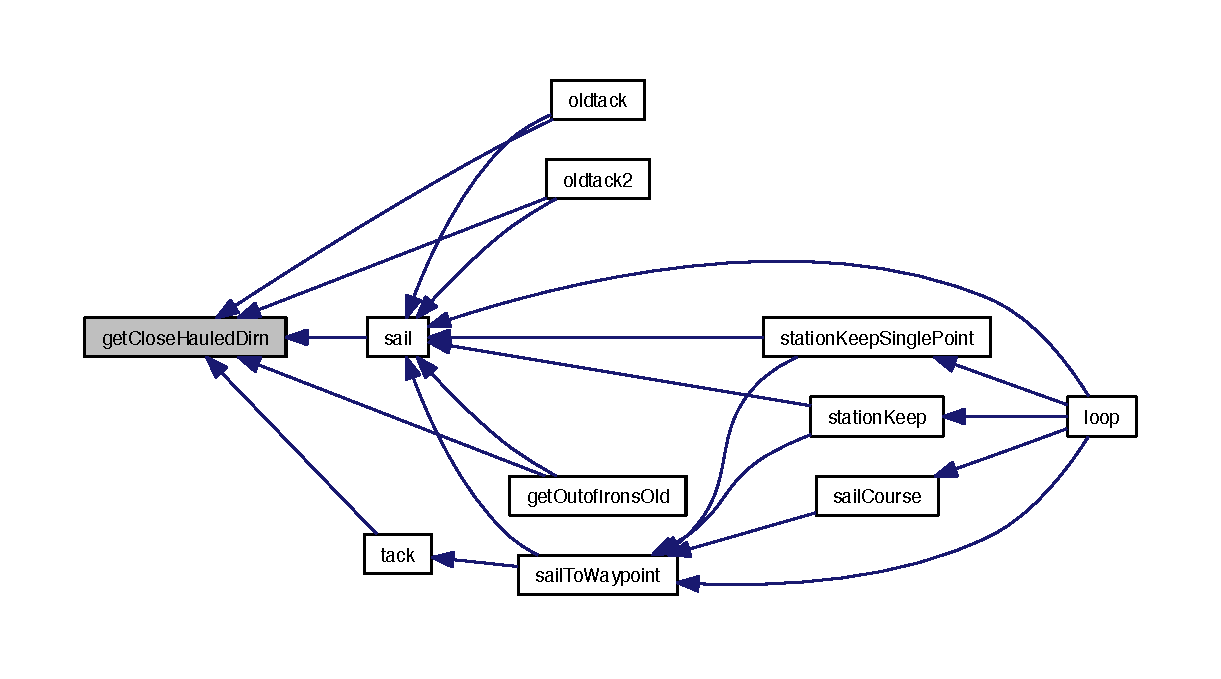
\includegraphics[width=350pt]{_navigation_code_8pde_aff425444a43bfea4cccd00c915eff7a5_icgraph}
\end{center}
\end{figure}


\hypertarget{_navigation_code_8pde_a30e51ef32f10ba72235e75013d5235b9}{
\index{\-Navigation\-Code.\-pde@{\-Navigation\-Code.\-pde}!get\-Opposite\-Close\-Hauled\-Dirn@{get\-Opposite\-Close\-Hauled\-Dirn}}
\index{get\-Opposite\-Close\-Hauled\-Dirn@{get\-Opposite\-Close\-Hauled\-Dirn}!NavigationCode.pde@{\-Navigation\-Code.\-pde}}
\subsubsection[{get\-Opposite\-Close\-Hauled\-Dirn}]{\setlength{\rightskip}{0pt plus 5cm}int get\-Opposite\-Close\-Hauled\-Dirn (
\begin{DoxyParamCaption}
{}
\end{DoxyParamCaption}
)}}
\label{_navigation_code_8pde_a30e51ef32f10ba72235e75013d5235b9}


\-Definition at line 60 of file \-Navigation\-Code.\-pde.



\-Here is the call graph for this function\-:\nopagebreak
\begin{figure}[H]
\begin{center}
\leavevmode
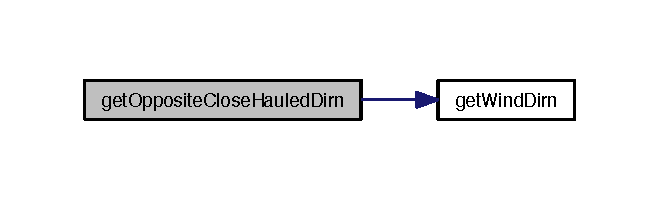
\includegraphics[width=316pt]{_navigation_code_8pde_a30e51ef32f10ba72235e75013d5235b9_cgraph}
\end{center}
\end{figure}


\hypertarget{_navigation_code_8pde_a4fffe1cc3f2386b3364495749dfebc9e}{
\index{\-Navigation\-Code.\-pde@{\-Navigation\-Code.\-pde}!get\-Waypoint\-Dirn@{get\-Waypoint\-Dirn}}
\index{get\-Waypoint\-Dirn@{get\-Waypoint\-Dirn}!NavigationCode.pde@{\-Navigation\-Code.\-pde}}
\subsubsection[{get\-Waypoint\-Dirn}]{\setlength{\rightskip}{0pt plus 5cm}int get\-Waypoint\-Dirn (
\begin{DoxyParamCaption}
\item[{struct {\bf points}}]{waypoint}
\end{DoxyParamCaption}
)}}
\label{_navigation_code_8pde_a4fffe1cc3f2386b3364495749dfebc9e}


\-Definition at line 16 of file \-Navigation\-Code.\-pde.



\-Here is the call graph for this function\-:\nopagebreak
\begin{figure}[H]
\begin{center}
\leavevmode
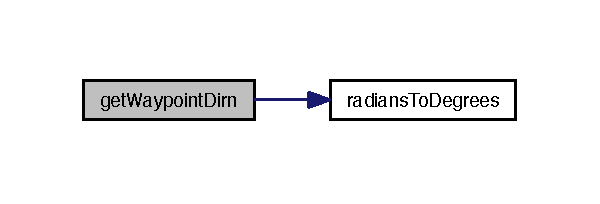
\includegraphics[width=288pt]{_navigation_code_8pde_a4fffe1cc3f2386b3364495749dfebc9e_cgraph}
\end{center}
\end{figure}




\-Here is the caller graph for this function\-:\nopagebreak
\begin{figure}[H]
\begin{center}
\leavevmode
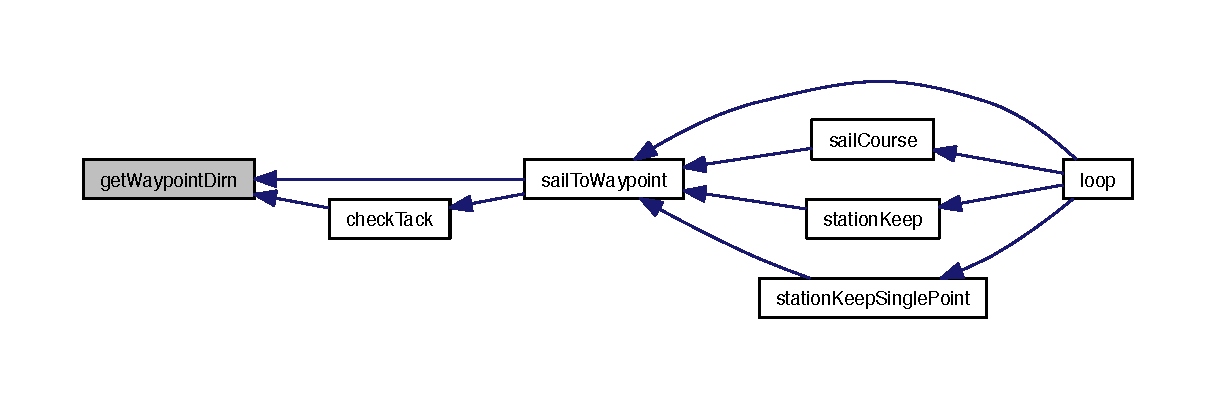
\includegraphics[width=350pt]{_navigation_code_8pde_a4fffe1cc3f2386b3364495749dfebc9e_icgraph}
\end{center}
\end{figure}


\hypertarget{_navigation_code_8pde_ae8999f3c7fe4fd1480b06dd5b60d78f5}{
\index{\-Navigation\-Code.\-pde@{\-Navigation\-Code.\-pde}!get\-Wind\-Dirn@{get\-Wind\-Dirn}}
\index{get\-Wind\-Dirn@{get\-Wind\-Dirn}!NavigationCode.pde@{\-Navigation\-Code.\-pde}}
\subsubsection[{get\-Wind\-Dirn}]{\setlength{\rightskip}{0pt plus 5cm}int get\-Wind\-Dirn (
\begin{DoxyParamCaption}
{}
\end{DoxyParamCaption}
)}}
\label{_navigation_code_8pde_ae8999f3c7fe4fd1480b06dd5b60d78f5}


\-Definition at line 83 of file \-Navigation\-Code.\-pde.



\-Here is the caller graph for this function\-:\nopagebreak
\begin{figure}[H]
\begin{center}
\leavevmode
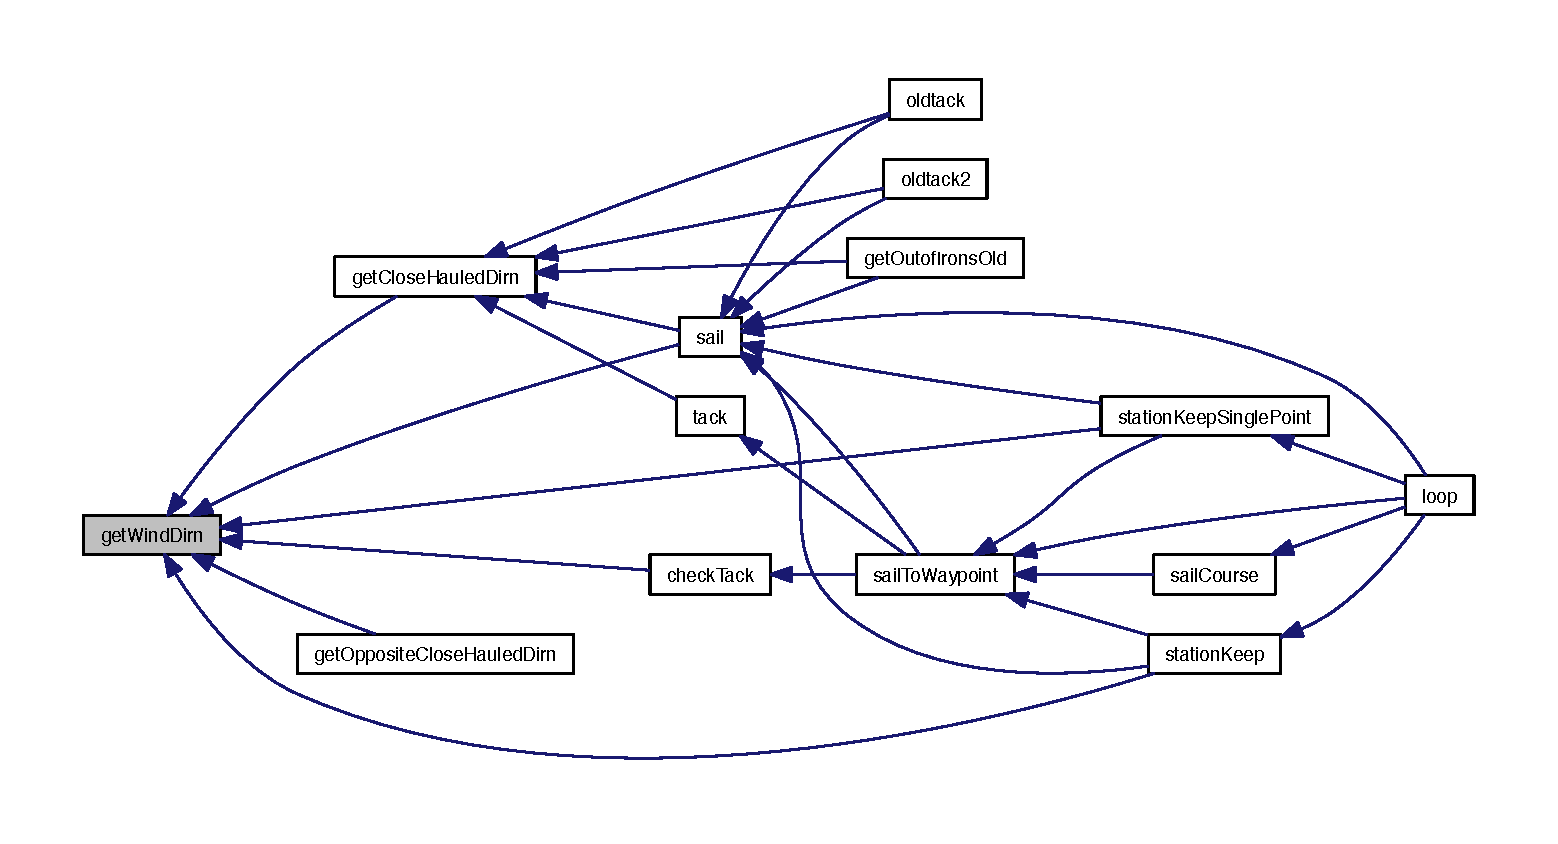
\includegraphics[width=350pt]{_navigation_code_8pde_ae8999f3c7fe4fd1480b06dd5b60d78f5_icgraph}
\end{center}
\end{figure}


\hypertarget{_navigation_code_8pde_a5a81fac76ec3537d65664a394090479f}{
\index{\-Navigation\-Code.\-pde@{\-Navigation\-Code.\-pde}!\-G\-P\-Sdistance@{\-G\-P\-Sdistance}}
\index{\-G\-P\-Sdistance@{\-G\-P\-Sdistance}!NavigationCode.pde@{\-Navigation\-Code.\-pde}}
\subsubsection[{\-G\-P\-Sdistance}]{\setlength{\rightskip}{0pt plus 5cm}double \-G\-P\-Sdistance (
\begin{DoxyParamCaption}
\item[{struct {\bf points}}]{location1, }
\item[{struct {\bf points}}]{location2}
\end{DoxyParamCaption}
)}}
\label{_navigation_code_8pde_a5a81fac76ec3537d65664a394090479f}


\-Definition at line 1 of file \-Navigation\-Code.\-pde.



\-Here is the caller graph for this function\-:\nopagebreak
\begin{figure}[H]
\begin{center}
\leavevmode
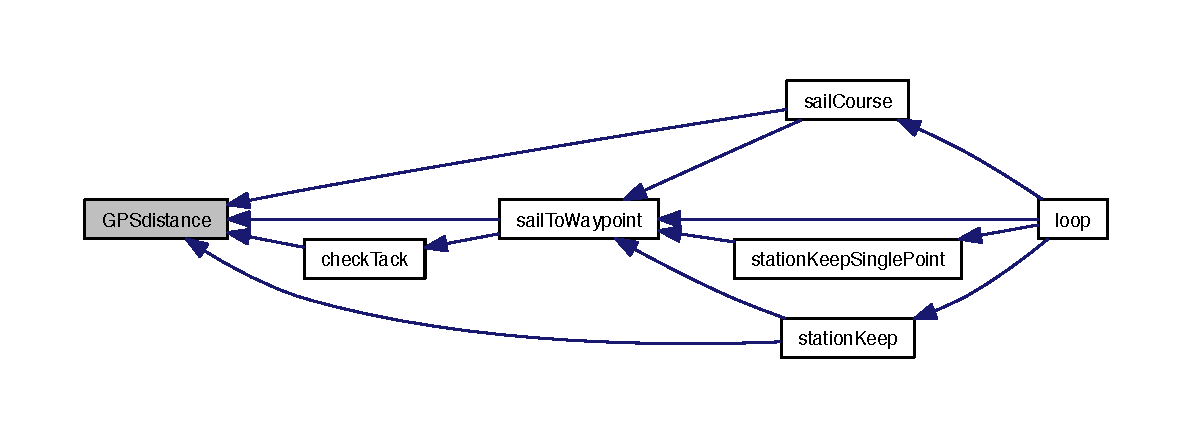
\includegraphics[width=350pt]{_navigation_code_8pde_a5a81fac76ec3537d65664a394090479f_icgraph}
\end{center}
\end{figure}



\hypertarget{oldtack_8pde}{
\section{/\-Users/allgood38/\-Desktop/qmast/sailcode\-\_\-alpha6/oldtack.pde \-File \-Reference}
\label{oldtack_8pde}\index{/\-Users/allgood38/\-Desktop/qmast/sailcode\-\_\-alpha6/oldtack.\-pde@{/\-Users/allgood38/\-Desktop/qmast/sailcode\-\_\-alpha6/oldtack.\-pde}}
}
\subsection*{\-Functions}
\begin{DoxyCompactItemize}
\item 
void \hyperlink{oldtack_8pde_aa56b9f04ea7c8c58f7a0030db9e58925}{oldtack} ()
\item 
void \hyperlink{oldtack_8pde_a4785198fa045d7d139a5e682ac809e62}{oldtack2} ()
\begin{DoxyCompactList}\small\item\em newer revision \end{DoxyCompactList}\item 
void \hyperlink{oldtack_8pde_a30dbce327552d96d2630fed7ec47bfe9}{get\-Outof\-Irons\-Old} (int tackside)
\end{DoxyCompactItemize}


\subsection{\-Function \-Documentation}
\hypertarget{oldtack_8pde_a30dbce327552d96d2630fed7ec47bfe9}{
\index{oldtack.\-pde@{oldtack.\-pde}!get\-Outof\-Irons\-Old@{get\-Outof\-Irons\-Old}}
\index{get\-Outof\-Irons\-Old@{get\-Outof\-Irons\-Old}!oldtack.pde@{oldtack.\-pde}}
\subsubsection[{get\-Outof\-Irons\-Old}]{\setlength{\rightskip}{0pt plus 5cm}void get\-Outof\-Irons\-Old (
\begin{DoxyParamCaption}
\item[{int}]{tackside}
\end{DoxyParamCaption}
)}}
\label{oldtack_8pde_a30dbce327552d96d2630fed7ec47bfe9}


\-Definition at line 171 of file oldtack.\-pde.



\-Here is the call graph for this function\-:\nopagebreak
\begin{figure}[H]
\begin{center}
\leavevmode
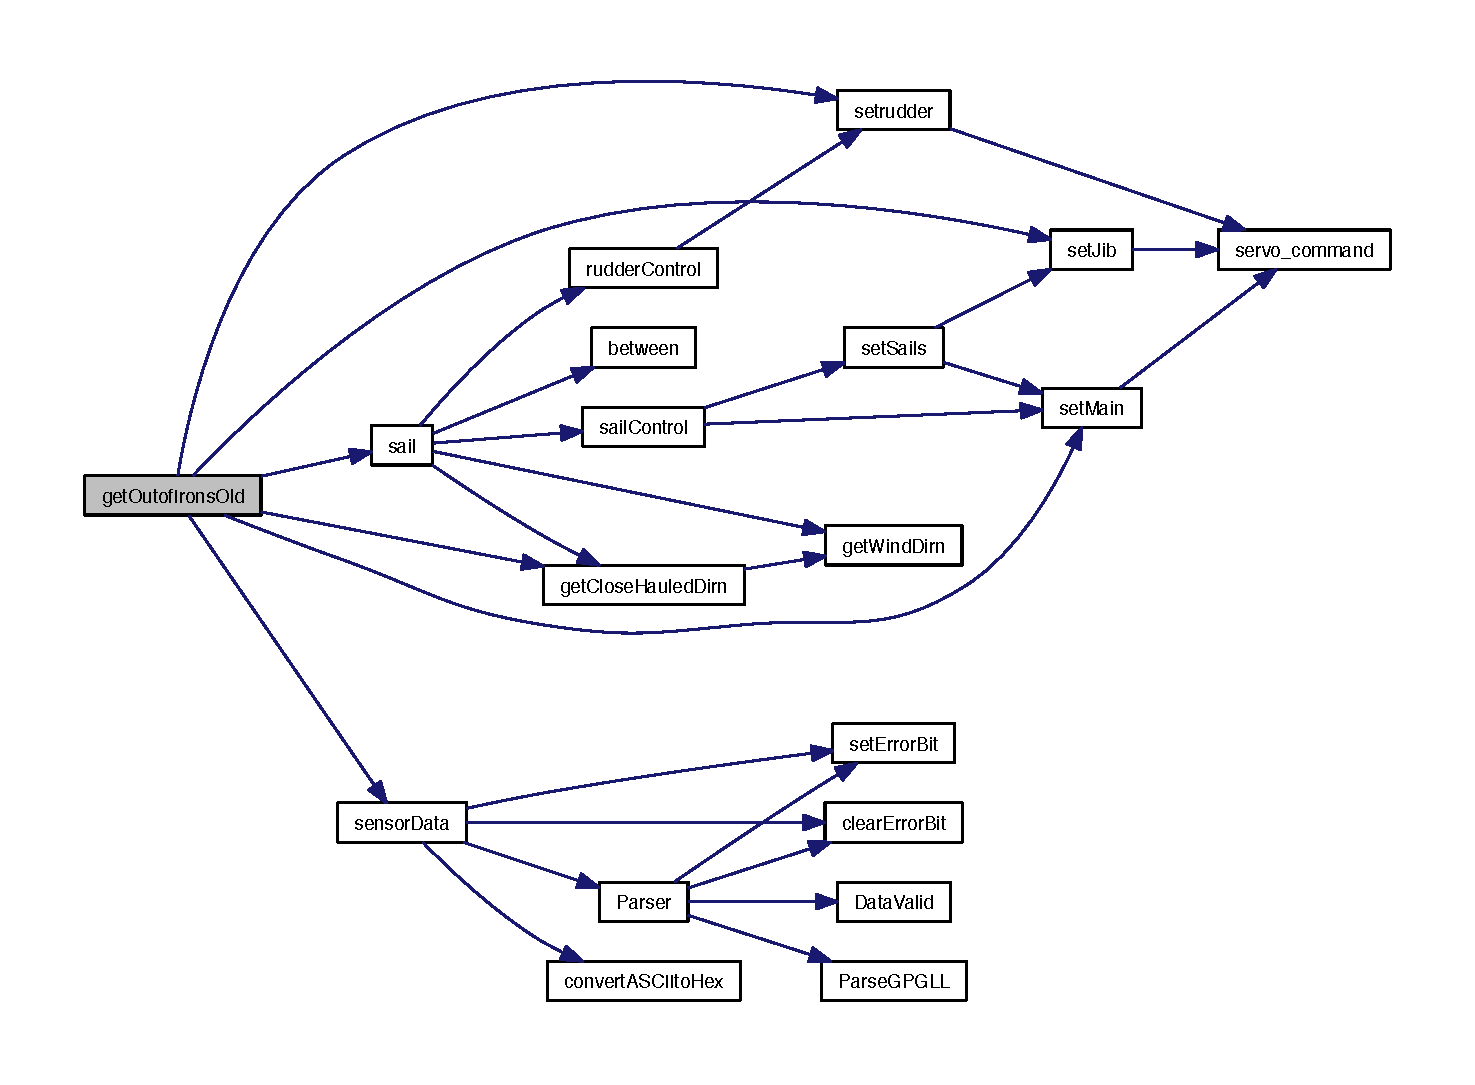
\includegraphics[width=350pt]{oldtack_8pde_a30dbce327552d96d2630fed7ec47bfe9_cgraph}
\end{center}
\end{figure}


\hypertarget{oldtack_8pde_aa56b9f04ea7c8c58f7a0030db9e58925}{
\index{oldtack.\-pde@{oldtack.\-pde}!oldtack@{oldtack}}
\index{oldtack@{oldtack}!oldtack.pde@{oldtack.\-pde}}
\subsubsection[{oldtack}]{\setlength{\rightskip}{0pt plus 5cm}void oldtack (
\begin{DoxyParamCaption}
{}
\end{DoxyParamCaption}
)}}
\label{oldtack_8pde_aa56b9f04ea7c8c58f7a0030db9e58925}


\-Definition at line 6 of file oldtack.\-pde.



\-Here is the call graph for this function\-:\nopagebreak
\begin{figure}[H]
\begin{center}
\leavevmode
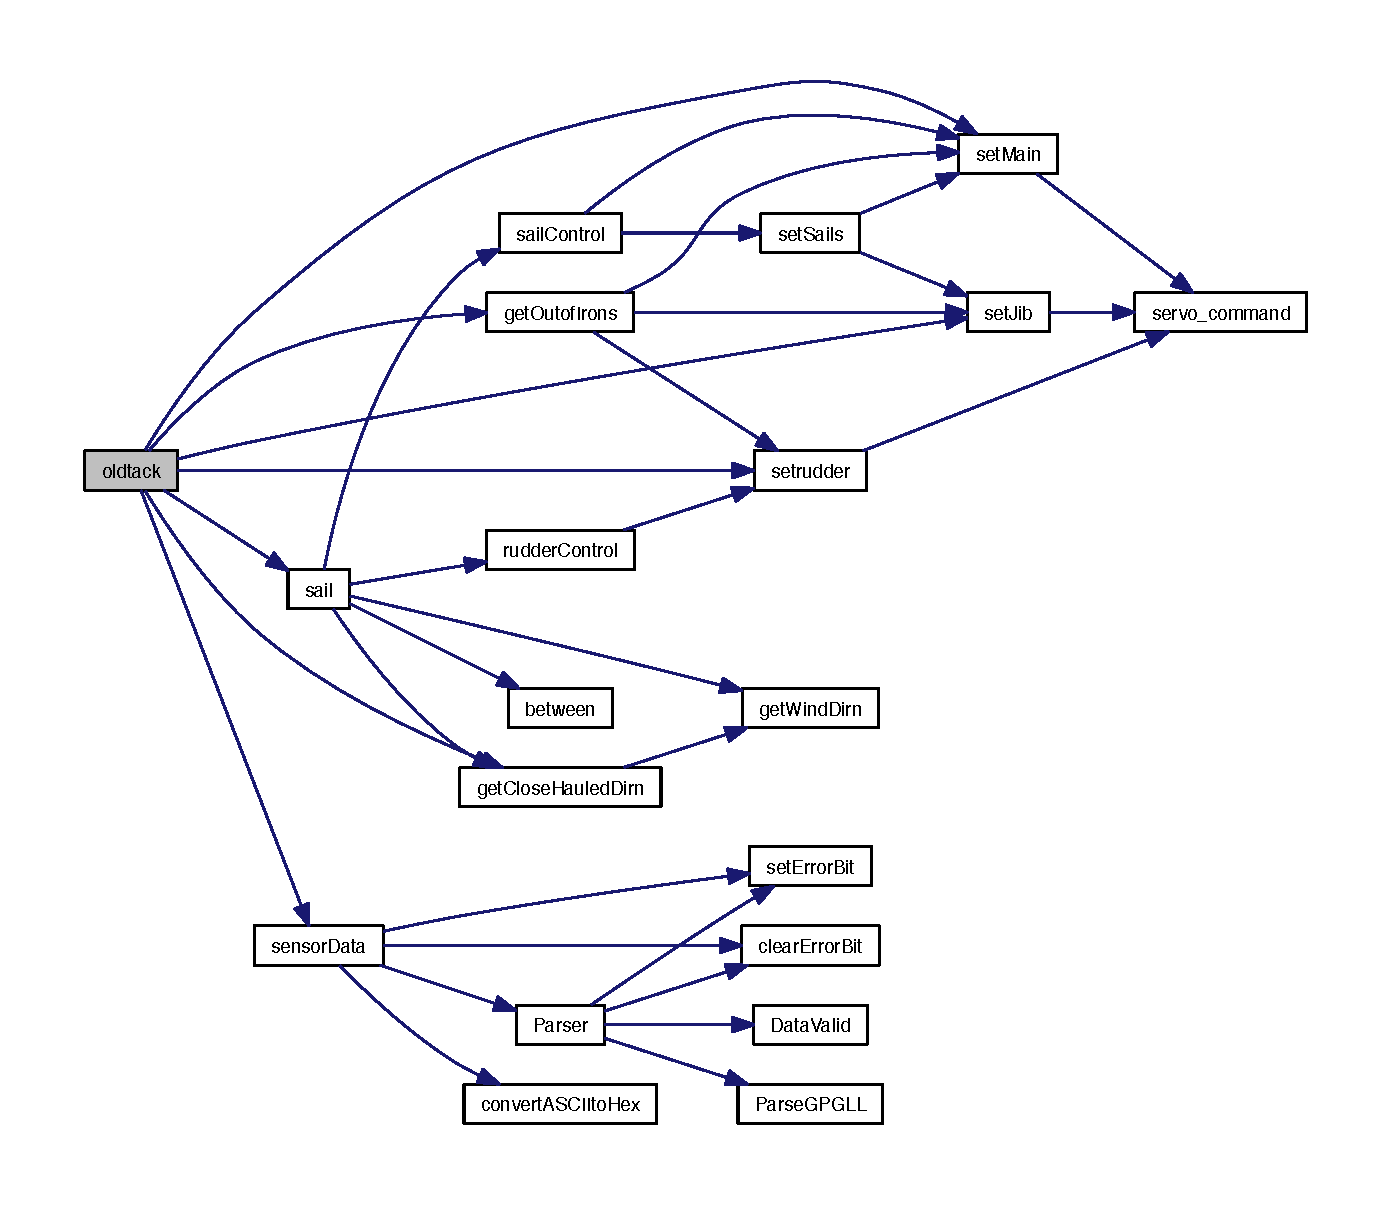
\includegraphics[width=350pt]{oldtack_8pde_aa56b9f04ea7c8c58f7a0030db9e58925_cgraph}
\end{center}
\end{figure}


\hypertarget{oldtack_8pde_a4785198fa045d7d139a5e682ac809e62}{
\index{oldtack.\-pde@{oldtack.\-pde}!oldtack2@{oldtack2}}
\index{oldtack2@{oldtack2}!oldtack.pde@{oldtack.\-pde}}
\subsubsection[{oldtack2}]{\setlength{\rightskip}{0pt plus 5cm}void oldtack2 (
\begin{DoxyParamCaption}
{}
\end{DoxyParamCaption}
)}}
\label{oldtack_8pde_a4785198fa045d7d139a5e682ac809e62}


newer revision 



\-Definition at line 83 of file oldtack.\-pde.



\-Here is the call graph for this function\-:\nopagebreak
\begin{figure}[H]
\begin{center}
\leavevmode
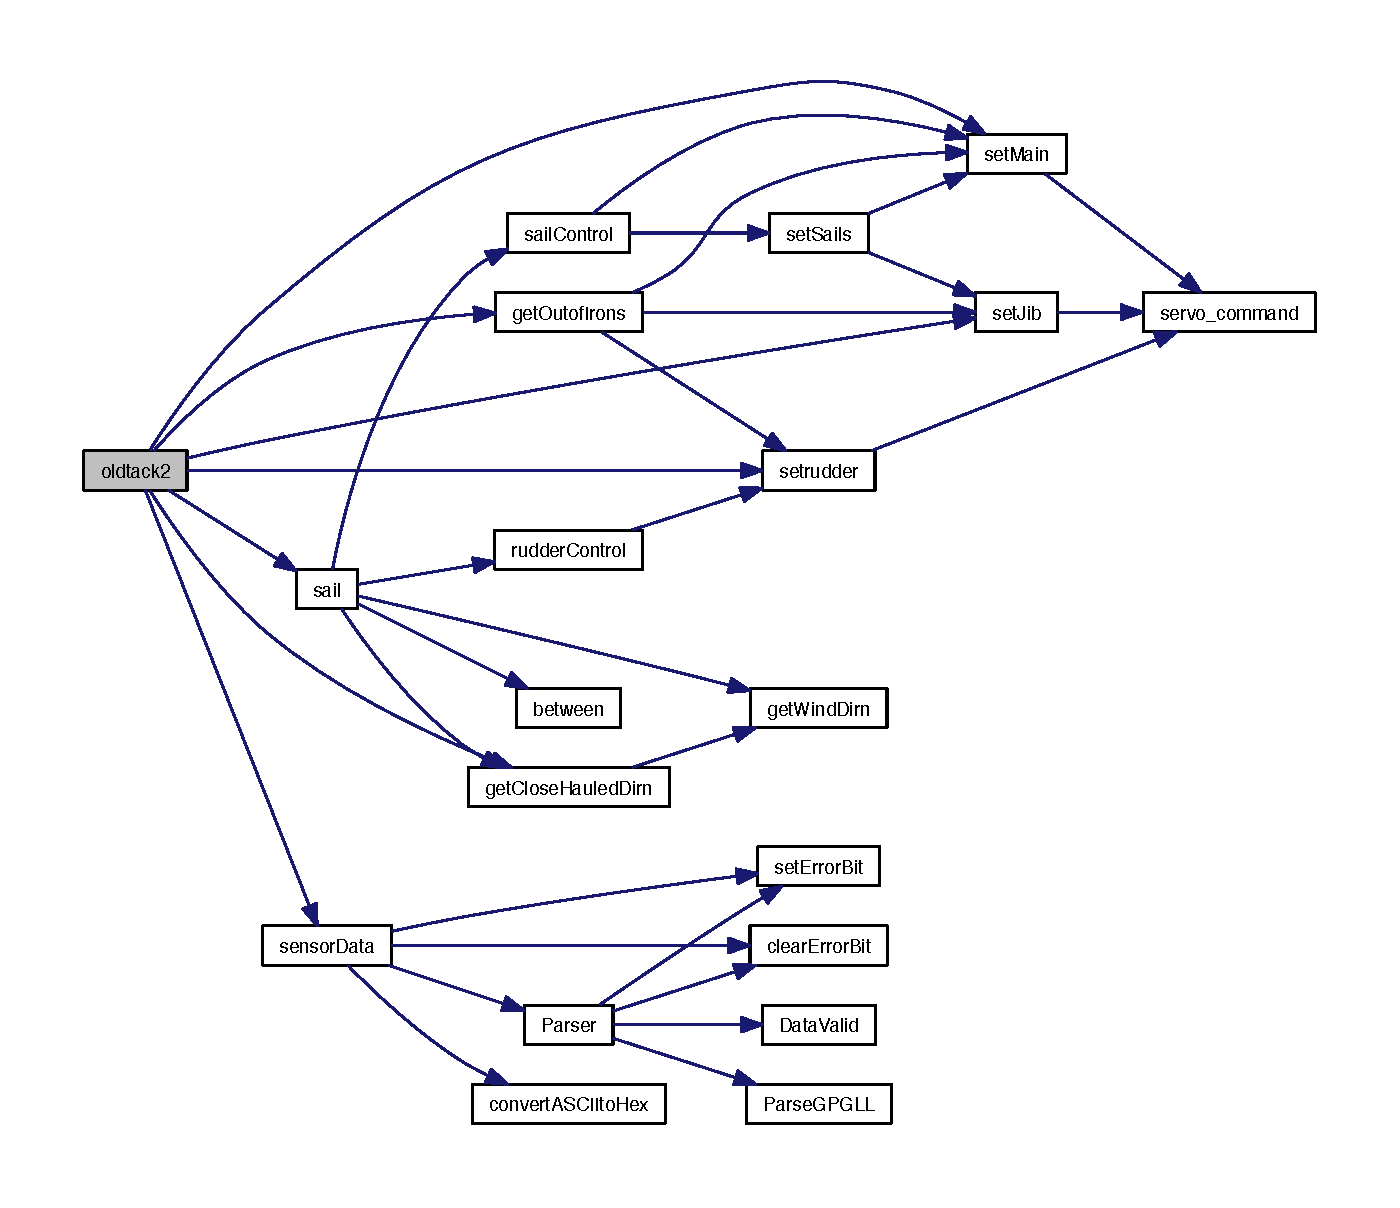
\includegraphics[width=350pt]{oldtack_8pde_a4785198fa045d7d139a5e682ac809e62_cgraph}
\end{center}
\end{figure}



\hypertarget{_parsing_functions_8pde}{
\section{/\-Users/allgood38/\-Desktop/qmast/sailcode\-\_\-alpha6/\-Parsing\-Functions.pde \-File \-Reference}
\label{_parsing_functions_8pde}\index{/\-Users/allgood38/\-Desktop/qmast/sailcode\-\_\-alpha6/\-Parsing\-Functions.\-pde@{/\-Users/allgood38/\-Desktop/qmast/sailcode\-\_\-alpha6/\-Parsing\-Functions.\-pde}}
}
\subsection*{\-Functions}
\begin{DoxyCompactItemize}
\item 
int \hyperlink{_parsing_functions_8pde_adba7fa397be479bf3c2b345e05969c10}{\-Data\-Valid} (char $\ast$val)
\item 
void \hyperlink{_parsing_functions_8pde_a601e25d1a7636238ce5083c54461a17f}{\-Parse\-G\-P\-G\-L\-L} (char $\ast$\-G\-P\-G\-L\-L\-\_\-string, double $\ast$degree, double $\ast$minute)
\item 
int \hyperlink{_parsing_functions_8pde_a9cf045f6db34fd4e2388047fe8045294}{\-Parser} (char $\ast$val)
\end{DoxyCompactItemize}


\subsection{\-Function \-Documentation}
\hypertarget{_parsing_functions_8pde_adba7fa397be479bf3c2b345e05969c10}{
\index{\-Parsing\-Functions.\-pde@{\-Parsing\-Functions.\-pde}!\-Data\-Valid@{\-Data\-Valid}}
\index{\-Data\-Valid@{\-Data\-Valid}!ParsingFunctions.pde@{\-Parsing\-Functions.\-pde}}
\subsubsection[{\-Data\-Valid}]{\setlength{\rightskip}{0pt plus 5cm}int \-Data\-Valid (
\begin{DoxyParamCaption}
\item[{char $\ast$}]{val}
\end{DoxyParamCaption}
)}}
\label{_parsing_functions_8pde_adba7fa397be479bf3c2b345e05969c10}


\-Definition at line 5 of file \-Parsing\-Functions.\-pde.



\-Here is the caller graph for this function\-:\nopagebreak
\begin{figure}[H]
\begin{center}
\leavevmode
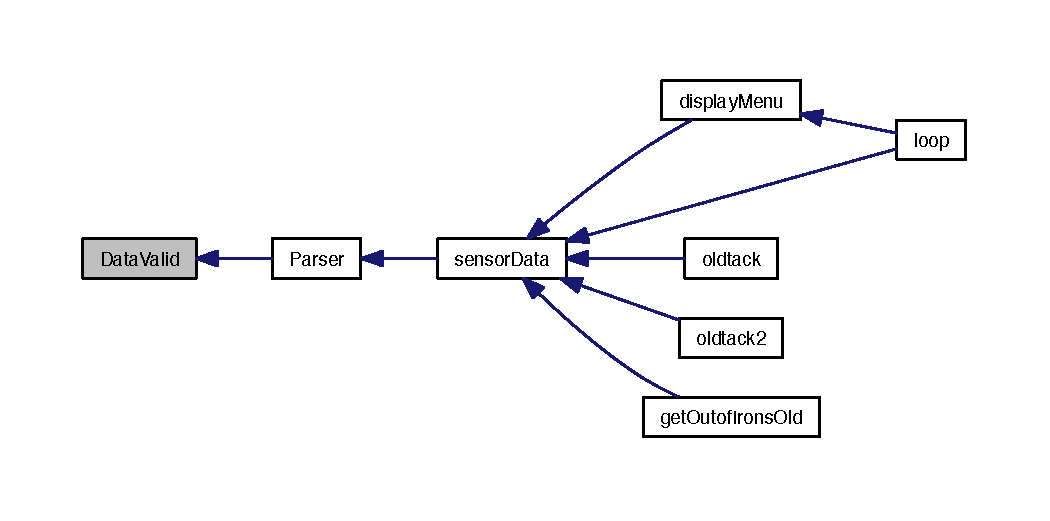
\includegraphics[width=350pt]{_parsing_functions_8pde_adba7fa397be479bf3c2b345e05969c10_icgraph}
\end{center}
\end{figure}


\hypertarget{_parsing_functions_8pde_a601e25d1a7636238ce5083c54461a17f}{
\index{\-Parsing\-Functions.\-pde@{\-Parsing\-Functions.\-pde}!\-Parse\-G\-P\-G\-L\-L@{\-Parse\-G\-P\-G\-L\-L}}
\index{\-Parse\-G\-P\-G\-L\-L@{\-Parse\-G\-P\-G\-L\-L}!ParsingFunctions.pde@{\-Parsing\-Functions.\-pde}}
\subsubsection[{\-Parse\-G\-P\-G\-L\-L}]{\setlength{\rightskip}{0pt plus 5cm}void \-Parse\-G\-P\-G\-L\-L (
\begin{DoxyParamCaption}
\item[{char $\ast$}]{\-G\-P\-G\-L\-L\-\_\-string, }
\item[{double $\ast$}]{degree, }
\item[{double $\ast$}]{minute}
\end{DoxyParamCaption}
)}}
\label{_parsing_functions_8pde_a601e25d1a7636238ce5083c54461a17f}


\-Definition at line 14 of file \-Parsing\-Functions.\-pde.



\-Here is the caller graph for this function\-:\nopagebreak
\begin{figure}[H]
\begin{center}
\leavevmode
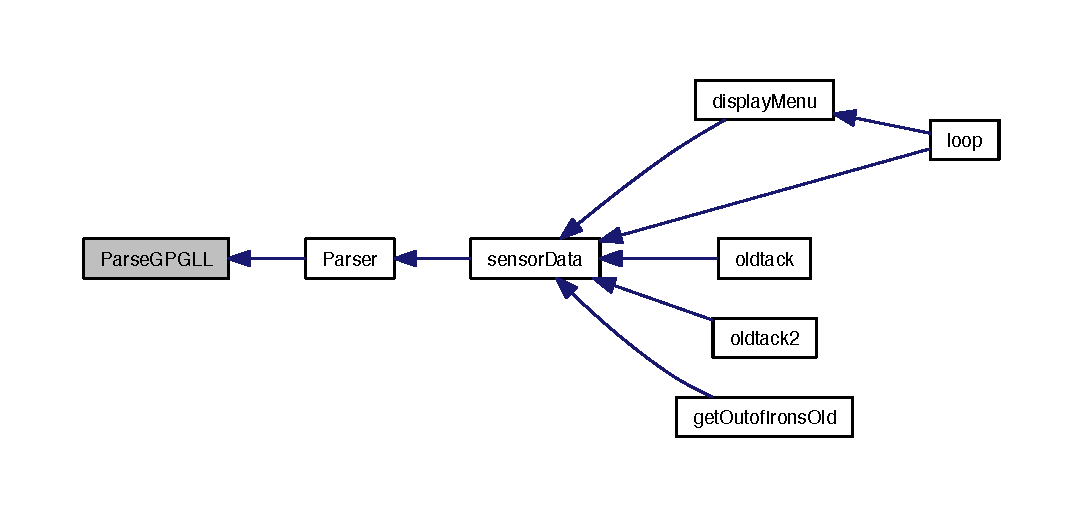
\includegraphics[width=350pt]{_parsing_functions_8pde_a601e25d1a7636238ce5083c54461a17f_icgraph}
\end{center}
\end{figure}


\hypertarget{_parsing_functions_8pde_a9cf045f6db34fd4e2388047fe8045294}{
\index{\-Parsing\-Functions.\-pde@{\-Parsing\-Functions.\-pde}!\-Parser@{\-Parser}}
\index{\-Parser@{\-Parser}!ParsingFunctions.pde@{\-Parsing\-Functions.\-pde}}
\subsubsection[{\-Parser}]{\setlength{\rightskip}{0pt plus 5cm}int \-Parser (
\begin{DoxyParamCaption}
\item[{char $\ast$}]{val}
\end{DoxyParamCaption}
)}}
\label{_parsing_functions_8pde_a9cf045f6db34fd4e2388047fe8045294}


\-Definition at line 64 of file \-Parsing\-Functions.\-pde.



\-Here is the call graph for this function\-:\nopagebreak
\begin{figure}[H]
\begin{center}
\leavevmode
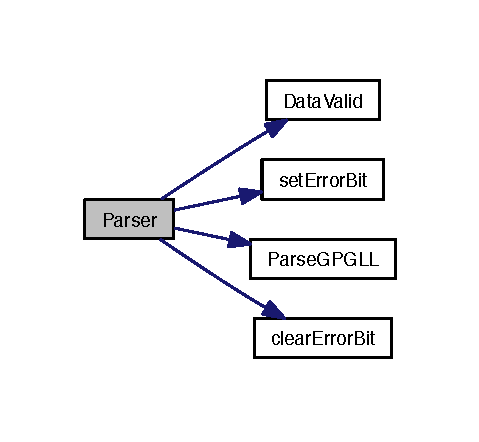
\includegraphics[width=230pt]{_parsing_functions_8pde_a9cf045f6db34fd4e2388047fe8045294_cgraph}
\end{center}
\end{figure}




\-Here is the caller graph for this function\-:\nopagebreak
\begin{figure}[H]
\begin{center}
\leavevmode
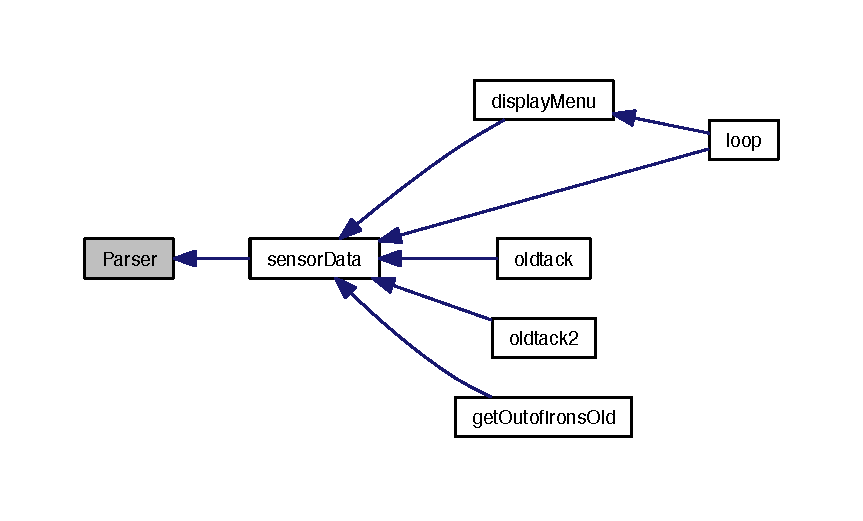
\includegraphics[width=350pt]{_parsing_functions_8pde_a9cf045f6db34fd4e2388047fe8045294_icgraph}
\end{center}
\end{figure}



\hypertarget{sailcode__alpha6_8pde}{
\section{/\-Users/allgood38/\-Desktop/qmast/sailcode\-\_\-alpha6/sailcode\-\_\-alpha6.pde \-File \-Reference}
\label{sailcode__alpha6_8pde}\index{/\-Users/allgood38/\-Desktop/qmast/sailcode\-\_\-alpha6/sailcode\-\_\-alpha6.\-pde@{/\-Users/allgood38/\-Desktop/qmast/sailcode\-\_\-alpha6/sailcode\-\_\-alpha6.\-pde}}
}
{\ttfamily \#include \char`\"{}\-Location\-Struct.\-h\char`\"{}}\*
{\ttfamily \#include $<$\-Software\-Serial.\-h$>$}\*
{\ttfamily \#include $<$stdio.\-h$>$}\*
{\ttfamily \#include $<$avr/io.\-h$>$}\*
\-Include dependency graph for sailcode\-\_\-alpha6.pde\-:\nopagebreak
\begin{figure}[H]
\begin{center}
\leavevmode
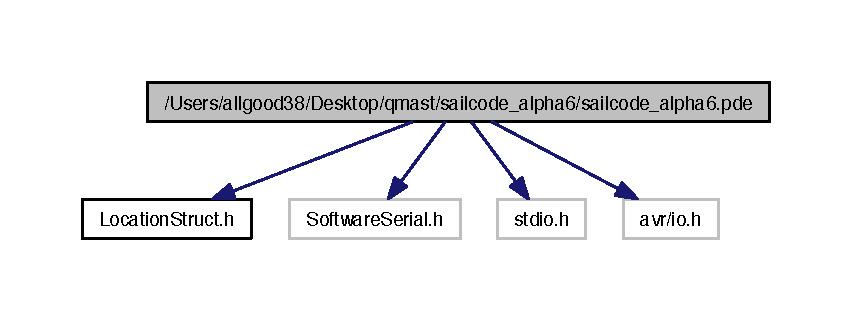
\includegraphics[width=350pt]{sailcode__alpha6_8pde__incl}
\end{center}
\end{figure}
\subsection*{\-Defines}
\begin{DoxyCompactItemize}
\item 
\#define \hyperlink{group__globalconstants_ga2cf0d7fd0783e401cdb0dc31e2179673}{\-T\-A\-C\-K\-I\-N\-G\-\_\-\-A\-N\-G\-L\-E}~40
\begin{DoxyCompactList}\small\item\em \-Boat parameter constants in globalconstants. \end{DoxyCompactList}\item 
\#define \hyperlink{group__globalconstants_ga19af76681fc030672f41555a55f8e8db}{\-M\-A\-R\-K\-\_\-\-D\-I\-S\-T\-A\-N\-C\-E}~4
\begin{DoxyCompactList}\small\item\em \-Course \-Navigation constants. \end{DoxyCompactList}\item 
\#define \hyperlink{group__globalconstants_ga90af33a69f96f733c581db0261bc1676}{\-S\-T\-A\-T\-I\-O\-N\-\_\-\-K\-E\-E\-P\-I\-N\-G\-\_\-\-R\-A\-D\-I\-U\-S}~15
\begin{DoxyCompactList}\small\item\em \-Station keeping navigation constants. \end{DoxyCompactList}\item 
\#define \hyperlink{group__globalconstants_ga0e751f6a929915f9b2ea482bc096d3ca}{\-W\-I\-N\-D\-\_\-\-C\-H\-A\-N\-G\-E\-\_\-\-T\-H\-R\-E\-S\-H\-O\-L\-D}~10
\item 
\#define \hyperlink{group__globalconstants_ga2c1c653e45c4962f05cb6341f359707d}{\-B\-U\-F\-F\-\_\-\-M\-A\-X}~511
\begin{DoxyCompactList}\small\item\em serial data constants \end{DoxyCompactList}\item 
\#define \hyperlink{group__globalconstants_gaa0fe8a3893ebea828d2bb49ef23e3530}{\-D\-E\-G\-R\-E\-E\-\_\-\-T\-O\-\_\-\-M\-I\-N\-U\-T\-E}~60
\begin{DoxyCompactList}\small\item\em \-Calculation constantes. \end{DoxyCompactList}\item 
\#define \hyperlink{group__globalconstants_ga334339ea1bc712a2689665192c02bfad}{\-L\-A\-T\-I\-T\-U\-D\-E\-\_\-\-T\-O\-\_\-\-M\-E\-T\-E\-R}~1855
\begin{DoxyCompactList}\small\item\em \-There are (approximately) 1855 meters in a minute of latitude everywhere; \-This isn't true for longitude, as it depends on the latitude. \end{DoxyCompactList}\item 
\#define \hyperlink{group__globalconstants_ga5944046f3cb8cd99f5f71c1327ef8bc7}{\-L\-O\-N\-G\-I\-T\-U\-D\-E\-\_\-\-T\-O\-\_\-\-M\-E\-T\-E\-R}~1314
\item 
\#define \hyperlink{group__globalconstants_ga1bc4f63dcd0b30d09b7e320d0595695c}{no\-Data\-Bit}~0
\begin{DoxyCompactList}\small\item\em no data, error error bit \end{DoxyCompactList}\item 
\#define \hyperlink{group__globalconstants_gaed67540d9d2621c3a21a0f6eb8b75d01}{old\-Data\-Bit}~1
\begin{DoxyCompactList}\small\item\em there is data, but buffer is full, error bit \end{DoxyCompactList}\item 
\#define \hyperlink{group__globalconstants_gacd110736362ec97d7349dd67b527df39}{checksum\-Bad\-Bit}~2
\begin{DoxyCompactList}\small\item\em indicates checksum fail on data \end{DoxyCompactList}\item 
\#define \hyperlink{group__globalconstants_gae059b25098726f37143284774ef86a07}{two\-Commas\-Bit}~3
\begin{DoxyCompactList}\small\item\em indicates that there were two commas in the data, and it has been discarded and not parsed \end{DoxyCompactList}\item 
\#define \hyperlink{group__globalconstants_ga72f54d1e0beda470c8361ba984148900}{rollover\-Data\-Bit}~4
\begin{DoxyCompactList}\small\item\em \-Indicates data rolled over, not fast enough. \end{DoxyCompactList}\item 
\#define \hyperlink{group__globalconstants_ga69c4923d7bb43a1880f9fbb878bed927}{bad\-Compass\-Data\-Bit}~5
\begin{DoxyCompactList}\small\item\em indicates that strtok did not return \-P\-T\-N\-T\-H\-T\-M, so we probably got bad data \end{DoxyCompactList}\item 
\#define \hyperlink{group__globalconstants_ga808c40e80d82d52b2ceab81282ad35ec}{too\-Much\-Roll\-Bit}~6
\begin{DoxyCompactList}\small\item\em indicates the boat is falling over \end{DoxyCompactList}\item 
\#define \hyperlink{group__globalconstants_ga55cee1ec4df41dd9b7b71c6aa9619bfc}{bad\-Wind\-Data}~7
\begin{DoxyCompactList}\small\item\em indicates an error from the wind sensor \end{DoxyCompactList}\item 
\#define \hyperlink{group__globalconstants_ga5219c41d9ae91432ffb55ec7aeef8873}{bad\-Gps\-Data}~8
\begin{DoxyCompactList}\small\item\em indicates error in gps data \end{DoxyCompactList}\item 
\#define \hyperlink{group__globalconstants_gaaadbf956e6981264e6bf369a08269821}{\-A\-L\-L\-\_\-\-I\-N}~0
\begin{DoxyCompactList}\small\item\em \-Constant which defines when the boat is \char`\"{}\-All In\char`\"{}. \end{DoxyCompactList}\item 
\#define \hyperlink{group__globalconstants_ga074485974be5a03e711020873d83fd90}{\-A\-L\-L\-\_\-\-O\-U\-T}~100
\begin{DoxyCompactList}\small\item\em \-Constant which defines when the boat is \char`\"{}\-All Out\char`\"{}. \end{DoxyCompactList}\item 
\#define \hyperlink{group__globalconstants_gad67ff299260393832da3b34efaaee56a}{reset\-Pin}~8
\begin{DoxyCompactList}\small\item\em \-Pololu reset (digital pin on arduino) \end{DoxyCompactList}\item 
\#define \hyperlink{group__globalconstants_ga38340aff22e726c77f9cf87b5bea10dd}{tx\-Pin}~9
\begin{DoxyCompactList}\small\item\em \-Pololu serial pin (with \-Software\-Serial library) \end{DoxyCompactList}\item 
\#define \hyperlink{group__globalconstants_gac6759acd1da41c55495c6e5ee91e86e9}{\-S\-H\-O\-R\-T\-E\-S\-T\-\_\-\-N\-M\-E\-A}~5
\begin{DoxyCompactList}\small\item\em \-The shortest possible \-N\-M\-E\-A \-String. \end{DoxyCompactList}\item 
\#define \hyperlink{group__globalconstants_ga0038dced6b4ccdfe2ef833cc1965ca73}{\-L\-O\-N\-G\-E\-S\-T\-\_\-\-N\-M\-E\-A}~120
\begin{DoxyCompactList}\small\item\em \-The longest possible \-N\-M\-E\-A \-String. \end{DoxyCompactList}\end{DoxyCompactItemize}
\subsection*{\-Functions}
\begin{DoxyCompactItemize}
\item 
void \hyperlink{sailcode__alpha6_8pde_a4fc01d736fe50cf5b977f755b675f11d}{setup} ()
\item 
void \hyperlink{sailcode__alpha6_8pde_afe461d27b9c48d5921c00d521181f12f}{loop} ()
\end{DoxyCompactItemize}
\subsection*{\-Variables}
\begin{DoxyCompactItemize}
\item 
int \hyperlink{group__group1_gaf9d919ceea98cf74d8ee327ca87871ee}{extra\-Wind\-Data} = 0
\begin{DoxyCompactList}\small\item\em \-Contains extra data from the \-Wind \-Sensor. \end{DoxyCompactList}\item 
int \hyperlink{group__group1_gaafded9aee7842e71393cafc5ac68d921}{extra\-Compass\-Data} = 0
\item 
int \hyperlink{group__group1_gaf7ce3159cdebccf941f8db4e70f5764e}{saved\-Wind\-Checksum} = 0
\begin{DoxyCompactList}\small\item\em clear the global saved \-X\-O\-R value \end{DoxyCompactList}\item 
int \hyperlink{group__group1_gabc070e9e6f6449471852bd233593d1d2}{saved\-Wind\-Xor\-State} = 0
\begin{DoxyCompactList}\small\item\em clear the global saved \-X\-O\-Rstate value \end{DoxyCompactList}\item 
int \hyperlink{group__group1_ga6e28e651127135816788318d7b473dc8}{saved\-Compass\-Checksum} = 0
\item 
int \hyperlink{group__group1_ga766482b676879097212dc7aba1450aa0}{saved\-Compass\-Xor\-State} = 0
\item 
char \hyperlink{group__group1_ga5a0e345949d7a23900298d33d0be150c}{extra\-Wind\-Data\-Array} \mbox{[}\-L\-O\-N\-G\-E\-S\-T\-\_\-\-N\-M\-E\-A\mbox{]}
\begin{DoxyCompactList}\small\item\em a buffer to store roll-\/over data in case this data is fetched mid-\/line \end{DoxyCompactList}\item 
char \hyperlink{group__group1_ga87dbc2b6143e295eae5c571f1b5f460d}{extra\-Compass\-Data\-Array} \mbox{[}\-L\-O\-N\-G\-E\-S\-T\-\_\-\-N\-M\-E\-A\mbox{]}
\item 
float \hyperlink{group__group1_gac5682e48513a771560df50e3b213e61a}{heading}
\begin{DoxyCompactList}\small\item\em heading relative to true north, do not use, only updating 2 times a second \end{DoxyCompactList}\item 
float \hyperlink{group__group1_gad20d9e23979c81b96a060830d0d460a6}{deviation}
\begin{DoxyCompactList}\small\item\em deviation relative to true north; do we use this in our calculations? \-Nope \end{DoxyCompactList}\item 
float \hyperlink{group__group1_gaec967762d2c44e3594070dca470ae334}{variance}
\begin{DoxyCompactList}\small\item\em variance relative to true north; do we use this in our calculations? \-Nope \end{DoxyCompactList}\item 
float \hyperlink{group__group1_ga3c5844d05a57a968ed5686a10e4a5af8}{bspeed}
\begin{DoxyCompactList}\small\item\em \-Boat's speed in km/h. \end{DoxyCompactList}\item 
float \hyperlink{group__group1_ga6ebc5b99dfacc747433709383f3bea8c}{bspeedk}
\begin{DoxyCompactList}\small\item\em \-Boat's speed in knots. \end{DoxyCompactList}\item 
float \hyperlink{group__group1_ga6bc5259b7cc1cb6128495b28f55b0a5d}{wind\-\_\-angl}
\begin{DoxyCompactList}\small\item\em wind angle, (relative to boat \-I believe, could be north, check this) \end{DoxyCompactList}\item 
float \hyperlink{group__group1_ga641fd5e4834deb5465b1931b7645457d}{wind\-\_\-velocity}
\begin{DoxyCompactList}\small\item\em wind velocity in knots \end{DoxyCompactList}\item 
float \hyperlink{group__group1_ga4736792191ccbbbb7b3d6933a3302336}{headingc}
\begin{DoxyCompactList}\small\item\em \-Heading from compass. \end{DoxyCompactList}\item 
float \hyperlink{group__group1_ga282e7d4378d4a18a805b8980295ac86c}{pitch}
\begin{DoxyCompactList}\small\item\em pitch \end{DoxyCompactList}\item 
float \hyperlink{group__group1_ga26fd84d522945b6038221d9e38c7cc39}{roll}
\begin{DoxyCompactList}\small\item\em roll \end{DoxyCompactList}\item 
float \hyperlink{group__group1_gaea221e98c9a7c4e63325dc52ab83c14d}{true\-Wind}
\begin{DoxyCompactList}\small\item\em wind direction calculated at checkteck \end{DoxyCompactList}\item 
int \hyperlink{group__group1_ga8b212bdc5d94214c0e3803a696f2f676}{rudder\-Val}
\item 
int \hyperlink{group__group1_ga1fee0a7eb4ae243dcc5afe20f508990e}{jib\-Val}
\item 
int \hyperlink{group__group1_ga3c5dac52b53dc3642a843a7d6a9266ca}{main\-Val}
\item 
float \hyperlink{group__group1_ga8d6cfa64e358c393d2d13c5a9803e052}{heading\-Val}
\begin{DoxyCompactList}\small\item\em where we are going, temporary compass smoothing test \end{DoxyCompactList}\item 
float \hyperlink{group__group1_ga90176c4024ce3ce161b5feda285f97c5}{distance\-Val}
\begin{DoxyCompactList}\small\item\em distance to next waypoint one-\/shots, no averaging, present conditions \end{DoxyCompactList}\item 
float \hyperlink{group__group1_ga3c596663ba52aec96df1f504772914be}{heading\-\_\-newest}
\begin{DoxyCompactList}\small\item\em heading relative to true north \end{DoxyCompactList}\item 
float \hyperlink{group__group1_ga9fcee93bab7f0c81f67b99f8b8597e9c}{wind\-\_\-angl\-\_\-newest}
\begin{DoxyCompactList}\small\item\em wind angle, (relative to boat) \end{DoxyCompactList}\item 
\-Software\-Serial \hyperlink{group__group1_gad08dcd7d87414b8d7f7e9cf2689ea5d8}{servo\-\_\-ser} = \-Software\-Serial(7, tx\-Pin)
\item 
int \hyperlink{group__group1_gaf79de3204853b3b4101113683e74cd54}{rudder\-Dir} = -\/1
\begin{DoxyCompactList}\small\item\em global for reversing rudder if we are parking lot testing \end{DoxyCompactList}\item 
int \hyperlink{group__group1_gaf7f8f4a4e39e09fdb5e9f02330ecabef}{points}
\begin{DoxyCompactList}\small\item\em max waypoints selected for travel \end{DoxyCompactList}\item 
int \hyperlink{group__group1_ga2dee8b7fcecc7c2d190e9304b43ea886}{point}
\begin{DoxyCompactList}\small\item\em point for sail to waypoint in menu \end{DoxyCompactList}\item 
int \hyperlink{group__group1_ga9c43dea25777e23791d530b06f6715f1}{current\-Point} = 0
\begin{DoxyCompactList}\small\item\em current waypoint on course of travel \end{DoxyCompactList}\item 
int \hyperlink{group__group1_gac9d865c1411ae815f6b2394c45d604e7}{\-Straight\-Sail\-Direction}
\item 
int \hyperlink{group__group1_ga79863a7d6b31d0c89c5050c2cd931cfe}{\-Current\-Selection}
\item 
long \hyperlink{group__group1_ga8ad49a66e91d8658c5f1f7dbcbcbbd2f}{start\-Time}
\item 
int \hyperlink{group__group1_gaffc96d075c8796c3d5ef3dc5824c0819}{station\-Counter}
\item 
boolean \hyperlink{group__group1_gaf453f5fa6c0df67707ca308a2fc80ca1}{times\-Up}
\item 
int \hyperlink{group__group1_gabe157ddfb46568e2de8b041f54ac6d98}{\-Station\-Keeping\-Time\-In\-Box} = 270000
\item 
boolean \hyperlink{group__group1_gab23a7a79ede8d141fa92f4475d36fb24}{tacking}
\item 
int \hyperlink{group__group1_gabdfa4a25e22806c47eebd4c9826ef7a6}{tacking\-Side}
\item 
int \hyperlink{group__group1_ga332365589e9af9d8ec4d1c5663034132}{iron\-Time}
\item 
int \hyperlink{group__group1_gab675a39a0c7f0587be9ae6734db7ac80}{error\-Code}
\end{DoxyCompactItemize}


\subsection{\-Function \-Documentation}
\hypertarget{sailcode__alpha6_8pde_afe461d27b9c48d5921c00d521181f12f}{
\index{sailcode\-\_\-alpha6.\-pde@{sailcode\-\_\-alpha6.\-pde}!loop@{loop}}
\index{loop@{loop}!sailcode_alpha6.pde@{sailcode\-\_\-alpha6.\-pde}}
\subsubsection[{loop}]{\setlength{\rightskip}{0pt plus 5cm}void loop (
\begin{DoxyParamCaption}
{}
\end{DoxyParamCaption}
)}}
\label{sailcode__alpha6_8pde_afe461d27b9c48d5921c00d521181f12f}
if menu returned 0, any updating happened in the menu function itself and we want the code to just keep doing what it was doing before (e.\-g. setting \-R\-C mode)

\-Straight \-Sail towards \-N,\-S,\-E,\-W as 0, 180, 90, 270. \-No sail control.

\-Straightsail can no longer be called in isolation, needs sailto\-Waypoint which keeps track of when tacking is necessary

stationskeeps around a single spot in the middle of the square 

\-Definition at line 263 of file sailcode\-\_\-alpha6.\-pde.



\-Here is the call graph for this function\-:\nopagebreak
\begin{figure}[H]
\begin{center}
\leavevmode
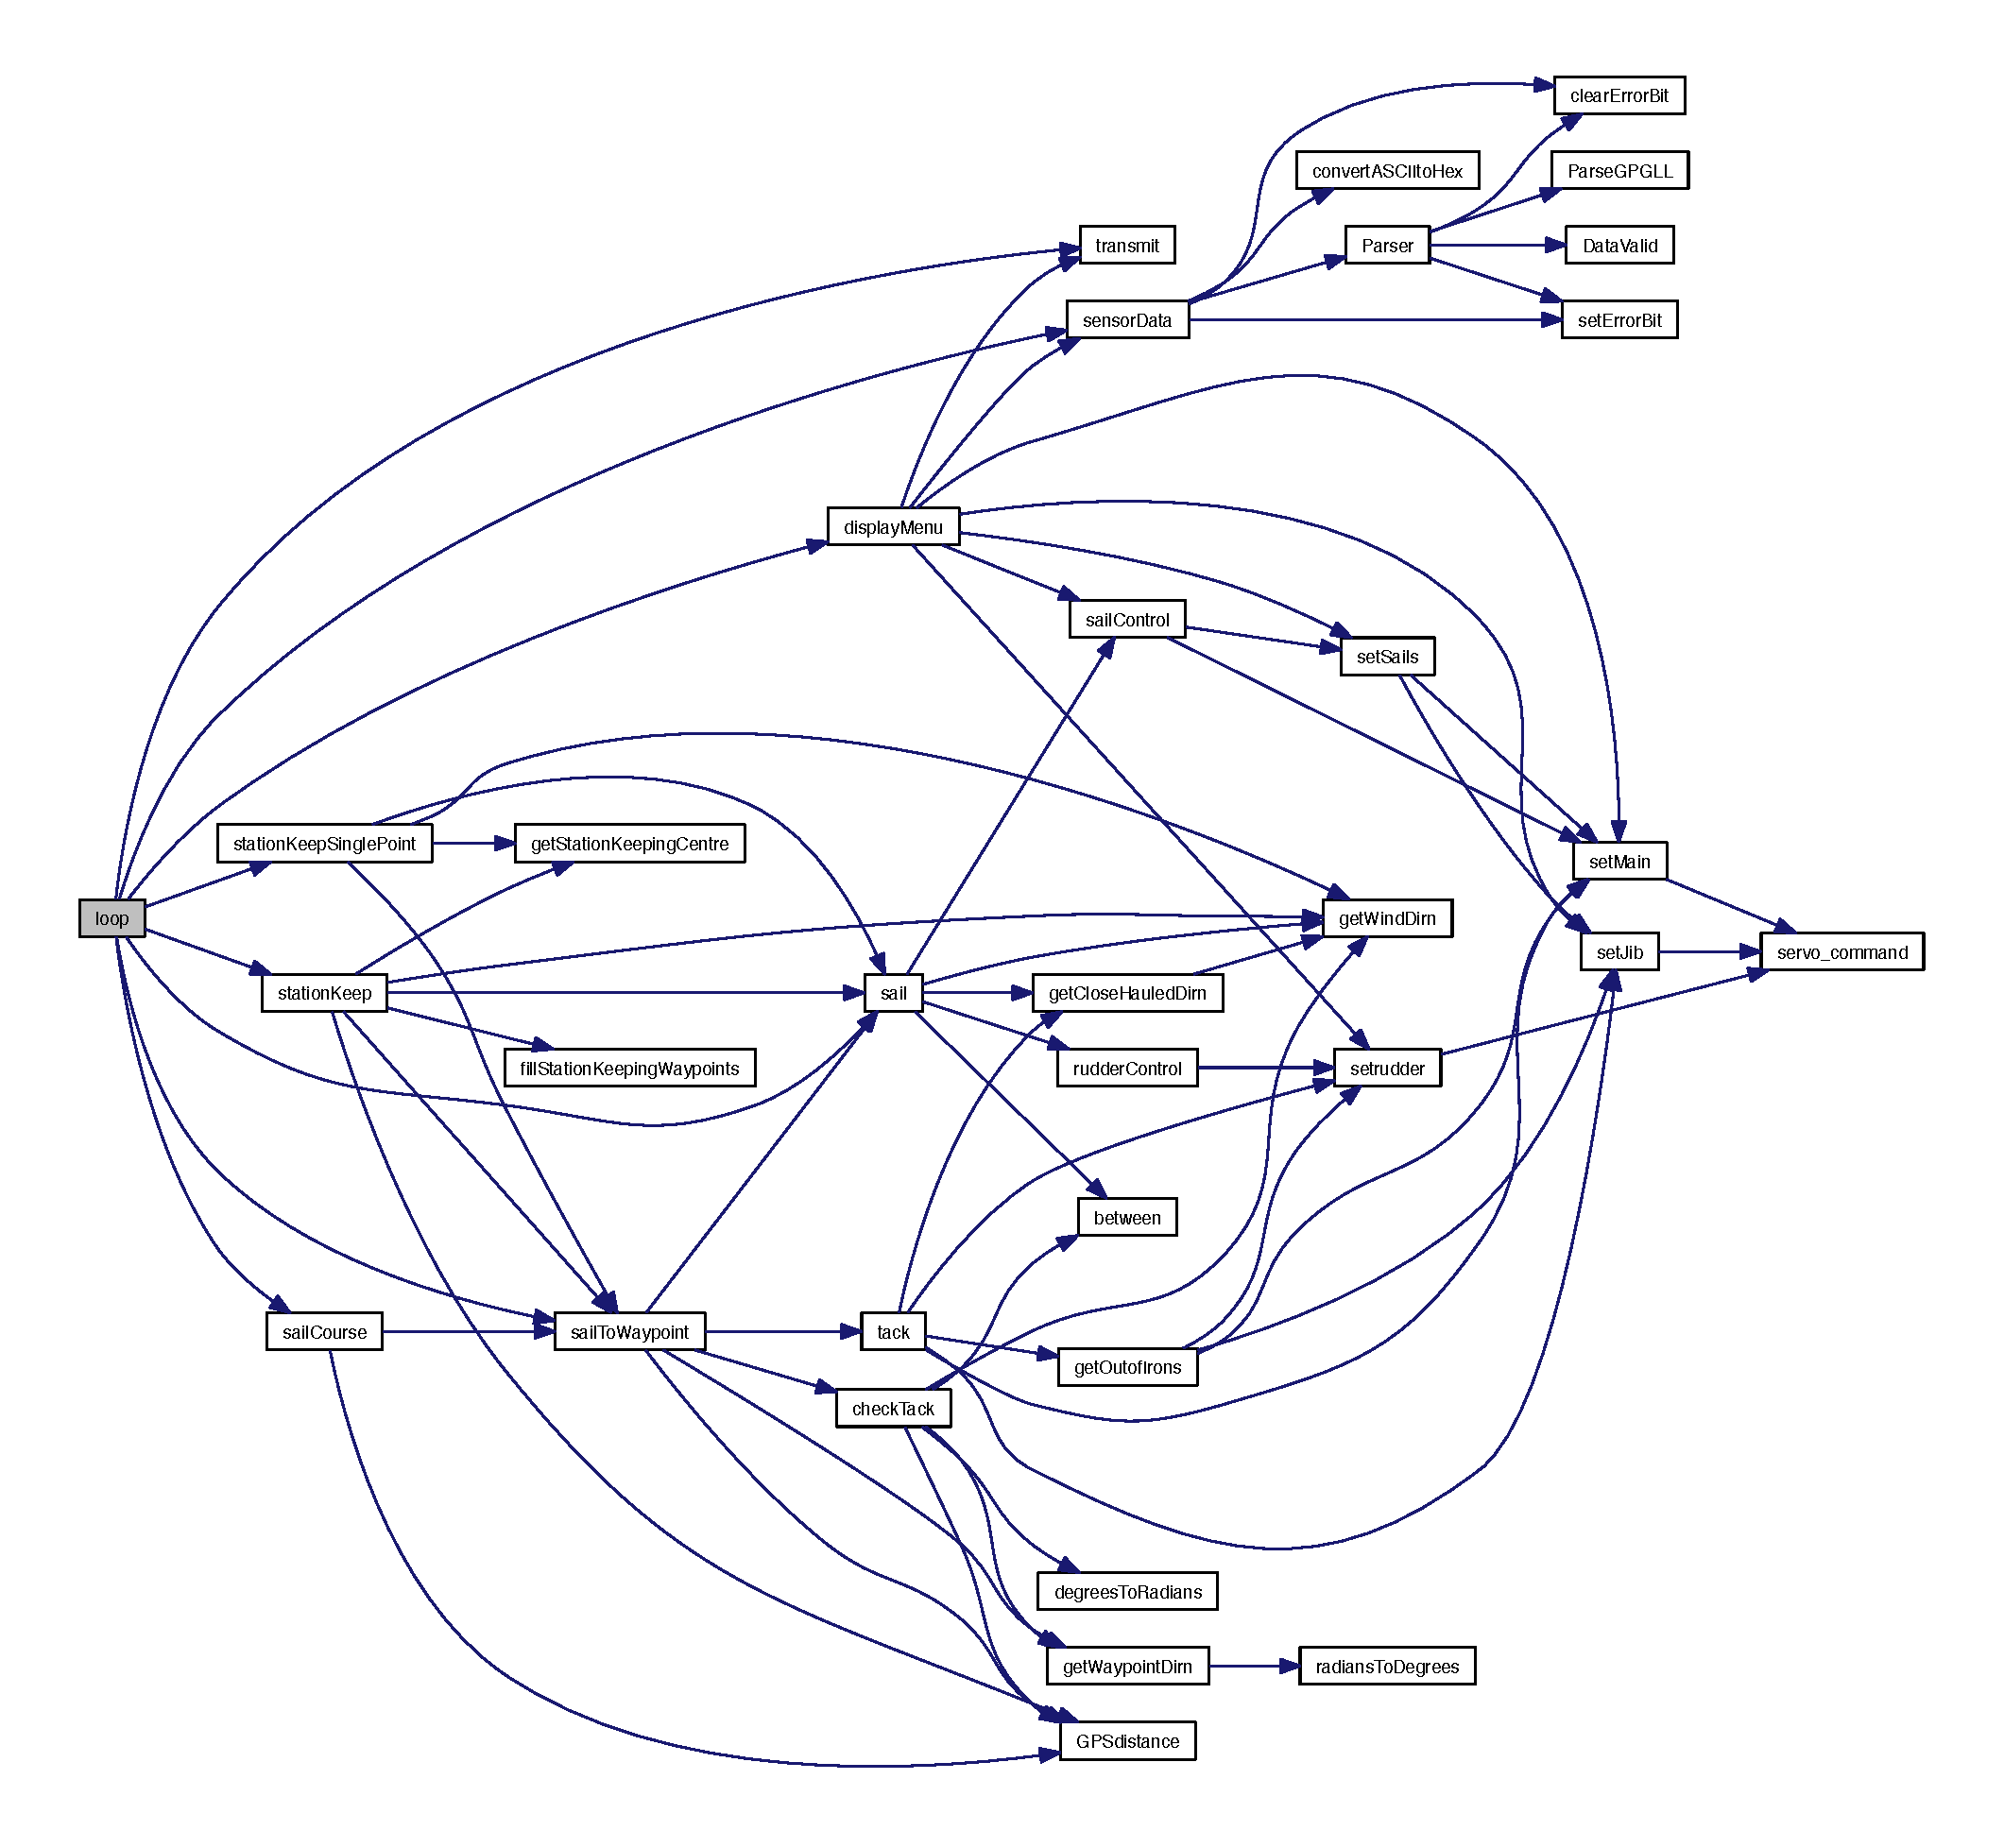
\includegraphics[width=350pt]{sailcode__alpha6_8pde_afe461d27b9c48d5921c00d521181f12f_cgraph}
\end{center}
\end{figure}


\hypertarget{sailcode__alpha6_8pde_a4fc01d736fe50cf5b977f755b675f11d}{
\index{sailcode\-\_\-alpha6.\-pde@{sailcode\-\_\-alpha6.\-pde}!setup@{setup}}
\index{setup@{setup}!sailcode_alpha6.pde@{sailcode\-\_\-alpha6.\-pde}}
\subsubsection[{setup}]{\setlength{\rightskip}{0pt plus 5cm}void setup (
\begin{DoxyParamCaption}
{}
\end{DoxyParamCaption}
)}}
\label{sailcode__alpha6_8pde_a4fc01d736fe50cf5b977f755b675f11d}
\-Change wind to send 5 times a second default for now, need to make sure we can get everything out of the buffer

\-Definition at line 202 of file sailcode\-\_\-alpha6.\-pde.



\-Here is the call graph for this function\-:\nopagebreak
\begin{figure}[H]
\begin{center}
\leavevmode
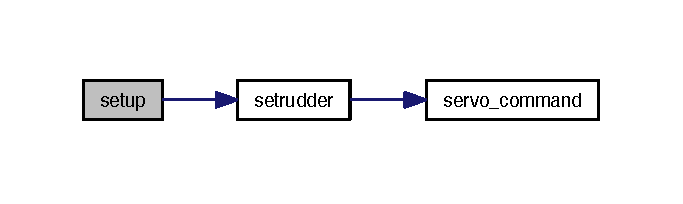
\includegraphics[width=328pt]{sailcode__alpha6_8pde_a4fc01d736fe50cf5b977f755b675f11d_cgraph}
\end{center}
\end{figure}



\hypertarget{_sailing_logic_8pde}{
\section{/\-Users/allgood38/\-Desktop/qmast/sailcode\-\_\-alpha6/\-Sailing\-Logic.pde \-File \-Reference}
\label{_sailing_logic_8pde}\index{/\-Users/allgood38/\-Desktop/qmast/sailcode\-\_\-alpha6/\-Sailing\-Logic.\-pde@{/\-Users/allgood38/\-Desktop/qmast/sailcode\-\_\-alpha6/\-Sailing\-Logic.\-pde}}
}
\subsection*{\-Functions}
\begin{DoxyCompactItemize}
\item 
void \hyperlink{_sailing_logic_8pde_aeaba10e3002bd9b9fd2ea1bdd5ab97ea}{sail\-Course} ()
\begin{DoxyCompactList}\small\item\em \-Alternate sailcourse code by laz. \end{DoxyCompactList}\item 
void \hyperlink{_sailing_logic_8pde_a42829044eaaf781783f525dbf35eabc1}{sail\-To\-Waypoint} (struct \hyperlink{structpoints}{points} waypoint)
\begin{DoxyCompactList}\small\item\em \-Checks to see if the boat should sail or tack, thats it. \end{DoxyCompactList}\item 
void \hyperlink{_sailing_logic_8pde_a8e7082b5e8ca95936e2afa33af9f6835}{sail} (int waypoint\-Dirn)
\begin{DoxyCompactList}\small\item\em \-Sails towards the waypoint\-Dirn passed, in which case it sails closehauled. \end{DoxyCompactList}\item 
boolean \hyperlink{_sailing_logic_8pde_a1acad42611d693fa074f7dae5e5a5e3f}{check\-Tack} (int corridor\-Half\-Width, struct \hyperlink{structpoints}{points} waypoint)
\begin{DoxyCompactList}\small\item\em \-Check to see if tacking is necessary. \end{DoxyCompactList}\item 
void \hyperlink{_sailing_logic_8pde_aae8de392da41d229212d9943d965690c}{sail\-Control} ()
\begin{DoxyCompactList}\small\item\em \-This function controls the sails, proportional to the wind direction with no consideration for wind strength. \end{DoxyCompactList}\item 
int \hyperlink{_sailing_logic_8pde_aad7e4cc1e18478540e9c1d8c00390d24}{rudder\-Control} (int direction\-Error)
\begin{DoxyCompactList}\small\item\em \-Controls the rudder movement, used to be part of sail. \end{DoxyCompactList}\end{DoxyCompactItemize}


\subsection{\-Function \-Documentation}
\hypertarget{_sailing_logic_8pde_a1acad42611d693fa074f7dae5e5a5e3f}{
\index{\-Sailing\-Logic.\-pde@{\-Sailing\-Logic.\-pde}!check\-Tack@{check\-Tack}}
\index{check\-Tack@{check\-Tack}!SailingLogic.pde@{\-Sailing\-Logic.\-pde}}
\subsubsection[{check\-Tack}]{\setlength{\rightskip}{0pt plus 5cm}boolean check\-Tack (
\begin{DoxyParamCaption}
\item[{int}]{corridor\-Half\-Width, }
\item[{struct {\bf points}}]{waypoint}
\end{DoxyParamCaption}
)}}
\label{_sailing_logic_8pde_a1acad42611d693fa074f7dae5e5a5e3f}


\-Check to see if tacking is necessary. 

\-Looks to see if the boat is in the downwind corridor and if its angle to the wind is close-\/hauled then it will tack. \-This results in better turning and will allow for the safety of get\-Out\-Of\-Irons being called during any turn into the wind.


\begin{DoxyParams}[1]{\-Parameters}
\mbox{\tt in}  & {\em corridor\-Half\-Width} & \-Not sure what this is yet \\
\hline
\mbox{\tt in}  & {\em points} & \-Something to do with a waypoint? \\
\hline
\end{DoxyParams}


\-Definition at line 92 of file \-Sailing\-Logic.\-pde.



\-Here is the call graph for this function\-:\nopagebreak
\begin{figure}[H]
\begin{center}
\leavevmode
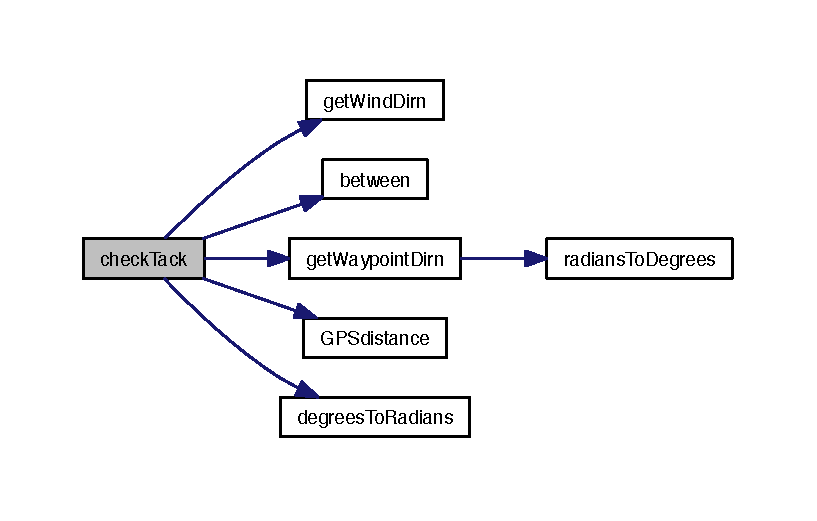
\includegraphics[width=350pt]{_sailing_logic_8pde_a1acad42611d693fa074f7dae5e5a5e3f_cgraph}
\end{center}
\end{figure}




\-Here is the caller graph for this function\-:\nopagebreak
\begin{figure}[H]
\begin{center}
\leavevmode
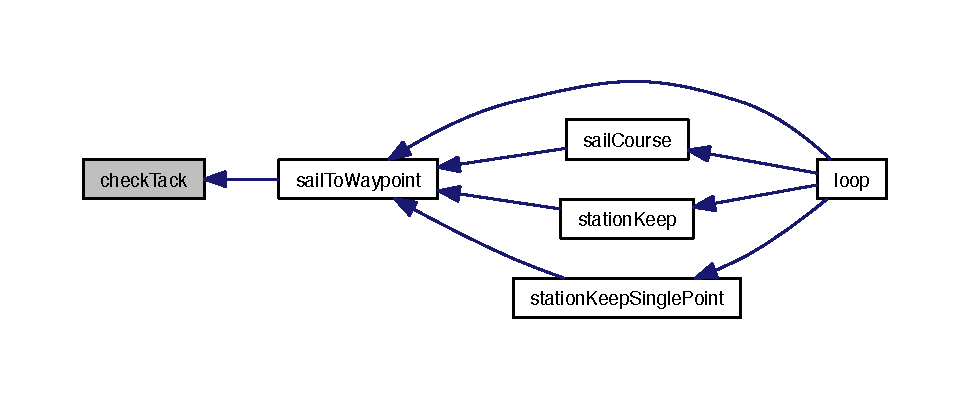
\includegraphics[width=350pt]{_sailing_logic_8pde_a1acad42611d693fa074f7dae5e5a5e3f_icgraph}
\end{center}
\end{figure}


\hypertarget{_sailing_logic_8pde_aad7e4cc1e18478540e9c1d8c00390d24}{
\index{\-Sailing\-Logic.\-pde@{\-Sailing\-Logic.\-pde}!rudder\-Control@{rudder\-Control}}
\index{rudder\-Control@{rudder\-Control}!SailingLogic.pde@{\-Sailing\-Logic.\-pde}}
\subsubsection[{rudder\-Control}]{\setlength{\rightskip}{0pt plus 5cm}int rudder\-Control (
\begin{DoxyParamCaption}
\item[{int}]{direction\-Error}
\end{DoxyParamCaption}
)}}
\label{_sailing_logic_8pde_aad7e4cc1e18478540e9c1d8c00390d24}


\-Controls the rudder movement, used to be part of sail. 

but is moved to a seperate function so it is easier to modify


\begin{DoxyParams}[1]{\-Parameters}
\mbox{\tt in}  & {\em direction\-Error} & \-This needs explanation. \\
\hline
\end{DoxyParams}


\-Definition at line 165 of file \-Sailing\-Logic.\-pde.



\-Here is the call graph for this function\-:\nopagebreak
\begin{figure}[H]
\begin{center}
\leavevmode
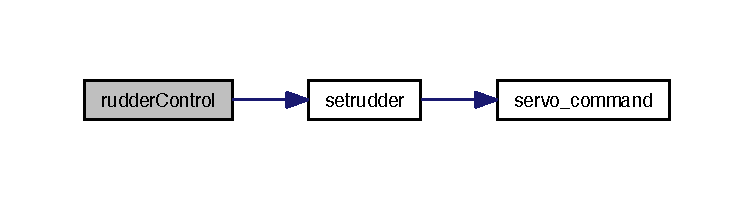
\includegraphics[width=350pt]{_sailing_logic_8pde_aad7e4cc1e18478540e9c1d8c00390d24_cgraph}
\end{center}
\end{figure}




\-Here is the caller graph for this function\-:\nopagebreak
\begin{figure}[H]
\begin{center}
\leavevmode
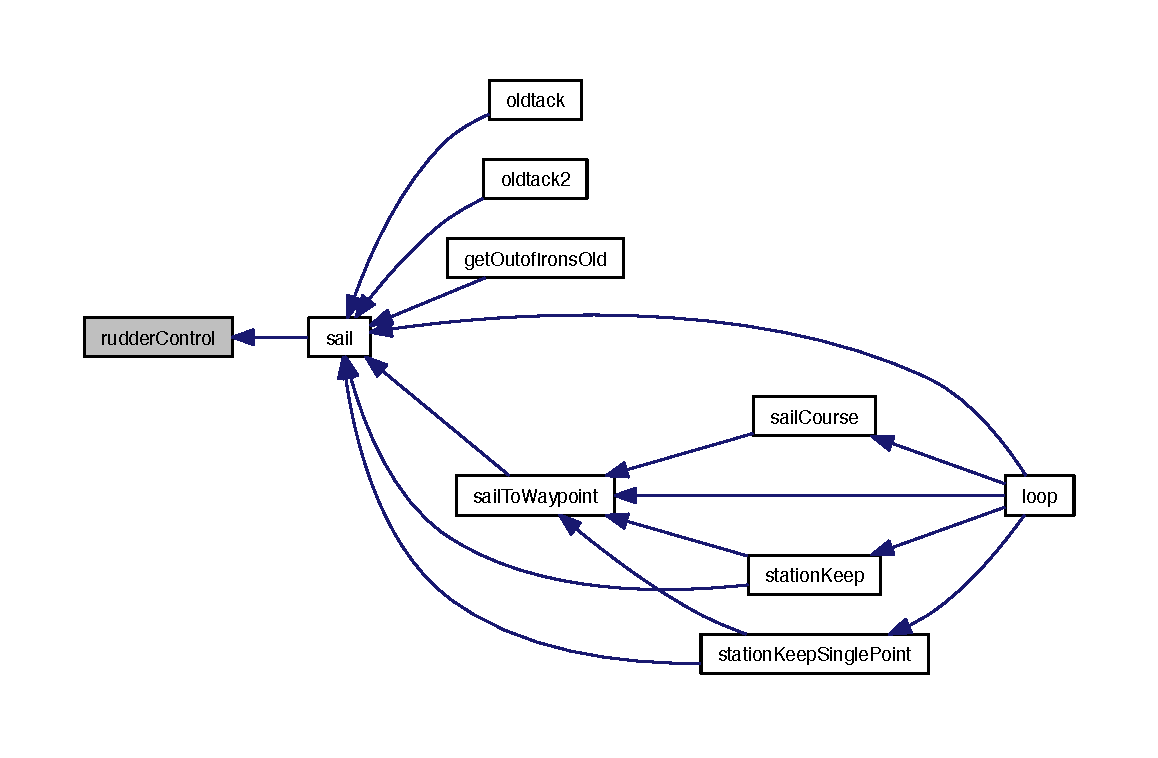
\includegraphics[width=350pt]{_sailing_logic_8pde_aad7e4cc1e18478540e9c1d8c00390d24_icgraph}
\end{center}
\end{figure}


\hypertarget{_sailing_logic_8pde_a8e7082b5e8ca95936e2afa33af9f6835}{
\index{\-Sailing\-Logic.\-pde@{\-Sailing\-Logic.\-pde}!sail@{sail}}
\index{sail@{sail}!SailingLogic.pde@{\-Sailing\-Logic.\-pde}}
\subsubsection[{sail}]{\setlength{\rightskip}{0pt plus 5cm}void sail (
\begin{DoxyParamCaption}
\item[{int}]{waypoint\-Dirn}
\end{DoxyParamCaption}
)}}
\label{_sailing_logic_8pde_a8e7082b5e8ca95936e2afa33af9f6835}


\-Sails towards the waypoint\-Dirn passed, in which case it sails closehauled. 

\-The other funtcion sail\-To\-Waypoint will take care of when tacking is necessary \-This function replaces straightsail which originally only controlled the rudder 

\-Definition at line 63 of file \-Sailing\-Logic.\-pde.



\-Here is the call graph for this function\-:\nopagebreak
\begin{figure}[H]
\begin{center}
\leavevmode
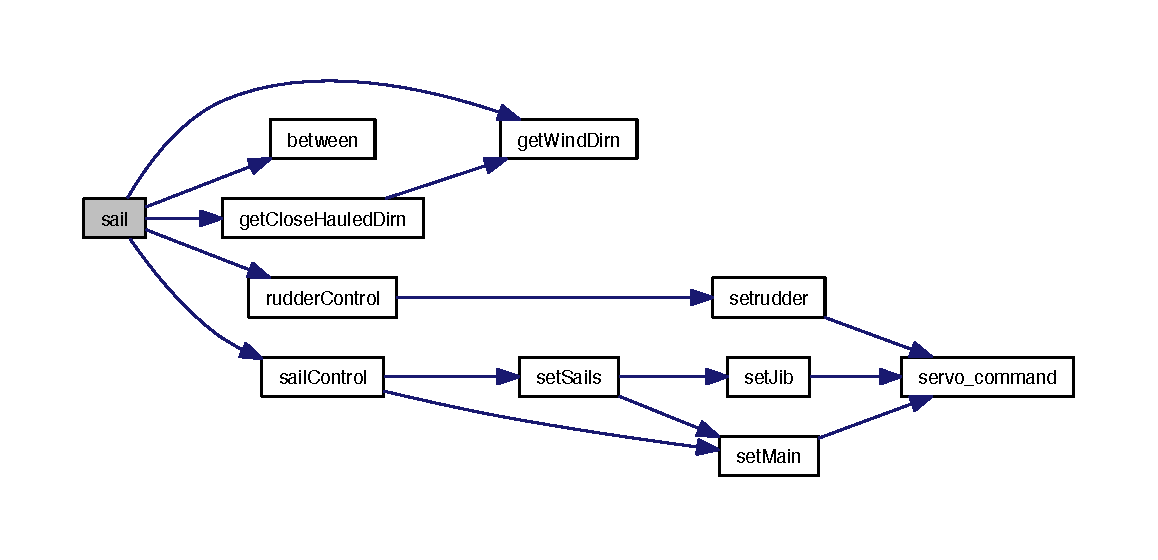
\includegraphics[width=350pt]{_sailing_logic_8pde_a8e7082b5e8ca95936e2afa33af9f6835_cgraph}
\end{center}
\end{figure}




\-Here is the caller graph for this function\-:\nopagebreak
\begin{figure}[H]
\begin{center}
\leavevmode
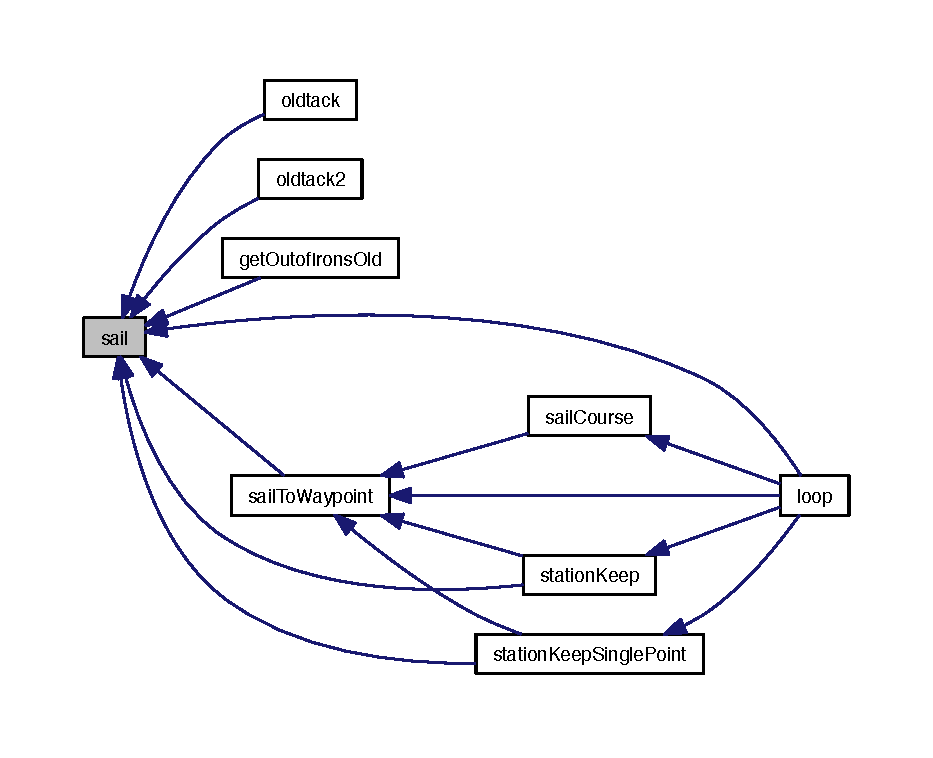
\includegraphics[width=350pt]{_sailing_logic_8pde_a8e7082b5e8ca95936e2afa33af9f6835_icgraph}
\end{center}
\end{figure}


\hypertarget{_sailing_logic_8pde_aae8de392da41d229212d9943d965690c}{
\index{\-Sailing\-Logic.\-pde@{\-Sailing\-Logic.\-pde}!sail\-Control@{sail\-Control}}
\index{sail\-Control@{sail\-Control}!SailingLogic.pde@{\-Sailing\-Logic.\-pde}}
\subsubsection[{sail\-Control}]{\setlength{\rightskip}{0pt plus 5cm}void sail\-Control (
\begin{DoxyParamCaption}
{}
\end{DoxyParamCaption}
)}}
\label{_sailing_logic_8pde_aae8de392da41d229212d9943d965690c}


\-This function controls the sails, proportional to the wind direction with no consideration for wind strength. 



\-Definition at line 136 of file \-Sailing\-Logic.\-pde.



\-Here is the call graph for this function\-:\nopagebreak
\begin{figure}[H]
\begin{center}
\leavevmode
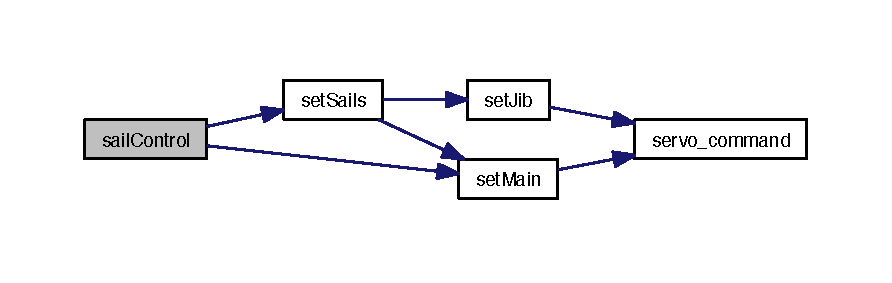
\includegraphics[width=350pt]{_sailing_logic_8pde_aae8de392da41d229212d9943d965690c_cgraph}
\end{center}
\end{figure}




\-Here is the caller graph for this function\-:\nopagebreak
\begin{figure}[H]
\begin{center}
\leavevmode
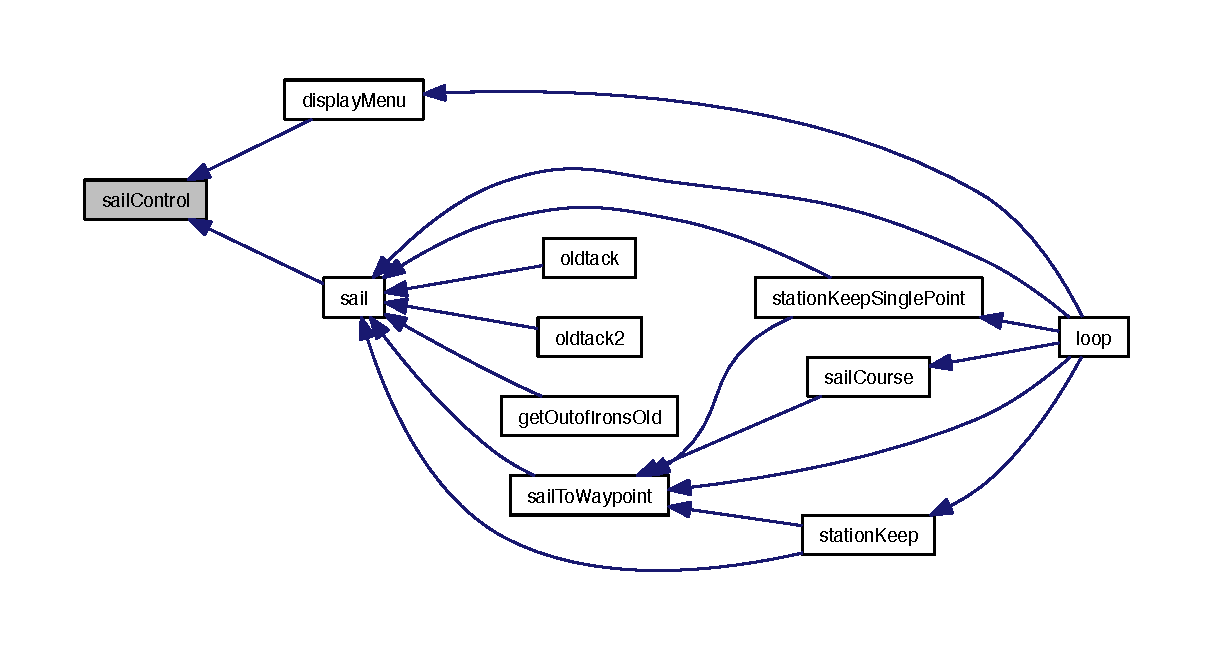
\includegraphics[width=350pt]{_sailing_logic_8pde_aae8de392da41d229212d9943d965690c_icgraph}
\end{center}
\end{figure}


\hypertarget{_sailing_logic_8pde_aeaba10e3002bd9b9fd2ea1bdd5ab97ea}{
\index{\-Sailing\-Logic.\-pde@{\-Sailing\-Logic.\-pde}!sail\-Course@{sail\-Course}}
\index{sail\-Course@{sail\-Course}!SailingLogic.pde@{\-Sailing\-Logic.\-pde}}
\subsubsection[{sail\-Course}]{\setlength{\rightskip}{0pt plus 5cm}void sail\-Course (
\begin{DoxyParamCaption}
{}
\end{DoxyParamCaption}
)}}
\label{_sailing_logic_8pde_aeaba10e3002bd9b9fd2ea1bdd5ab97ea}


\-Alternate sailcourse code by laz. 

\-Works the same but does not use long loops for waypoint selection, less responsive but allows for menu usage while sailing. \-Instead of looping globals keep track of current waypoint, code updates that waypoint when reached and sets boat in the direction of the next one, this will be slightly less responsive as the time between each adjustment will include checking the menu but it should still be fast enough. \-Needs to be tested and compared to existing sailcourse function. \-Original in sailcode5 \-Sail the race course. \-Declare things static so that they persist after each call, eliminate globals $<$ the boat's distance to the present waypoint 

\-Definition at line 17 of file \-Sailing\-Logic.\-pde.



\-Here is the call graph for this function\-:\nopagebreak
\begin{figure}[H]
\begin{center}
\leavevmode
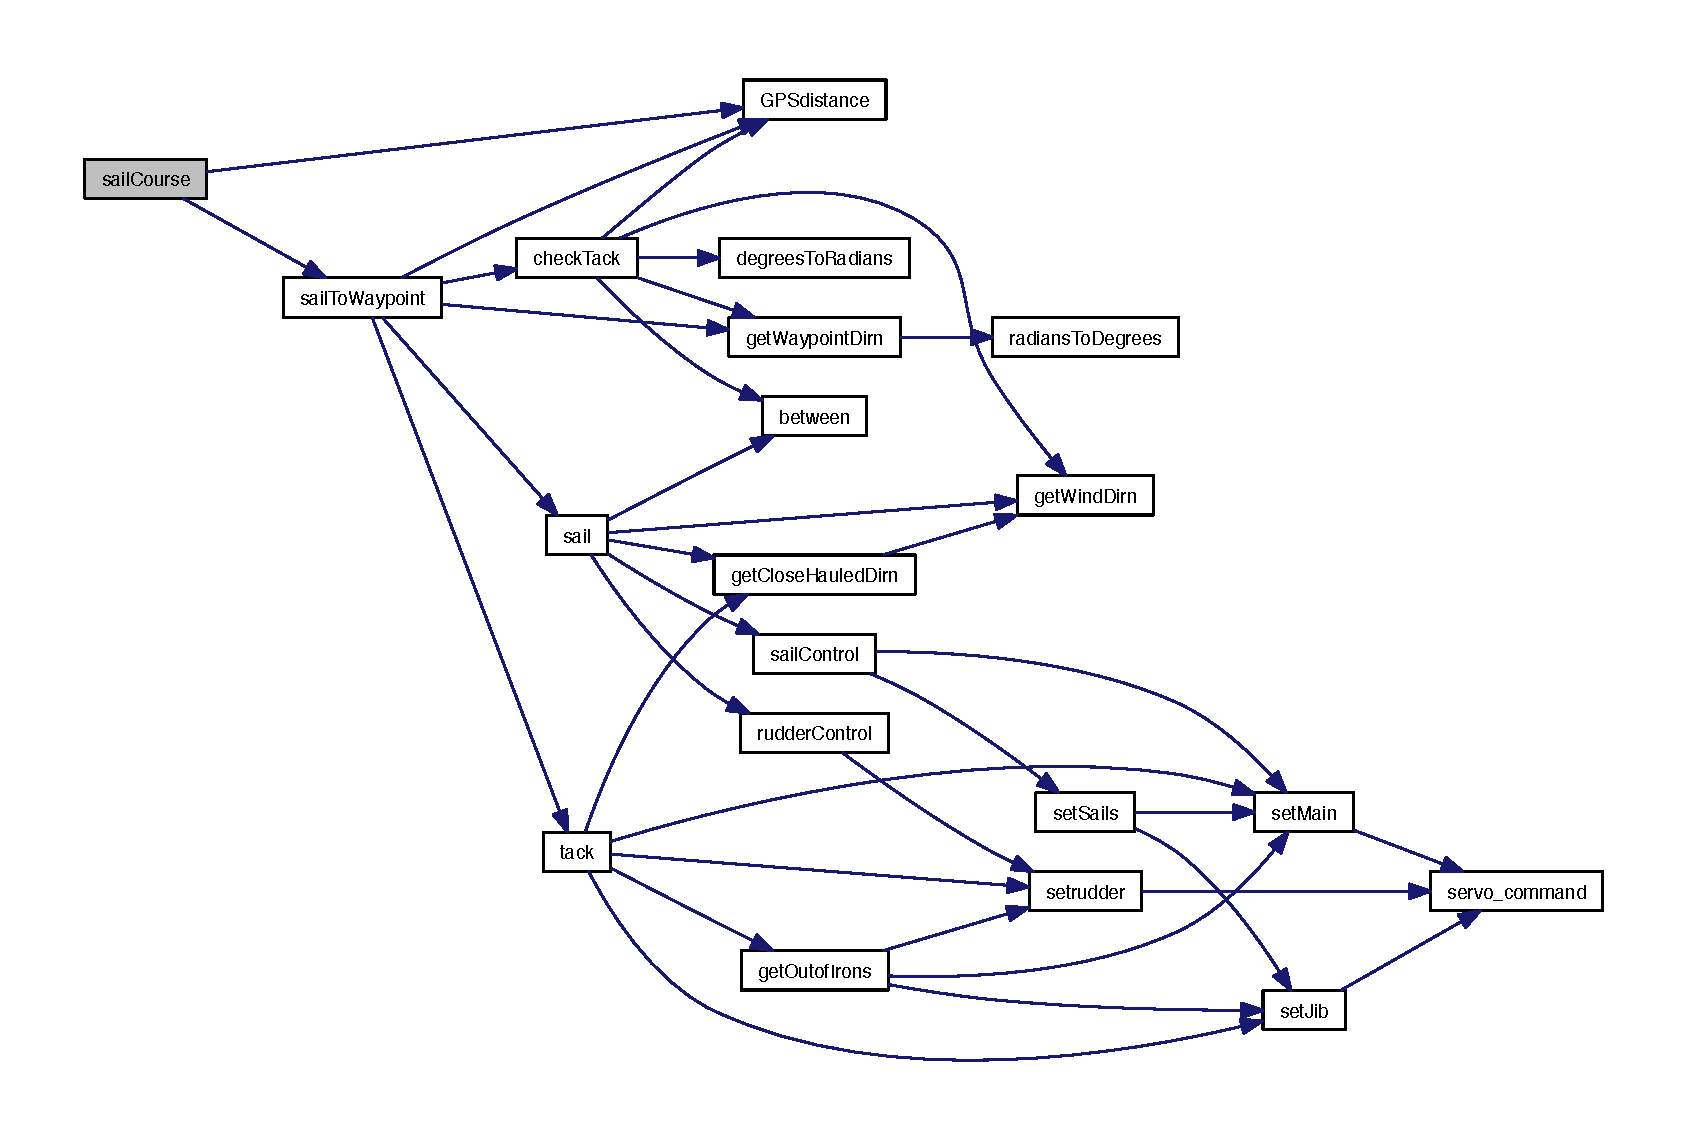
\includegraphics[width=350pt]{_sailing_logic_8pde_aeaba10e3002bd9b9fd2ea1bdd5ab97ea_cgraph}
\end{center}
\end{figure}




\-Here is the caller graph for this function\-:\nopagebreak
\begin{figure}[H]
\begin{center}
\leavevmode
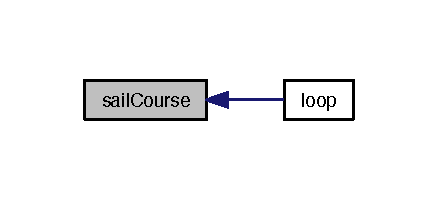
\includegraphics[width=210pt]{_sailing_logic_8pde_aeaba10e3002bd9b9fd2ea1bdd5ab97ea_icgraph}
\end{center}
\end{figure}


\hypertarget{_sailing_logic_8pde_a42829044eaaf781783f525dbf35eabc1}{
\index{\-Sailing\-Logic.\-pde@{\-Sailing\-Logic.\-pde}!sail\-To\-Waypoint@{sail\-To\-Waypoint}}
\index{sail\-To\-Waypoint@{sail\-To\-Waypoint}!SailingLogic.pde@{\-Sailing\-Logic.\-pde}}
\subsubsection[{sail\-To\-Waypoint}]{\setlength{\rightskip}{0pt plus 5cm}void sail\-To\-Waypoint (
\begin{DoxyParamCaption}
\item[{struct {\bf points}}]{waypoint}
\end{DoxyParamCaption}
)}}
\label{_sailing_logic_8pde_a42829044eaaf781783f525dbf35eabc1}


\-Checks to see if the boat should sail or tack, thats it. 

\-This is a newer version of the original function with the same name. 

\-Definition at line 37 of file \-Sailing\-Logic.\-pde.



\-Here is the call graph for this function\-:\nopagebreak
\begin{figure}[H]
\begin{center}
\leavevmode
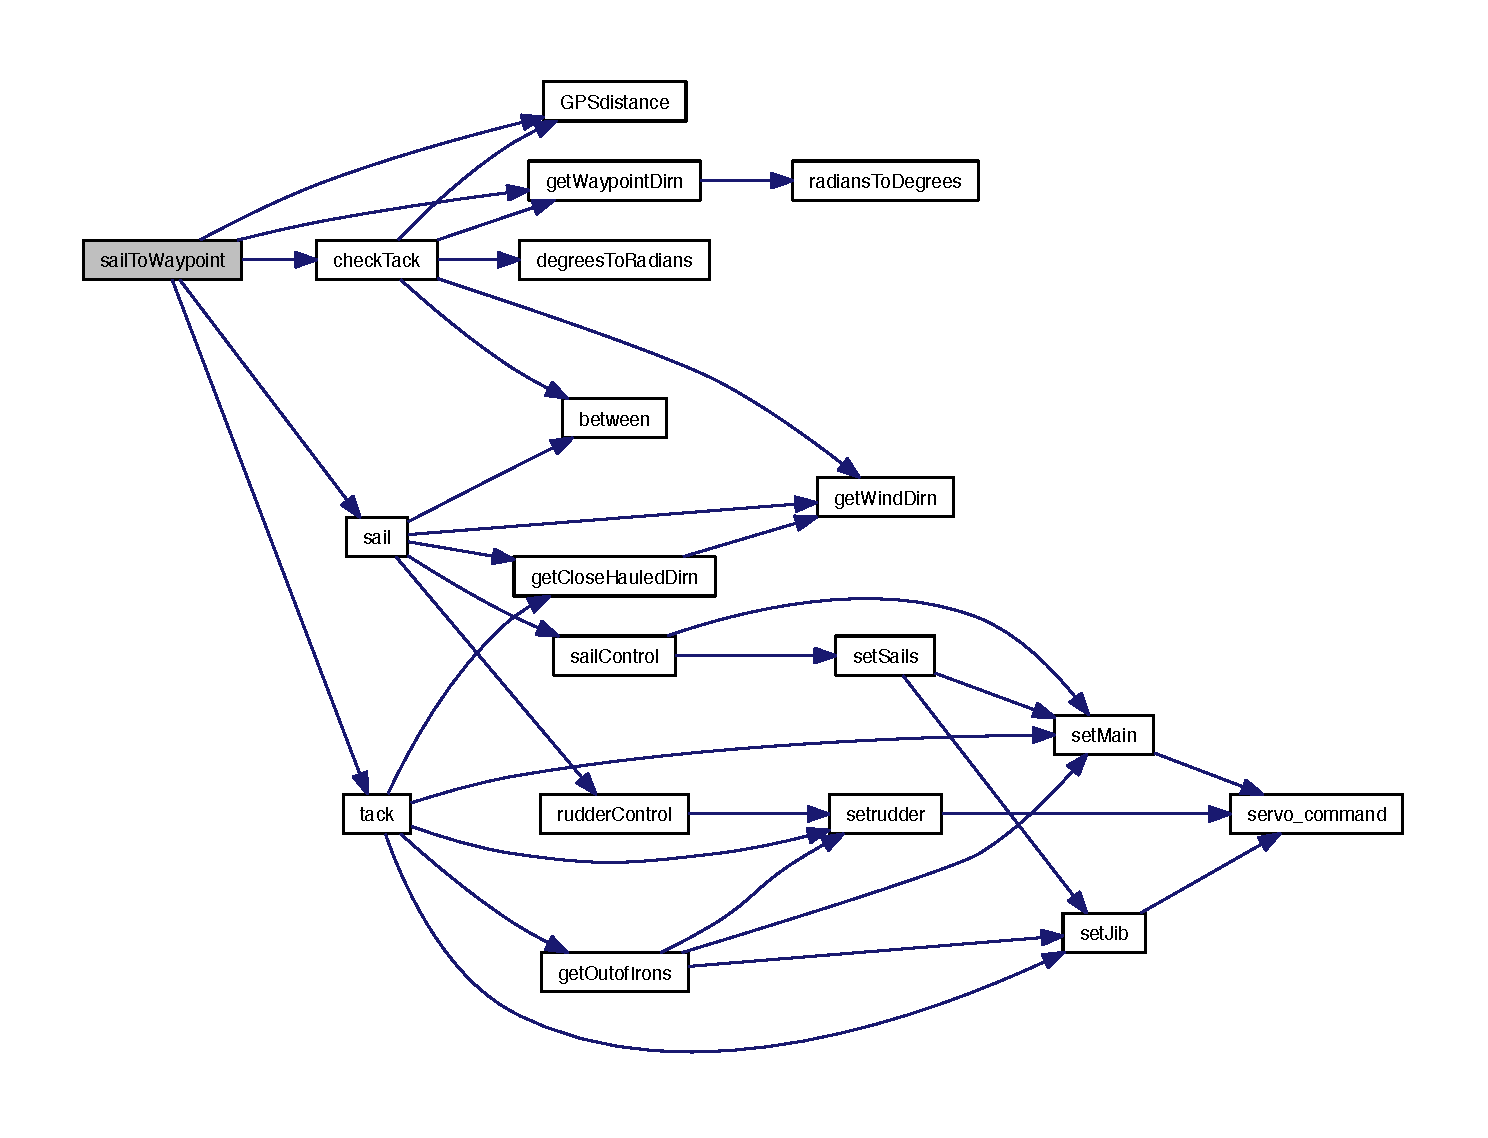
\includegraphics[width=350pt]{_sailing_logic_8pde_a42829044eaaf781783f525dbf35eabc1_cgraph}
\end{center}
\end{figure}




\-Here is the caller graph for this function\-:\nopagebreak
\begin{figure}[H]
\begin{center}
\leavevmode
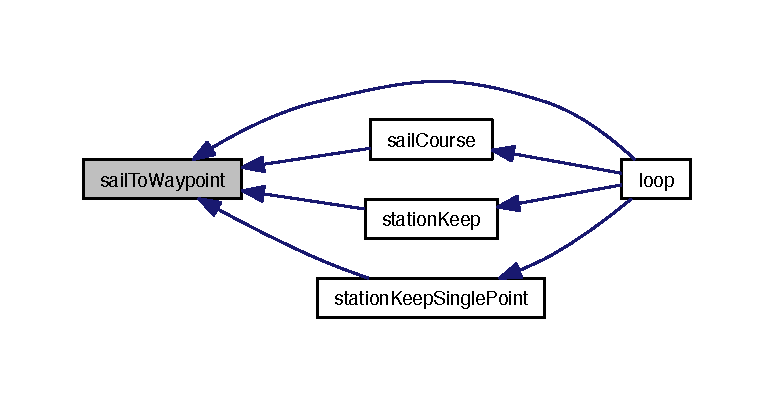
\includegraphics[width=350pt]{_sailing_logic_8pde_a42829044eaaf781783f525dbf35eabc1_icgraph}
\end{center}
\end{figure}



\hypertarget{_station_keeping_8pde}{
\section{/\-Users/allgood38/\-Desktop/qmast/sailcode\-\_\-alpha6/\-Station\-Keeping.pde \-File \-Reference}
\label{_station_keeping_8pde}\index{/\-Users/allgood38/\-Desktop/qmast/sailcode\-\_\-alpha6/\-Station\-Keeping.\-pde@{/\-Users/allgood38/\-Desktop/qmast/sailcode\-\_\-alpha6/\-Station\-Keeping.\-pde}}
}
\subsection*{\-Functions}
\begin{DoxyCompactItemize}
\item 
void \hyperlink{_station_keeping_8pde_a8781730c6d0b63baad8958328d7721e1}{get\-Station\-Keeping\-Centre} (double $\ast$centre\-Lat\-Min, double $\ast$centre\-Lon\-Min)
\item 
void \hyperlink{_station_keeping_8pde_a659621408d0c86bc3a5bc1d80214eaec}{fill\-Station\-Keeping\-Waypoints} (double centre\-Lat\-Min, double centre\-Lon\-Min, int wind\-Bearing)
\item 
int \hyperlink{_station_keeping_8pde_aa299757ffc71d051d673a238a5a4b387}{station\-Keep} ()
\item 
void \hyperlink{_station_keeping_8pde_a8582ebc297542fd91bbbdcb46b34cd24}{station\-Keep\-Single\-Point} ()
\end{DoxyCompactItemize}


\subsection{\-Function \-Documentation}
\hypertarget{_station_keeping_8pde_a659621408d0c86bc3a5bc1d80214eaec}{
\index{\-Station\-Keeping.\-pde@{\-Station\-Keeping.\-pde}!fill\-Station\-Keeping\-Waypoints@{fill\-Station\-Keeping\-Waypoints}}
\index{fill\-Station\-Keeping\-Waypoints@{fill\-Station\-Keeping\-Waypoints}!StationKeeping.pde@{\-Station\-Keeping.\-pde}}
\subsubsection[{fill\-Station\-Keeping\-Waypoints}]{\setlength{\rightskip}{0pt plus 5cm}void fill\-Station\-Keeping\-Waypoints (
\begin{DoxyParamCaption}
\item[{double}]{centre\-Lat\-Min, }
\item[{double}]{centre\-Lon\-Min, }
\item[{int}]{wind\-Bearing}
\end{DoxyParamCaption}
)}}
\label{_station_keeping_8pde_a659621408d0c86bc3a5bc1d80214eaec}


\-Definition at line 22 of file \-Station\-Keeping.\-pde.



\-Here is the caller graph for this function\-:\nopagebreak
\begin{figure}[H]
\begin{center}
\leavevmode
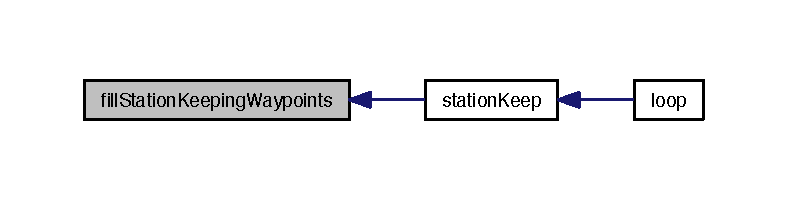
\includegraphics[width=350pt]{_station_keeping_8pde_a659621408d0c86bc3a5bc1d80214eaec_icgraph}
\end{center}
\end{figure}


\hypertarget{_station_keeping_8pde_a8781730c6d0b63baad8958328d7721e1}{
\index{\-Station\-Keeping.\-pde@{\-Station\-Keeping.\-pde}!get\-Station\-Keeping\-Centre@{get\-Station\-Keeping\-Centre}}
\index{get\-Station\-Keeping\-Centre@{get\-Station\-Keeping\-Centre}!StationKeeping.pde@{\-Station\-Keeping.\-pde}}
\subsubsection[{get\-Station\-Keeping\-Centre}]{\setlength{\rightskip}{0pt plus 5cm}void get\-Station\-Keeping\-Centre (
\begin{DoxyParamCaption}
\item[{double $\ast$}]{centre\-Lat\-Min, }
\item[{double $\ast$}]{centre\-Lon\-Min}
\end{DoxyParamCaption}
)}}
\label{_station_keeping_8pde_a8781730c6d0b63baad8958328d7721e1}


\-Definition at line 2 of file \-Station\-Keeping.\-pde.



\-Here is the caller graph for this function\-:\nopagebreak
\begin{figure}[H]
\begin{center}
\leavevmode
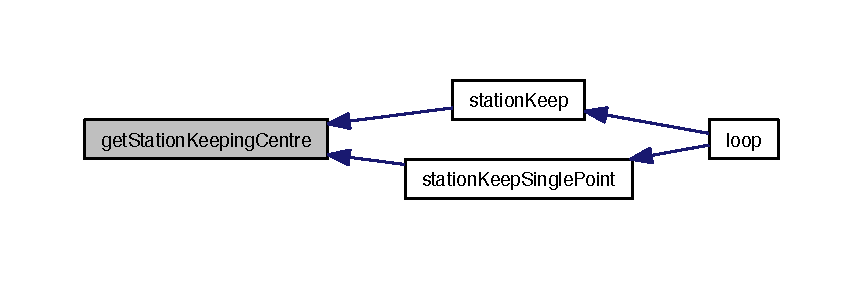
\includegraphics[width=350pt]{_station_keeping_8pde_a8781730c6d0b63baad8958328d7721e1_icgraph}
\end{center}
\end{figure}


\hypertarget{_station_keeping_8pde_aa299757ffc71d051d673a238a5a4b387}{
\index{\-Station\-Keeping.\-pde@{\-Station\-Keeping.\-pde}!station\-Keep@{station\-Keep}}
\index{station\-Keep@{station\-Keep}!StationKeeping.pde@{\-Station\-Keeping.\-pde}}
\subsubsection[{station\-Keep}]{\setlength{\rightskip}{0pt plus 5cm}int station\-Keep (
\begin{DoxyParamCaption}
{}
\end{DoxyParamCaption}
)}}
\label{_station_keeping_8pde_aa299757ffc71d051d673a238a5a4b387}


\-Definition at line 43 of file \-Station\-Keeping.\-pde.



\-Here is the call graph for this function\-:\nopagebreak
\begin{figure}[H]
\begin{center}
\leavevmode
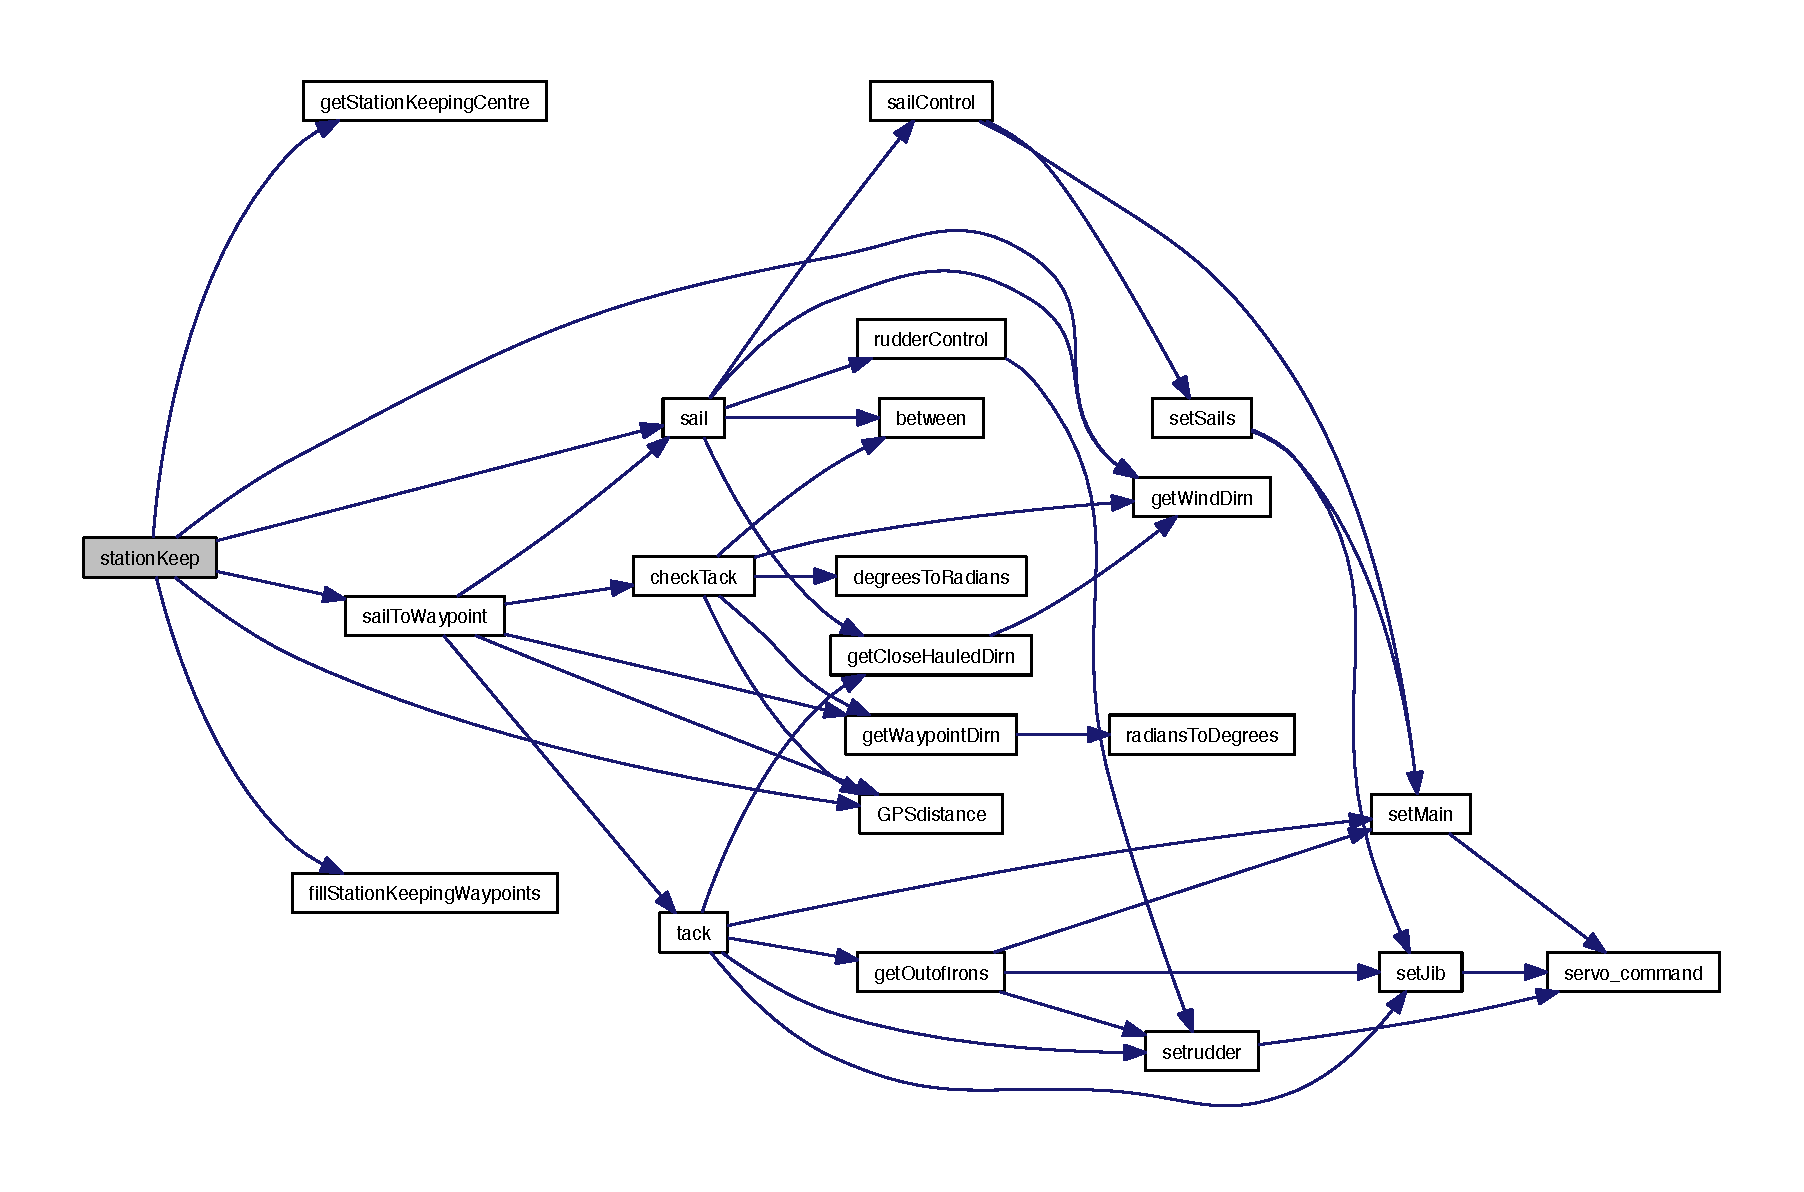
\includegraphics[width=350pt]{_station_keeping_8pde_aa299757ffc71d051d673a238a5a4b387_cgraph}
\end{center}
\end{figure}




\-Here is the caller graph for this function\-:\nopagebreak
\begin{figure}[H]
\begin{center}
\leavevmode
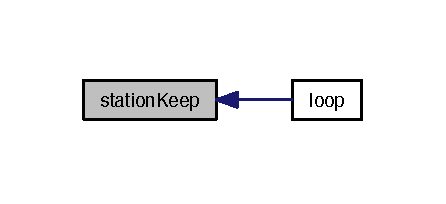
\includegraphics[width=214pt]{_station_keeping_8pde_aa299757ffc71d051d673a238a5a4b387_icgraph}
\end{center}
\end{figure}


\hypertarget{_station_keeping_8pde_a8582ebc297542fd91bbbdcb46b34cd24}{
\index{\-Station\-Keeping.\-pde@{\-Station\-Keeping.\-pde}!station\-Keep\-Single\-Point@{station\-Keep\-Single\-Point}}
\index{station\-Keep\-Single\-Point@{station\-Keep\-Single\-Point}!StationKeeping.pde@{\-Station\-Keeping.\-pde}}
\subsubsection[{station\-Keep\-Single\-Point}]{\setlength{\rightskip}{0pt plus 5cm}void station\-Keep\-Single\-Point (
\begin{DoxyParamCaption}
{}
\end{DoxyParamCaption}
)}}
\label{_station_keeping_8pde_a8582ebc297542fd91bbbdcb46b34cd24}


\-Definition at line 106 of file \-Station\-Keeping.\-pde.



\-Here is the call graph for this function\-:\nopagebreak
\begin{figure}[H]
\begin{center}
\leavevmode
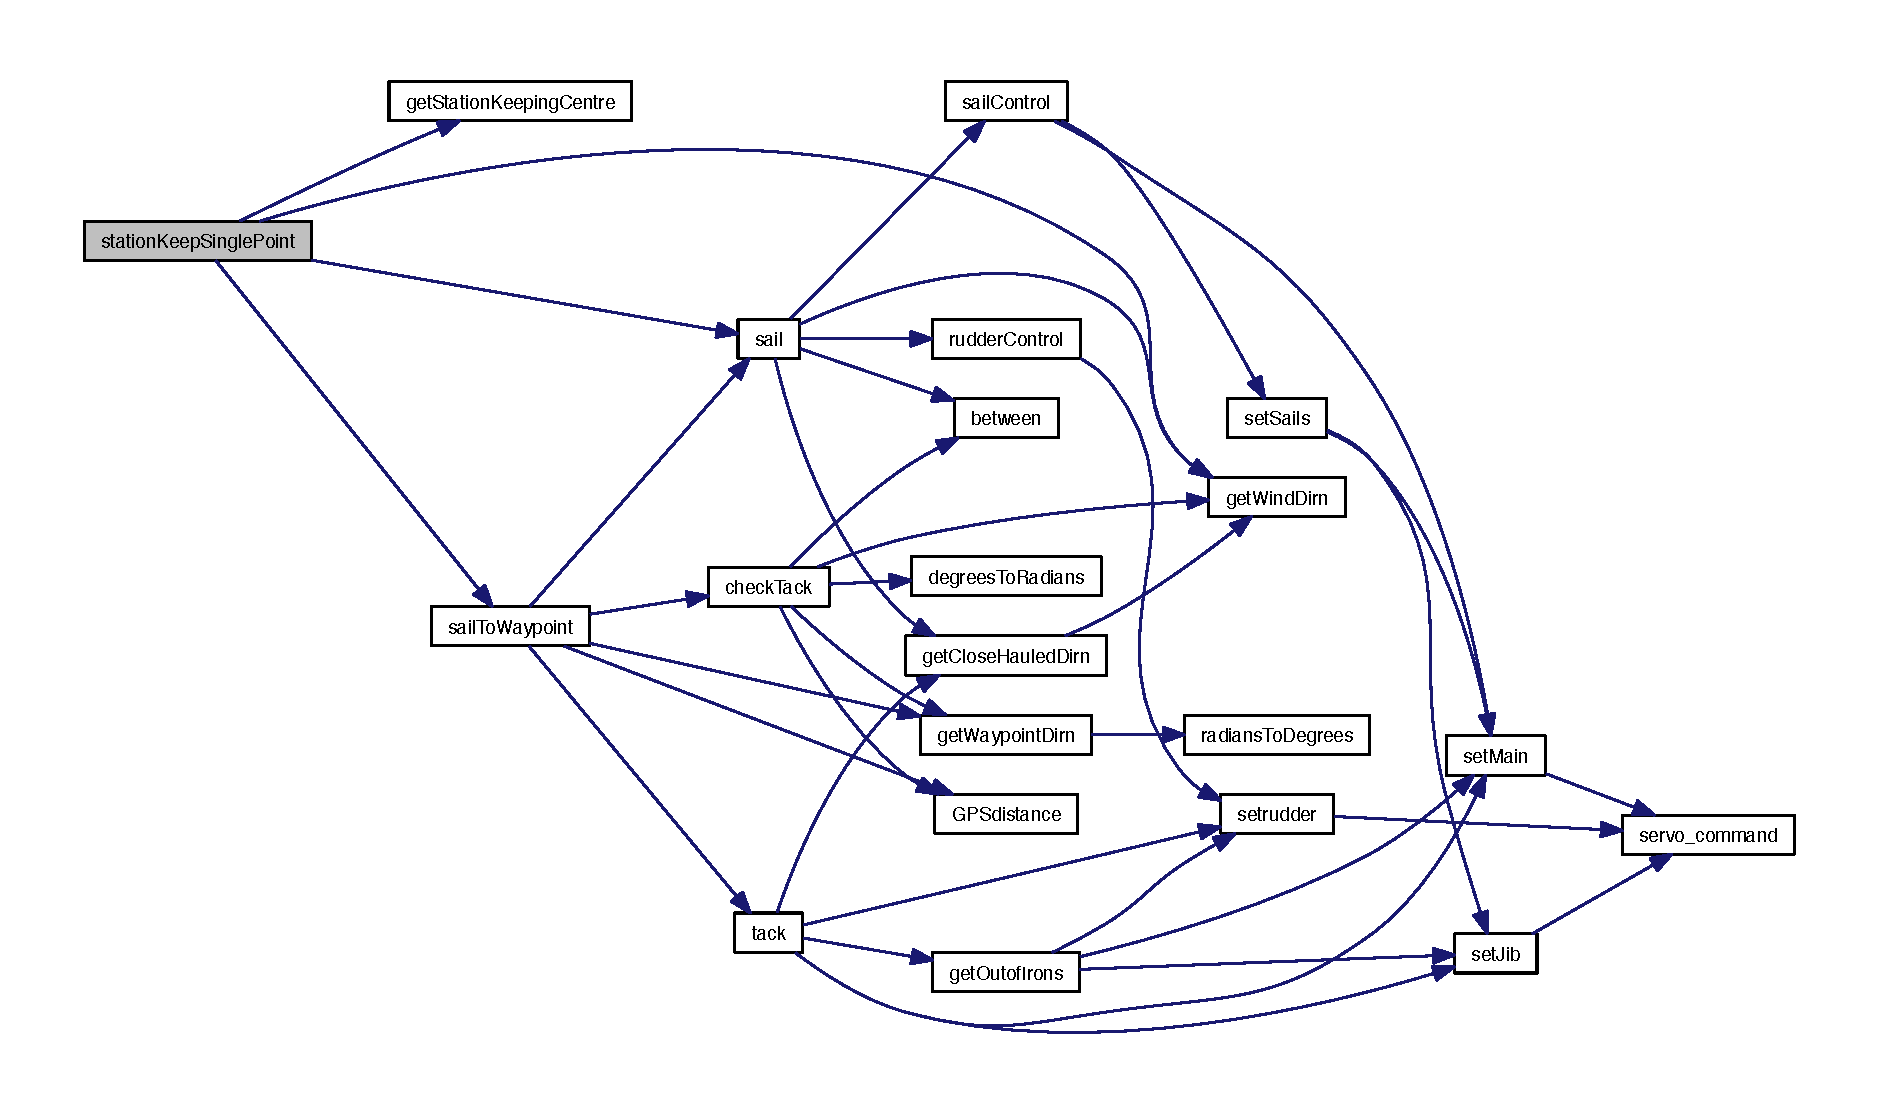
\includegraphics[width=350pt]{_station_keeping_8pde_a8582ebc297542fd91bbbdcb46b34cd24_cgraph}
\end{center}
\end{figure}




\-Here is the caller graph for this function\-:\nopagebreak
\begin{figure}[H]
\begin{center}
\leavevmode
\includegraphics[width=260pt]{_station_keeping_8pde_a8582ebc297542fd91bbbdcb46b34cd24_icgraph}
\end{center}
\end{figure}



\hypertarget{_tack_8pde}{
\section{/\-Users/allgood38/\-Desktop/qmast/sailcode\-\_\-alpha6/\-Tack.pde \-File \-Reference}
\label{_tack_8pde}\index{/\-Users/allgood38/\-Desktop/qmast/sailcode\-\_\-alpha6/\-Tack.\-pde@{/\-Users/allgood38/\-Desktop/qmast/sailcode\-\_\-alpha6/\-Tack.\-pde}}
}
\subsection*{\-Functions}
\begin{DoxyCompactItemize}
\item 
void \hyperlink{_tack_8pde_a6687f149db3a26da0af4bcb2c61fc9a3}{tack} ()
\item 
void \hyperlink{_tack_8pde_aa9b9ac04e546adfd9a330715867797de}{get\-Outof\-Irons} (int tackside)
\end{DoxyCompactItemize}


\subsection{\-Function \-Documentation}
\hypertarget{_tack_8pde_aa9b9ac04e546adfd9a330715867797de}{
\index{\-Tack.\-pde@{\-Tack.\-pde}!get\-Outof\-Irons@{get\-Outof\-Irons}}
\index{get\-Outof\-Irons@{get\-Outof\-Irons}!Tack.pde@{\-Tack.\-pde}}
\subsubsection[{get\-Outof\-Irons}]{\setlength{\rightskip}{0pt plus 5cm}void get\-Outof\-Irons (
\begin{DoxyParamCaption}
\item[{int}]{tackside}
\end{DoxyParamCaption}
)}}
\label{_tack_8pde_aa9b9ac04e546adfd9a330715867797de}


\-Definition at line 61 of file \-Tack.\-pde.



\-Here is the call graph for this function\-:\nopagebreak
\begin{figure}[H]
\begin{center}
\leavevmode
\includegraphics[width=350pt]{_tack_8pde_aa9b9ac04e546adfd9a330715867797de_cgraph}
\end{center}
\end{figure}




\-Here is the caller graph for this function\-:\nopagebreak
\begin{figure}[H]
\begin{center}
\leavevmode
\includegraphics[width=350pt]{_tack_8pde_aa9b9ac04e546adfd9a330715867797de_icgraph}
\end{center}
\end{figure}


\hypertarget{_tack_8pde_a6687f149db3a26da0af4bcb2c61fc9a3}{
\index{\-Tack.\-pde@{\-Tack.\-pde}!tack@{tack}}
\index{tack@{tack}!Tack.pde@{\-Tack.\-pde}}
\subsubsection[{tack}]{\setlength{\rightskip}{0pt plus 5cm}void tack (
\begin{DoxyParamCaption}
{}
\end{DoxyParamCaption}
)}}
\label{_tack_8pde_a6687f149db3a26da0af4bcb2c61fc9a3}


\-Definition at line 7 of file \-Tack.\-pde.



\-Here is the call graph for this function\-:\nopagebreak
\begin{figure}[H]
\begin{center}
\leavevmode
\includegraphics[width=350pt]{_tack_8pde_a6687f149db3a26da0af4bcb2c61fc9a3_cgraph}
\end{center}
\end{figure}




\-Here is the caller graph for this function\-:\nopagebreak
\begin{figure}[H]
\begin{center}
\leavevmode
\includegraphics[width=350pt]{_tack_8pde_a6687f149db3a26da0af4bcb2c61fc9a3_icgraph}
\end{center}
\end{figure}



\hypertarget{_testing___functions_8pde}{
\section{/\-Users/allgood38/\-Desktop/qmast/sailcode\-\_\-alpha6/\-Testing\-\_\-\-Functions.pde \-File \-Reference}
\label{_testing___functions_8pde}\index{/\-Users/allgood38/\-Desktop/qmast/sailcode\-\_\-alpha6/\-Testing\-\_\-\-Functions.\-pde@{/\-Users/allgood38/\-Desktop/qmast/sailcode\-\_\-alpha6/\-Testing\-\_\-\-Functions.\-pde}}
}

\hypertarget{_transmit_8pde}{
\section{/\-Users/allgood38/\-Desktop/qmast/sailcode\-\_\-alpha6/\-Transmit.pde \-File \-Reference}
\label{_transmit_8pde}\index{/\-Users/allgood38/\-Desktop/qmast/sailcode\-\_\-alpha6/\-Transmit.\-pde@{/\-Users/allgood38/\-Desktop/qmast/sailcode\-\_\-alpha6/\-Transmit.\-pde}}
}
\subsection*{\-Functions}
\begin{DoxyCompactItemize}
\item 
void \hyperlink{_transmit_8pde_a29ff55f7ca3b7d4a69af0648518423a3}{transmit} (void)
\begin{DoxyCompactList}\small\item\em \-The transmit function is used to communicate with \-Lab\-View. \end{DoxyCompactList}\item 
void \hyperlink{_transmit_8pde_a8b1a977963d6dc483e5ca8bd2ffde8c9}{relay\-Data} ()
\begin{DoxyCompactList}\small\item\em \-Similar to the transmit function except the output contains information which is not read by \-Lab\-View, so codes are not needed? \end{DoxyCompactList}\end{DoxyCompactItemize}


\subsection{\-Function \-Documentation}
\hypertarget{_transmit_8pde_a8b1a977963d6dc483e5ca8bd2ffde8c9}{
\index{\-Transmit.\-pde@{\-Transmit.\-pde}!relay\-Data@{relay\-Data}}
\index{relay\-Data@{relay\-Data}!Transmit.pde@{\-Transmit.\-pde}}
\subsubsection[{relay\-Data}]{\setlength{\rightskip}{0pt plus 5cm}void relay\-Data (
\begin{DoxyParamCaption}
{}
\end{DoxyParamCaption}
)}}
\label{_transmit_8pde_a8b1a977963d6dc483e5ca8bd2ffde8c9}


\-Similar to the transmit function except the output contains information which is not read by \-Lab\-View, so codes are not needed? 

\-Latitude and longitude of boat's location, split into more precise degrees and minutes, to fit into a float 

\-Definition at line 60 of file \-Transmit.\-pde.

\hypertarget{_transmit_8pde_a29ff55f7ca3b7d4a69af0648518423a3}{
\index{\-Transmit.\-pde@{\-Transmit.\-pde}!transmit@{transmit}}
\index{transmit@{transmit}!Transmit.pde@{\-Transmit.\-pde}}
\subsubsection[{transmit}]{\setlength{\rightskip}{0pt plus 5cm}void transmit (
\begin{DoxyParamCaption}
\item[{void}]{}
\end{DoxyParamCaption}
)}}
\label{_transmit_8pde_a29ff55f7ca3b7d4a69af0648518423a3}


\-The transmit function is used to communicate with \-Lab\-View. 

through a series of preset strings, which are represented by the graphical gauges?

\-Prints directly to the serial and takes input from global values 

\-Definition at line 8 of file \-Transmit.\-pde.



\-Here is the caller graph for this function\-:\nopagebreak
\begin{figure}[H]
\begin{center}
\leavevmode
\includegraphics[width=302pt]{_transmit_8pde_a29ff55f7ca3b7d4a69af0648518423a3_icgraph}
\end{center}
\end{figure}



\hypertarget{_utilities_8pde}{
\section{/\-Users/allgood38/\-Desktop/qmast/sailcode\-\_\-alpha6/\-Utilities.pde \-File \-Reference}
\label{_utilities_8pde}\index{/\-Users/allgood38/\-Desktop/qmast/sailcode\-\_\-alpha6/\-Utilities.\-pde@{/\-Users/allgood38/\-Desktop/qmast/sailcode\-\_\-alpha6/\-Utilities.\-pde}}
}
\subsection*{\-Functions}
\begin{DoxyCompactItemize}
\item 
float \hyperlink{_utilities_8pde_afe25c7411bef33d33beaa8f6bf6e07e7}{degrees\-To\-Radians} (int angle)
\item 
int \hyperlink{_utilities_8pde_abcc11dba11f0d39f4ab19c05f1d5fe75}{radians\-To\-Degrees} (float angle)
\item 
boolean \hyperlink{_utilities_8pde_acf7fddcdef68f94ad48b357770aebac5}{between} (int angle, int a, int b)
\item 
char \hyperlink{_utilities_8pde_acdb581c51e99361f7c3f648a9ee7e862}{convert\-A\-S\-C\-I\-Ito\-Hex} (const char ch)
\end{DoxyCompactItemize}


\subsection{\-Function \-Documentation}
\hypertarget{_utilities_8pde_acf7fddcdef68f94ad48b357770aebac5}{
\index{\-Utilities.\-pde@{\-Utilities.\-pde}!between@{between}}
\index{between@{between}!Utilities.pde@{\-Utilities.\-pde}}
\subsubsection[{between}]{\setlength{\rightskip}{0pt plus 5cm}boolean between (
\begin{DoxyParamCaption}
\item[{int}]{angle, }
\item[{int}]{a, }
\item[{int}]{b}
\end{DoxyParamCaption}
)}}
\label{_utilities_8pde_acf7fddcdef68f94ad48b357770aebac5}


\-Definition at line 12 of file \-Utilities.\-pde.



\-Here is the caller graph for this function\-:\nopagebreak
\begin{figure}[H]
\begin{center}
\leavevmode
\includegraphics[width=350pt]{_utilities_8pde_acf7fddcdef68f94ad48b357770aebac5_icgraph}
\end{center}
\end{figure}


\hypertarget{_utilities_8pde_acdb581c51e99361f7c3f648a9ee7e862}{
\index{\-Utilities.\-pde@{\-Utilities.\-pde}!convert\-A\-S\-C\-I\-Ito\-Hex@{convert\-A\-S\-C\-I\-Ito\-Hex}}
\index{convert\-A\-S\-C\-I\-Ito\-Hex@{convert\-A\-S\-C\-I\-Ito\-Hex}!Utilities.pde@{\-Utilities.\-pde}}
\subsubsection[{convert\-A\-S\-C\-I\-Ito\-Hex}]{\setlength{\rightskip}{0pt plus 5cm}char convert\-A\-S\-C\-I\-Ito\-Hex (
\begin{DoxyParamCaption}
\item[{const char}]{ch}
\end{DoxyParamCaption}
)}}
\label{_utilities_8pde_acdb581c51e99361f7c3f648a9ee7e862}


\-Definition at line 49 of file \-Utilities.\-pde.



\-Here is the caller graph for this function\-:\nopagebreak
\begin{figure}[H]
\begin{center}
\leavevmode
\includegraphics[width=350pt]{_utilities_8pde_acdb581c51e99361f7c3f648a9ee7e862_icgraph}
\end{center}
\end{figure}


\hypertarget{_utilities_8pde_afe25c7411bef33d33beaa8f6bf6e07e7}{
\index{\-Utilities.\-pde@{\-Utilities.\-pde}!degrees\-To\-Radians@{degrees\-To\-Radians}}
\index{degrees\-To\-Radians@{degrees\-To\-Radians}!Utilities.pde@{\-Utilities.\-pde}}
\subsubsection[{degrees\-To\-Radians}]{\setlength{\rightskip}{0pt plus 5cm}float degrees\-To\-Radians (
\begin{DoxyParamCaption}
\item[{int}]{angle}
\end{DoxyParamCaption}
)}}
\label{_utilities_8pde_afe25c7411bef33d33beaa8f6bf6e07e7}


\-Definition at line 3 of file \-Utilities.\-pde.



\-Here is the caller graph for this function\-:\nopagebreak
\begin{figure}[H]
\begin{center}
\leavevmode
\includegraphics[width=350pt]{_utilities_8pde_afe25c7411bef33d33beaa8f6bf6e07e7_icgraph}
\end{center}
\end{figure}


\hypertarget{_utilities_8pde_abcc11dba11f0d39f4ab19c05f1d5fe75}{
\index{\-Utilities.\-pde@{\-Utilities.\-pde}!radians\-To\-Degrees@{radians\-To\-Degrees}}
\index{radians\-To\-Degrees@{radians\-To\-Degrees}!Utilities.pde@{\-Utilities.\-pde}}
\subsubsection[{radians\-To\-Degrees}]{\setlength{\rightskip}{0pt plus 5cm}int radians\-To\-Degrees (
\begin{DoxyParamCaption}
\item[{float}]{angle}
\end{DoxyParamCaption}
)}}
\label{_utilities_8pde_abcc11dba11f0d39f4ab19c05f1d5fe75}


\-Definition at line 8 of file \-Utilities.\-pde.



\-Here is the caller graph for this function\-:\nopagebreak
\begin{figure}[H]
\begin{center}
\leavevmode
\includegraphics[width=350pt]{_utilities_8pde_abcc11dba11f0d39f4ab19c05f1d5fe75_icgraph}
\end{center}
\end{figure}



\printindex
\end{document}
